%======================================================================================================================
% SLO: definiraj strukturo dokumenta
% ENG: define file structure
%======================================================================================================================
\documentclass[a4paper, 12pt]{book}
\usepackage[T1]{fontenc}
% to doda lomljenje besed v več vrstic, a je to v redu?
\usepackage[htt]{hyphenat}

%======================================================================================================================
% SLO: Odkomentiraj "\SLOtrue " za izbiro slovenskega jezika
% ENG: Uncomment "\SLOfalse" to chose English language
%======================================================================================================================
\newif\ifSLO
\newif\ifTRACKEXIST
\newif\ifTRACKCS
\newif\ifPROGRAMMM

% ---------------------------------------------------------------------------------------------------------------------
% IMPORTANT: Adjust the thesis language, your study program and course within this block
%  --------------------------------------------------------------------------------------------------------------------
% switch language
\SLOtrue % Enables Slovenian language
%\SLOfalse  % Enables English language

% switch programs: Computer science and Multimedia. Set to false if the program is in Multimedia
\PROGRAMMMfalse
%\PROGRAMMMtrue

% switch on if your program is divided into tracks CS and DS, otherwise leave it false
% CAUTION: if you were first enrolled into your program before school year 2019/2020, your program is not divided
% into tracks. In any case, be absolutely sure you select the correct variant. IF IN DOUBT, always contact the
% student office to advise you.
%
\TRACKEXISTfalse
%\TRACKEXISTtrue

% default course name is "Computer science" if your course name is "Data science", set the following switch to false
\TRACKCStrue % uncomment if the thesis is from course "Information science"
%\TRACKCSfalse % uncomment if the thesis is from course "Data Science"
% ---------------------------------------------------------------------------------------------------------------------
% End of language, program and course adjustment
% ---------------------------------------------------------------------------------------------------------------------


%======================================================================================================================
% SLO: vključi oblikovanje in pakete
% ENG: include design and packages
%======================================================================================================================
%----------------------------------------------------------------
% SLO: LaTeX paketi
% ENG: LateX packages
%----------------------------------------------------------------
% SLO: omogoča uporabo slovenskih (latinskih) črk kodiranih v formatu UTF-8
% ENG: enables the use of slovene (latin) caracters encoded in the UFT-8 format
\usepackage[utf8]{inputenc}
%\inputencoding{utf8}
% SLO: naloži, med drugim, slovenske delilne vzorce
% ENG: loads, among others, slovene dividing patterns
\usepackage[slovene,english]{babel}
% SLO: poskrbi za postavitev strani
% ENG: takes care of the page layout
\usepackage{fancyhdr}
% SLO: za vlaganje slik različnih formatov
% ENG: for loading figures of different formats
\usepackage{graphicx}
\usepackage{caption}
\captionsetup[figure]{labelfont=bf} % SLO: napis "Slika #" v krepkem tisku
									% ENG: wirte "Figure #" caption in bold
\captionsetup[table]{labelfont=bf} % SLO: napis "Tabela #" v krepkem tisku
								   % ENG: wirte "Table #" caption in bold
% SLO: za pisanje psevdokode
% ENG: for writing pseudocode
\usepackage{algorithm}
\usepackage{algorithmic}
\floatname{algorithm}{\footnotesize Algorithm} % SLO: napis "Algoritem #" v krepkem tisku
											   % ENG: write "Algorithm #" caption in bold
% SLO: poveže reference slik/tabel in slike/tabele znotraj dokumenta
% ENG: links image/table references with the images/tables within the document
\usepackage[pdfa]{hyperref}
% SLO: pri kliku na referenco slike/tabele se postavi na vrh slike/tabele
% ENG: when clicking the image/table reference, position the focus on top of the image/table
\usepackage[all]{hypcap}
% SLO: omogoča, med drugim, definicjo in uporebo barve
% ENG: enables, among others, the definition and use of colors
\usepackage{xcolor}
%----------------------------------------------------------------
% SLO: dodatni paketi
% ENG: additional packages
%----------------------------------------------------------------
% SLO: omogoča večjo manipulacijo nad tabelami
% ENG: allows for greater manipulation of tables
\usepackage{booktabs}
% SLO: naloži dodatne simbole
% ENG: loads additional symbols
\usepackage{amssymb}
% SLO: omogoča, med drugim, sklicevanje na formule z eqref
% ENG: enables, among others, equation referencing with eqref
\usepackage{amsmath}
% SLO: omogoča komentiranje večjega dela teksta
% ENG: enables the commenting of larger text parts
\usepackage{verbatim}
% SLO: omogoča rotacijo PDF strani v ležeč položaj
% ENG: enables the rotation of a PDF page to landscape
\usepackage{pdflscape}
% SLO: omogoča barvanje vrstic in stolpcev tabel
% ENG: enables coloring of table rows and columns
\usepackage{colortbl}
\usepackage{url}
\usepackage{tabularx}



%================================================================
% SLO: nastavitve dokumenta
% ENG: document properties
%================================================================
% SLO: prilagoditev robov za tisk
% ENG: margin adjustments for printing
\addtolength{\marginparwidth}{-20pt}
\addtolength{\oddsidemargin}{40pt}
\addtolength{\evensidemargin}{-40pt}
% SLO: razmik med vrsticami
% ENG: line spacing
\renewcommand{\baselinestretch}{1.3}
% SLO: postavitev strani
% ENG: page layout
\renewcommand{\chaptermark}[1]{\markboth{\MakeUppercase{\thechapter.\ #1}}{}}
\renewcommand{\sectionmark}[1]{\markright{\MakeUppercase{\thesection.\ #1}}}
\renewcommand{\headrulewidth}{0.5pt} % Header rule
\renewcommand{\footrulewidth}{0pt} % Footer rule
%
\fancypagestyle{frontmatter}{%
	\fancyhf{} % Clear all headers and footers first
	\fancyhead[LE, RO]{\sl \thepage}
	%\fancyhead[LO]{\sl \rightmark}
	%\fancyhead[RE]{\sl \leftmark}
}
\fancypagestyle{mainmatter}{%
  	\fancyhf{} % Clear all headers and footers first
	\fancyhead[LE,RO]{\sl \thepage}
	\fancyhead[LO]{\sl \rightmark}
	\fancyhead[RE]{\sl \leftmark}
}
% SLO: font za ime avtorja
% ENG: font for author name
\newcommand{\authorfont}{\Large}
% SLO: font za naslov diplomskega dela
% ENG: font for thesis title
\newcommand{\titlefont}{\LARGE\bf}
% SLO: globina kazala
% ENG: content depth
\setcounter{tocdepth}{1}
% SLO: definiraj ukaz za prazno stran
% ENG: define the command for empty page
\newcommand{\clearemptydoublepage}{\newpage{\pagestyle{empty}\cleardoublepage}}

% course title
\newcommand{\trackname}{!undefined!}

\newcommand{\BibTeX}{{\sc Bib}\TeX}




%----------------------------------------------------------------------------------------------------------------------
% |||||||||||||||||||||| USTREZNO POPRAVI |||||||||||||||||||||||
% |||||||||||||||||||||| EDIT ACCORDINGLY |||||||||||||||||||||||
%----------------------------------------------------------------------------------------------------------------------
\newcommand{\ttitle}{Neprekinjena integracija in dostava poslovno kritičnih aplikacij}
\newcommand{\ttitleEn}{Continuous integration and delivery for business critical applications}
\newcommand{\tsubject}{\ttitle}
\newcommand{\tsubjectEn}{\ttitleEn}
\newcommand{\tauthor}{Jakob Maležič}
\newcommand{\temail}{jm6421@student.uni-lj.si}
\newcommand{\myyear}{2023}
\newcommand{\tkeywords}{neprekinjena integracija, neprekinjena dostava, poslovno kritične aplikacije, platforma GitLab}
\newcommand{\tkeywordsEn}{continuous integration, continuous deployment, business critical applications, GitLab platform}
\newcommand{\mysupervisor}{doc.~dr.\ Nejc Ilc}
\newcommand{\mycosupervisor}{dr.\ Tadej Justin}

% include formatted front pages

%----------------------------------------------------------------
% SLO: definiraj metapodatke za datoteko master_thesis.tex
% ENG: define metadata for the file master_thesis.tex
%----------------------------------------------------------------
%----------------------------------------------------------------
%	HYPERREF SETUP
% SLO: ustrezno popravi e-mail
% ENG: edit the e-mail accordingly
%----------------------------------------------------------------
\hypersetup{pdftitle={\ttitle}}
\hypersetup{pdfsubject=\ttitleEn}
\hypersetup{pdfauthor={\tauthor, \temail}}
\hypersetup{pdfkeywords=\tkeywordsEn}

%----------------------------------------------------------------
% define medatata
% SLO: ustrezno popravi e-mail
% ENG: edit the e-mail accordingly
%----------------------------------------------------------------
\def\Title{\ttitle}
\def\Author{\tauthor, \temail}
\def\Subject{\ttitleEn}
\def\Keywords{\tkeywordsEn}
\def\Org{Univerza v Ljubljani, Fakulteta za računalništvo in informatiko}

%%%%%%%%%%%%%%%%%%%%%%%%%%%%%%%%%%%%%%%%
% \convertDate converts D:20080419103507+02'00' to 2008-04-19T10:35:07+02:00
%%%%%%%%%%%%%%%%%%%%%%%%%%%%%%%%%%%%%%%%
\def\convertDate{%
    \getYear
}

{\catcode`\D=12
 \gdef\getYear D:#1#2#3#4{\edef\xYear{#1#2#3#4}\getMonth}
}
\def\getMonth#1#2{\edef\xMonth{#1#2}\getDay}
\def\getDay#1#2{\edef\xDay{#1#2}\getHour}
\def\getHour#1#2{\edef\xHour{#1#2}\getMin}
\def\getMin#1#2{\edef\xMin{#1#2}\getSec}
\def\getSec#1#2{\edef\xSec{#1#2}\getTZh}
\def\getTZh +#1#2{\edef\xTZh{#1#2}\getTZm}
\def\getTZm '#1#2'{%
    \edef\xTZm{#1#2}%
    \edef\convDate{\xYear-\xMonth-\xDay T\xHour:\xMin:\xSec+\xTZh:\xTZm}%
}

\expandafter\convertDate\pdfcreationdate


%%%%%%%%%%%%%%%%%%%%%%%%%%%%%%%%%%%%%%%%
% get pdftex version string
%%%%%%%%%%%%%%%%%%%%%%%%%%%%%%%%%%%%%%%%
\newcount\countA
\countA=\pdftexversion
\advance \countA by -100
\def\pdftexVersionStr{pdfTeX-1.\the\countA.\pdftexrevision}

%%%%%%%%%%%%%%%%%%%%%%%%%%%%%%%%%%%%%%%%
% XMP data
%%%%%%%%%%%%%%%%%%%%%%%%%%%%%%%%%%%%%%%%
\usepackage{xmpincl}
\includexmp{pdfa-1b}

%%%%%%%%%%%%%%%%%%%%%%%%%%%%%%%%%%%%%%%%
% pdfInfo
%%%%%%%%%%%%%%%%%%%%%%%%%%%%%%%%%%%%%%%%
\pdfinfo{%
    /Title    (\ttitle)
    /Author   (\tauthor, \temail)
    /Subject  (\ttitleEn)
    /Keywords (\tkeywordsEn)
    /ModDate  (\pdfcreationdate)
    /Trapped  /False
}

%================================================================
% SLO: razno
% ENG: other
%================================================================
% SLO: nastavitev sklicevanj
% ENG: hyper referencing setup
\definecolor{black}{rgb}{0,0,0}
\hypersetup{
	colorlinks = true,
	linkcolor = black,
	citecolor = black,
	urlcolor = black
}

%----------------------------------------------------------------
% SLO: dodaj poti do datotek s slikami
% ENG: add paths to files containing figures
%----------------------------------------------------------------
\graphicspath{
	{figures/}
	{tables/}
}
%----------------------------------------------------------------
% SLO: moji paketi
% ENG: my packages
%----------------------------------------------------------------
% ...
%----------------------------------------------------------------
% SLO: moji konstrukti
% ENG: my constructs
%----------------------------------------------------------------
\newtheorem{izrek}{Izrek}[chapter]
\newtheorem{trditev}{Trditev}[izrek]
\newenvironment{dokaz}{\emph{Dokaz.}\ }{\hspace{\fill}{$\Box$}}

\newcommand{\CcImageCc}[1]{%
	\includegraphics[scale=#1]{cc-licenca/cc_cc_30.pdf}%
}
\newcommand{\CcImageBy}[1]{%
	\includegraphics[scale=#1]{cc-licenca/cc_by_30.pdf}%
}
\newcommand{\CcImageSa}[1]{%
	\includegraphics[scale=#1]{cc-licenca/cc_sa_30.pdf}%
}

%================================================================
% SLO: začetne strani magistrskega dela
% ENG: fist pages of the master's thesis
%================================================================
\begin{document}
% SLO: prepreči težave s številkami strani v kazalu
% ENG: prevents problems with the page numbers in the contents page
\renewcommand{\thepage}{}

%----------------------------------------------------------------
% Language-dependent formatting
%----------------------------------------------------------------
\ifSLO
    % SLO: definiraj slovensko besedo za kazalo
    \renewcommand{\contentsname}{Kazalo}

    % SLO: naslovnica
    % select the course title if it exist
\ifTRACKEXIST
    \ifTRACKCS
        \renewcommand{\trackname}{Računalništvo in Informatika}
    \else
        \renewcommand{\trackname}{Podatkovne Vede}
    \fi
\fi

\ifPROGRAMMM
    \thispagestyle{empty}
    \begin{center}
        {\large\sc Univerza v Ljubljani\\Fakulteta za računalništvo in informatiko\\
            Fakulteta za elektrotehniko}
    	   \vskip 10em
    	   {\authorfont \tauthor \par}
    	   {\titlefont \ttitle \par}
        {\vskip 2em \textsc{MAGISTRSKO DELO\\[2mm]
        MAGISTRSKI ŠTUDIJSKI PROGRAM DRUGE STOPNJE\\MULTIMEDIJA
        }\par}
        \vfill\null
        {\large \textsc{Mentor}: \mysupervisor \par}
   	    {\large \textsc{Somentor}: \mycosupervisor \par}
        {\vskip 2em \large Ljubljana, \myyear \par}
   \end{center}
\else
    \thispagestyle{empty}
	\begin{center}
            {\large\sc Univerza v Ljubljani\\Fakulteta za računalništvo in informatiko}
    	   \vskip 10em
    	   {\authorfont \tauthor \par}
    	   {\titlefont \ttitle \par}
        {\vskip 2em \textsc{MAGISTRSKO DELO\\[2mm]
        ŠTUDIJSKI PROGRAM DRUGE STOPNJE\\RAČUNALNIŠTVO IN INFORMATIKA
        \ifTRACKEXIST
            \\Smer: \trackname
        \fi
        }\par}
        \vfill\null
        {\large \textsc{Mentor}: \mysupervisor \par}
   	    {\large \textsc{Somentor}: \mycosupervisor \par}
        {\vskip 2em \large Ljubljana, \myyear \par}
   \end{center}
\fi  \clearemptydoublepage
    % SLO: avtorske pravice
    \thispagestyle{empty}
\vspace*{\fill}
{\noindent\footnotesize
{\sc Avtorske pravice}. 
\ifPROGRAMMM
    Rezultati magistrskega dela so intelektualna lastnina avtorja, Fakultete za ra\-ču\-nal\-niš\-tvo in informatiko ter Fakultete za Elektrotehniko Univerze v Ljubljani. Za objavljanje ali izkoriščanje rezultatov ma\-gi\-str\-ske\-ga dela je potrebno pisno soglasje avtorja, Fakultete za ra\-ču\-nal\-niš\-tvo in informatiko, Fakultete za Elektrotehniko ter mentorja\footnote{V dogovorju z mentorjem lahko kandidat magistrsko delo s pripadajočo izvorno kodo izda tudi pod drugo licenco, ki ponuja določen del pravic vsem: npr. Creative Commons, GNU GPL. V tem primeru na to mesto vstavite opis licence, na primer tekst~\cite{licence}.}.
\else
    Rezultati magistrskega dela so intelektualna lastnina avtorja in Fakultete za ra\-ču\-nal\-niš\-tvo in informatiko Univerze v Ljubljani. Za objavljanje ali izkoriščanje rezultatov ma\-gi\-str\-ske\-ga dela je potrebno pisno soglasje avtorja, Fakultete za ra\-ču\-nal\-niš\-tvo in informatiko ter mentorja\footnote{V dogovorju z mentorjem lahko kandidat magistrsko delo s pripadajočo izvorno kodo izda tudi pod drugo licenco, ki ponuja določen del pravic vsem: npr. Creative Commons, GNU GPL. V tem primeru na to mesto vstavite opis licence, na primer tekst~\cite{licence}.}.
\fi    
}
\begin{center}
{\footnotesize{\sc \copyright \myyear\ \tauthor}}
\end{center}  \clearemptydoublepage
    % SLO: izjava o avtorstvu (ni več del vezane izdaje, ločena oddaja)
    % SLO: zahvala
    \thispagestyle{empty}

\begin{center}
{\Large \textbf{\sc Zahvala}}
\end{center}
\vspace{0.5cm}

{\it\noindent
Rad bi se zahvalil svoji družini, še posebej svojim staršem, za vzpodbudo in podporo tekom mojega študija, zaročenki Maši za potrpežljivost in pomoč pri pisanju, mentorjema doc. dr. Nejcu Ilcu in dr. Tadeju Justinu za mentorstvo in nasvete, sodelavcu Roku Koleša za vso pomoč pri reševanju izzivov, in podjetju Medius, da mi je omogočilo pisanje magistrske naloge ter priskrbelo zanimivo temo.

\vspace{0.5cm} \hfill \tauthor, \myyear
} \clearemptydoublepage
    % SLO: posvetilo
    \thispagestyle{empty}\mbox{}{\vskip0.20\textheight}\mbox{}\hfill\begin{minipage}{0.55\textwidth}%

Vsem rožicam tega sveta.\\\\
\textit{''The only reason for time is so that everything doesn't happen at once.''}
\flushright --- Albert Einstein
\normalfont\end{minipage} \clearemptydoublepage
\else

    % ENG: title page ENG
    % select the course title if it exist
\ifTRACKEXIST
    \ifTRACKCS
        \renewcommand{\trackname}{Computer and Information Science}
    \else
        \renewcommand{\trackname}{Data Science}
    \fi
\fi

\ifPROGRAMMM
    \thispagestyle{empty}
	\begin{center}
        {\large\sc University of Ljubljana\\Faculty of Computer and Information Science\\
        Faculty of Electrical Engineering}
    	\vskip 10em
    	{\authorfont \tauthor \par}
    	{\titlefont \ttitleEn \par}
        {\vskip 2em \textsc{MASTER'S THESIS\\[2mm]
        THE 2nd CYCLE MASTER'S STUDY PROGRAMME\\MULTIMEDIA
        }\par}
        \vfill\null
        {\large \textsc{Supervisor}: \mysupervisor \par}
   	    {\large \textsc{Co-supervisor}:  \mycosupervisor \par}
        {\vskip 2em \large Ljubljana, \myyear \par}
   \end{center}
\else
    \thispagestyle{empty}
	\begin{center}
        {\large\sc University of Ljubljana\\Faculty of Computer and Information Science}
    	\vskip 10em
    	{\authorfont \tauthor \par}
    	{\titlefont \ttitleEn \par}
        {\vskip 2em \textsc{MASTER'S THESIS\\[2mm]
        THE 2nd CYCLE MASTER'S STUDY PROGRAMME\\COMPUTER AND INFORMATION SCIENCE
        \ifTRACKEXIST
            \\Track: \trackname
        \fi
        }\par}
        \vfill\null
        {\large \textsc{Supervisor}: \mysupervisor \par}
   	    {\large \textsc{Co-supervisor}:  \mycosupervisor \par}
        {\vskip 2em \large Ljubljana, \myyear \par}
    \end{center}
\fi  \clearemptydoublepage
    % ENG: title page SLO
    % select the course title if it exist
\ifTRACKEXIST
    \ifTRACKCS
        \renewcommand{\trackname}{Računalništvo in Informatika}
    \else
        \renewcommand{\trackname}{Podatkovne Vede}
    \fi
\fi

\ifPROGRAMMM
    \thispagestyle{empty}
    \begin{center}
        {\large\sc Univerza v Ljubljani\\Fakulteta za računalništvo in informatiko\\
            Fakulteta za elektrotehniko}
    	   \vskip 10em
    	   {\authorfont \tauthor \par}
    	   {\titlefont \ttitle \par}
        {\vskip 2em \textsc{MAGISTRSKO DELO\\[2mm]
        MAGISTRSKI ŠTUDIJSKI PROGRAM DRUGE STOPNJE\\MULTIMEDIJA
        }\par}
        \vfill\null
        {\large \textsc{Mentor}: \mysupervisor \par}
   	    {\large \textsc{Somentor}: \mycosupervisor \par}
        {\vskip 2em \large Ljubljana, \myyear \par}
   \end{center}
\else
    \thispagestyle{empty}
	\begin{center}
            {\large\sc Univerza v Ljubljani\\Fakulteta za računalništvo in informatiko}
    	   \vskip 10em
    	   {\authorfont \tauthor \par}
    	   {\titlefont \ttitle \par}
        {\vskip 2em \textsc{MAGISTRSKO DELO\\[2mm]
        ŠTUDIJSKI PROGRAM DRUGE STOPNJE\\RAČUNALNIŠTVO IN INFORMATIKA
        \ifTRACKEXIST
            \\Smer: \trackname
        \fi
        }\par}
        \vfill\null
        {\large \textsc{Mentor}: \mysupervisor \par}
   	    {\large \textsc{Somentor}: \mycosupervisor \par}
        {\vskip 2em \large Ljubljana, \myyear \par}
   \end{center}
\fi  \clearemptydoublepage
    % ENG: copyright
    \thispagestyle{empty}
\vspace*{\fill}
{\noindent\footnotesize
{\sc Copyright}. 
\ifPROGRAMMM
    The results of this master's thesis are the intellectual property of the author, the Faculty of Computer and Information Science and the Faculty of Electrical Engineering, University of Ljubljana. For the publication or exploitation of the master's thesis results, a written consent of the author, the Faculty of Computer and Information Science, the Faculty of Electrical Engineering and the supervisor is necessary.
    \footnote{V dogovorju z mentorjem lahko kandidat magistrsko delo s pripadajočo izvorno kodo izda tudi pod drugo licenco, ki ponuja določen del pravic vsem: npr. Creative Commons, GNU GPL. V tem primeru na to mesto vstavite opis licence, na primer tekst~\cite{licence}.}
\else
    The results of this master's thesis are the intellectual property of the author and the Faculty of Computer and Information Science, University of Ljubljana. For the publication or exploitation of the master's thesis results, a written consent of the author, the Faculty of Computer and Information Science, and the supervisor is necessary.
    \footnote{V dogovorju z mentorjem lahko kandidat magistrsko delo s pripadajočo izvorno kodo izda tudi pod drugo licenco, ki ponuja določen del pravic vsem: npr. Creative Commons, GNU GPL. V tem primeru na to mesto vstavite opis licence, na primer tekst~\cite{licence}.}
\fi    
}
\begin{center}
{\footnotesize{\sc \copyright \myyear\ \tauthor}}
\end{center}  \clearemptydoublepage
    % ENG: declaration of authorship (not part of paper edition, turn in separately)
    % ENG: acknowledgements
    \thispagestyle{empty}

\begin{center}
{\Large \textbf{\sc Acknowledgments}}
\end{center}
\vspace{0.5cm}

{\it\noindent
Worth mentioning in the acknowledgment is everyone who contributed to your thesis.

\vspace{0.5cm} \hfill \tauthor, \myyear
} \clearemptydoublepage
    % ENG: dedication
    \thispagestyle{empty}\mbox{}{\vskip0.20\textheight}\mbox{}\hfill\begin{minipage}{0.55\textwidth}%

To all the flowers of this world.\\\\
\textit{''The only reason for time is so that everything doesn't happen at once.''}
\flushright --- Albert Einstein
\normalfont\end{minipage} \clearemptydoublepage
\fi

%----------------------------------------------------------------
% SLO: kazalo
% ENG: contents
%----------------------------------------------------------------
\begingroup
	\hypersetup{colorlinks=true,linkcolor=black}
	\def\thepage{}
	\tableofcontents{}
	\clearemptydoublepage
\endgroup


\ifSLO
    % SLO: seznam kratic
    \chapter*{Seznam uporabljenih kratic}

\begin{tabular}{l|l|l}
  {\bf kratica} & {\bf angleško} & {\bf slovensko} \\ \hline
  % after \\: \hline or \cline{col1-col2} \cline{col3-col4} ...
  {\bf CRM} & Customer Relationship Management & upravljanje odnosov s strankami \\
  {\bf SCM} & Supply Chain Management & upravljanje oskrbovalne verige \\
  {\bf ERP} & Enterprise Resource Planning & upravljanje podjetniških virov \\
  {\bf BI} & Business Intelligence & poslovna inteligenca \\
  {\bf REST} & Representational state transfer & predstavitveni prenos stanja \\
  {\bf IaC} & Infrastructure as Code & infrastuktura kot koda \\
  {\bf API} & Application Programming Interface & aplikacijski programski vmesnik \\
  {\bf NPM} & Node Package Manager & upravitelj paketov Node \\
  {\bf PNPM} & Performant Node Package Manager & učinkovit upravitelj paketov Node \\
  {\bf CI/CD} & Continuos Integration and Deployment & neprekinjena integracija in  dostava \\
  
\end{tabular} \clearemptydoublepage
    % SLO: glavne strani diplomskega dela
\else
    % ENG: list of acronmys
    \chapter*{List of used acronmys}

\begin{tabular}{l|l|l}
  {\bf acronym} & {\bf meaning}  \\ \hline
  % after \\: \hline or \cline{col1-col2} \cline{col3-col4} ...
  {\bf CA} & classification accuracy \\
  {\bf DBMS} & database management system \\
  {\bf SVM} & support vector machine \\
  ... & ... \\
\end{tabular} \clearemptydoublepage
\fi

\frontmatter
\pagestyle{frontmatter}
\setcounter{page}{1} %
\renewcommand{\thepage}{}       % preprecimo težave s številkami strani v kazalu

% Include extended abstract [Razširjeni povzetek v slovenščini-- le za dela pisana v angleščini]
\ifSLO
    % include Slovenian abstract
    %---------------------------------------------------------------
% SLO: slovenski povzetek
% ENG: slovenian abstract
%---------------------------------------------------------------
\selectlanguage{slovene} % Preklopi na slovenski jezik
\addcontentsline{toc}{chapter}{Povzetek}
\chapter*{Povzetek}

\noindent\textbf{Naslov:} \ttitle
\bigskip

V magistrski nalogi predstavimo proces neprekinjene integracije in dostave (ang. continuous integration and delivery - CI/CD), ki predstavlja pomemben del razvoja poslovno kritičnih aplikacij. V svetu obstaja veliko aplikacij in programov, ki so namenjeni prav tej nalogi. Vendar vsak izmed njih ni primeren za uporabo pri razvoju poslovno kritičnih aplikaciji. V tej nalogi smo najprej izpostavili tehnologije, ki se splošno uporabljajo v okviru procesa CI/CD. Le-te smo preverili in izbrali primerne za vpeljavo v projekte poslovno kritičnih aplikacij. Dodatno smo izpostavili njihove prednosti in pomanjkljivosti pri uporabi. Na podlagi ugotovitev smo razvili komponento, ki omogoča enostavno povezovanje vseh izbranih tehnologij in skuša odpraviti izpostavljene pomanjkljivosti.

Razvili smo komponento za vzpostavitev CI/CD z orodjem GitLab CI/CD imenovano Medius CD. S komponento smo poenotili cevovode CI/CD, zmanjšali podvojenost konfiguracije in kode ter olajšali vzdrževanje. Razvita komponenta je tudi zelo prilagodljiva različnim zahtevam naročnikov in omogoča enostavno vzpostavitev cevovoda CI/CD tako v razvojnem okolju kot tudi v okolju naročnika.

Med razvojem smo odkrili potrebo po vtičniku za integrirano okolje IntelliJ, ki bi preverjal konfiguracijske datoteke orodja GitLab CI/CD. Zato smo razvili odprtokoden vtičnik Gitlab Template Lint, ki v integriranem okolju prikazuje napake in združeno vsebino konfiguracijskih datotek. Razvit vtičnik smo objavili na tržnico vtičnikov JetBrains in na ta način omogočili njegovo uporabo velikemu številu razvijalcev DevOps po vsem svetu.

V sklopu naloge smo koncepte in funkcionalnosti komponente ponazorili s pomočjo študij primerov iz resničnih projektov poslovno kritičnih aplikacij, ki uporabljajo različne programske jezike. S tem smo pokazali praktično uporabnost razvite rešitve ter njeno sposobnost prilagajanja različnim scenarijem in programskim jezikom v poslovnem okolju.


% Opišemo poslovno kritične aplikacije in proces neprekinjene integracije in dostave. Predstavimo izbrane tehnologije in aplikacije, ki jih v nadaljevanju uporabimo za vzpostavitev cevovoda neprekinjene integracije in dostave. Poseben poudarek namenimu razvoju komponente Medius CD, ki olajšuje vzpostavitev cevovoda neprekinjene integracije in dostave z orodjem Gitlab CI/CD.

% Razvita komponenta je sestavljena iz dveh ključnih delov: prvi del vključuje pripravljene predloge za uporabo v okviru projektov GitLab, medtem ko drugi del obsega skripte v programskem jeziku Bash. Te skripte se uporabljajo za izvajanje bolj kompleksnih nalog v okviru opredeljenih predlog. Ena izmed glavnih prednosti razvite komponente je njena visoka prilagodljivost, saj omogoča prilagajanje različnim zahtevam projektov. Dodana konfiguracijska datoteka igra ključno vlogo pri določanju specifičnih zahtev za posamezen projekt.

% Razvijemo komponento Medius CD, ki olajša vzpostavitev cevovoda neprekinjene integracije in dostave na platformi Gitlab. Komponento razdelimo na dva dela: predloge Gitlab, ki jih lahko enostavno pouporabimo v projektih in skripte v programskem jeziku Bash, ki jih predloge uporabljajo za izvajanje bolj kompleksnih nalog. Razvita komponenta omogoča visoko prilagodljivost različnim projektnim zahtevam, ki jih je mogoče definirati v konfiguracijski datoteki. Slednje pokažemo na primerih projektov iz resničnega sveta. 

% V vzorcu je predstavljen postopek priprave magistrskega dela z uporabo okolja \LaTeX. Vaš povzetek mora sicer vsebovati približno 100 besed, ta tukaj je odločno prekratek. Dober povzetek vključuje: (1) kratek opis obravnavanega problema, (2) kratek opis vašega pristopa za reševanje tega problema in (3) (najbolj uspešen) rezultat ali prispevek magistrske naloge.

\subsection*{Ključne besede}
\textit{\tkeywords}
\clearemptydoublepage

    % include English abstract
     %---------------------------------------------------------------
% SLO: angleški povzetek
% ENG: english abstract
%---------------------------------------------------------------
\selectlanguage{english} % Preklopi na angleški jezik
\addcontentsline{toc}{chapter}{Abstract}
\chapter*{Abstract}

\noindent\textbf{Title:} \ttitleEn
\bigskip

In this master's thesis we present the process of continuous integration and delivery (CI/CD), which is a crucial part of developing business-critical applications. There are many applications and tools worldwide designed for this purpose. However, not all of them are suitable for developing business-critical applications. We first highlighted the technologies commonly used within the CI/CD process. We examined them and selected those suitable for implementation in business-critical application projects. Additionally, we emphasized their advantages and drawbacks in their usage. Based on these findings, we developed a component that facilitates the seamless integration of the selected technologies and aims to address the identified shortcomings.

We developed a component for establishing CI/CD using the GitLab CI/CD tool, named Medius CD. With this component, we standardized CI/CD pipelines, reduced configuration and code duplication, and simplified maintenance. The developed component is highly adaptable to various customer requirements and enables easy setup of CI/CD pipelines in both the development environment and the customer's environment.

During development, we identified the need for a plugin for the integrated development environment IntelliJ IDEA that verifies the configuration files of the GitLab CI/CD tool. Therefore, we developed an open-source plugin called Gitlab Template Lint, which displays errors and consolidated content of configuration files in the integrated environment. We published the plugin on the JetBrains plugin marketplace, thus enabling its use to a large number of DevOps developers worldwide.

As part of the assignment, we illustrated the concepts and functionalities of the component through case studies from real projects of business-critical applications that use different programming languages. This demonstrated the practical usability of the developed solution and its ability to adapt to various scenarios and programming languages in the business environment.

% We describe business-critical applications and their characteristics. We present the process of continuous integration and delivery, which is an important part of developing business-critical applications. We describe the technologies that allow us to introduce best development practices and use them within the CI/CD process. 

% We develop a component for establishing CI/CD with the GitLab CI/CD tool, called Medius CD. With this component, we standardize CI/CD pipelines, reduce configuration and code duplication, and simplify maintenance. The developed component is highly adaptable to various customer requirements and enables easy setup of CI/CD pipelines in both the development environment and the customer's environment.

% As part of the task, we illustrate the concepts and functionalities of the component with case studies from real projects of business-critical applications that use different programming languages. This demonstrates the practical usability of the developed solution and its ability to adapt to various scenarios in the business environment.

% During development, we discover the need for a plugin for the integrated development environment IntelliJ IDEA that checks the configuration files of the GitLab CI/CD tool. Therefore, we develop an open-source plugin called Gitlab Template Lint, which displays errors and consolidated content of configuration files in the integrated development environment. We publish the developed plugin on the JetBrains plugin marketplace, thus enabling its use by a large number of DevOps developers worldwide.

\subsection*{Keywords}
\textit{\tkeywordsEn}
\clearemptydoublepage
\else
    % include English abstract
     %---------------------------------------------------------------
% SLO: angleški povzetek
% ENG: english abstract
%---------------------------------------------------------------
\selectlanguage{english} % Preklopi na angleški jezik
\addcontentsline{toc}{chapter}{Abstract}
\chapter*{Abstract}

\noindent\textbf{Title:} \ttitleEn
\bigskip

In this master's thesis we present the process of continuous integration and delivery (CI/CD), which is a crucial part of developing business-critical applications. There are many applications and tools worldwide designed for this purpose. However, not all of them are suitable for developing business-critical applications. We first highlighted the technologies commonly used within the CI/CD process. We examined them and selected those suitable for implementation in business-critical application projects. Additionally, we emphasized their advantages and drawbacks in their usage. Based on these findings, we developed a component that facilitates the seamless integration of the selected technologies and aims to address the identified shortcomings.

We developed a component for establishing CI/CD using the GitLab CI/CD tool, named Medius CD. With this component, we standardized CI/CD pipelines, reduced configuration and code duplication, and simplified maintenance. The developed component is highly adaptable to various customer requirements and enables easy setup of CI/CD pipelines in both the development environment and the customer's environment.

During development, we identified the need for a plugin for the integrated development environment IntelliJ IDEA that verifies the configuration files of the GitLab CI/CD tool. Therefore, we developed an open-source plugin called Gitlab Template Lint, which displays errors and consolidated content of configuration files in the integrated environment. We published the plugin on the JetBrains plugin marketplace, thus enabling its use to a large number of DevOps developers worldwide.

As part of the assignment, we illustrated the concepts and functionalities of the component through case studies from real projects of business-critical applications that use different programming languages. This demonstrated the practical usability of the developed solution and its ability to adapt to various scenarios and programming languages in the business environment.

% We describe business-critical applications and their characteristics. We present the process of continuous integration and delivery, which is an important part of developing business-critical applications. We describe the technologies that allow us to introduce best development practices and use them within the CI/CD process. 

% We develop a component for establishing CI/CD with the GitLab CI/CD tool, called Medius CD. With this component, we standardize CI/CD pipelines, reduce configuration and code duplication, and simplify maintenance. The developed component is highly adaptable to various customer requirements and enables easy setup of CI/CD pipelines in both the development environment and the customer's environment.

% As part of the task, we illustrate the concepts and functionalities of the component with case studies from real projects of business-critical applications that use different programming languages. This demonstrates the practical usability of the developed solution and its ability to adapt to various scenarios in the business environment.

% During development, we discover the need for a plugin for the integrated development environment IntelliJ IDEA that checks the configuration files of the GitLab CI/CD tool. Therefore, we develop an open-source plugin called Gitlab Template Lint, which displays errors and consolidated content of configuration files in the integrated development environment. We publish the developed plugin on the JetBrains plugin marketplace, thus enabling its use by a large number of DevOps developers worldwide.

\subsection*{Keywords}
\textit{\tkeywordsEn}
\clearemptydoublepage
    % include Slovenian abstract
    %---------------------------------------------------------------
% SLO: slovenski povzetek
% ENG: slovenian abstract
%---------------------------------------------------------------
\selectlanguage{slovene} % Preklopi na slovenski jezik
\addcontentsline{toc}{chapter}{Povzetek}
\chapter*{Povzetek}

\noindent\textbf{Naslov:} \ttitle
\bigskip

V magistrski nalogi predstavimo proces neprekinjene integracije in dostave (ang. continuous integration and delivery - CI/CD), ki predstavlja pomemben del razvoja poslovno kritičnih aplikacij. V svetu obstaja veliko aplikacij in programov, ki so namenjeni prav tej nalogi. Vendar vsak izmed njih ni primeren za uporabo pri razvoju poslovno kritičnih aplikaciji. V tej nalogi smo najprej izpostavili tehnologije, ki se splošno uporabljajo v okviru procesa CI/CD. Le-te smo preverili in izbrali primerne za vpeljavo v projekte poslovno kritičnih aplikacij. Dodatno smo izpostavili njihove prednosti in pomanjkljivosti pri uporabi. Na podlagi ugotovitev smo razvili komponento, ki omogoča enostavno povezovanje vseh izbranih tehnologij in skuša odpraviti izpostavljene pomanjkljivosti.

Razvili smo komponento za vzpostavitev CI/CD z orodjem GitLab CI/CD imenovano Medius CD. S komponento smo poenotili cevovode CI/CD, zmanjšali podvojenost konfiguracije in kode ter olajšali vzdrževanje. Razvita komponenta je tudi zelo prilagodljiva različnim zahtevam naročnikov in omogoča enostavno vzpostavitev cevovoda CI/CD tako v razvojnem okolju kot tudi v okolju naročnika.

Med razvojem smo odkrili potrebo po vtičniku za integrirano okolje IntelliJ, ki bi preverjal konfiguracijske datoteke orodja GitLab CI/CD. Zato smo razvili odprtokoden vtičnik Gitlab Template Lint, ki v integriranem okolju prikazuje napake in združeno vsebino konfiguracijskih datotek. Razvit vtičnik smo objavili na tržnico vtičnikov JetBrains in na ta način omogočili njegovo uporabo velikemu številu razvijalcev DevOps po vsem svetu.

V sklopu naloge smo koncepte in funkcionalnosti komponente ponazorili s pomočjo študij primerov iz resničnih projektov poslovno kritičnih aplikacij, ki uporabljajo različne programske jezike. S tem smo pokazali praktično uporabnost razvite rešitve ter njeno sposobnost prilagajanja različnim scenarijem in programskim jezikom v poslovnem okolju.


% Opišemo poslovno kritične aplikacije in proces neprekinjene integracije in dostave. Predstavimo izbrane tehnologije in aplikacije, ki jih v nadaljevanju uporabimo za vzpostavitev cevovoda neprekinjene integracije in dostave. Poseben poudarek namenimu razvoju komponente Medius CD, ki olajšuje vzpostavitev cevovoda neprekinjene integracije in dostave z orodjem Gitlab CI/CD.

% Razvita komponenta je sestavljena iz dveh ključnih delov: prvi del vključuje pripravljene predloge za uporabo v okviru projektov GitLab, medtem ko drugi del obsega skripte v programskem jeziku Bash. Te skripte se uporabljajo za izvajanje bolj kompleksnih nalog v okviru opredeljenih predlog. Ena izmed glavnih prednosti razvite komponente je njena visoka prilagodljivost, saj omogoča prilagajanje različnim zahtevam projektov. Dodana konfiguracijska datoteka igra ključno vlogo pri določanju specifičnih zahtev za posamezen projekt.

% Razvijemo komponento Medius CD, ki olajša vzpostavitev cevovoda neprekinjene integracije in dostave na platformi Gitlab. Komponento razdelimo na dva dela: predloge Gitlab, ki jih lahko enostavno pouporabimo v projektih in skripte v programskem jeziku Bash, ki jih predloge uporabljajo za izvajanje bolj kompleksnih nalog. Razvita komponenta omogoča visoko prilagodljivost različnim projektnim zahtevam, ki jih je mogoče definirati v konfiguracijski datoteki. Slednje pokažemo na primerih projektov iz resničnega sveta. 

% V vzorcu je predstavljen postopek priprave magistrskega dela z uporabo okolja \LaTeX. Vaš povzetek mora sicer vsebovati približno 100 besed, ta tukaj je odločno prekratek. Dober povzetek vključuje: (1) kratek opis obravnavanega problema, (2) kratek opis vašega pristopa za reševanje tega problema in (3) (najbolj uspešen) rezultat ali prispevek magistrske naloge.

\subsection*{Ključne besede}
\textit{\tkeywords}
\clearemptydoublepage


  %  \cleardoublepage
    \let\oldthesection=\thesection %Special section numbering for this chapter - remember default one
    \let\oldthesubsection=\thesubsection
    \renewcommand{\thesection}{\Roman{section}} %Special section numbering for this chapter
    \renewcommand{\thesubsection}{\thesection.\Roman{subsection}}

    % set roman page numbering
    \pagenumbering{roman}
    % set slovene language
    \selectlanguage{slovene}
    % insert extended abstract
     \chapter{Razširjeni povzetek}
 
 To je primer razširjenega povzetka v slovenščini, ki je obvezen za naloge pisane v angleščini. Razširjeni povzetek mora vsebovati vse glavne elemente dela napisanega v angleščini skupaj s kratkim uvodom in povzetkom glavnih elementov metode, glavnih eksperimentalnih rezultatov in glavnih ugotovitev. Razširjeni povzetek naj bo strukturiran v podpoglavja (spodaj je naveden le okvirni primer in je nezavezujoč).
 Čez palec navadno razširjeni povzetek nanese okoli 10 odstotkov obsega celotnega dela. 
 
 \section{Kratek pregled sorodnih del}
 
 \section{Predlagana metoda}
 
 \section{Eksperimentalna evaluacija}
 
 \section{Sklep}
 
poljuben tekst  poljuben tekst  poljuben tekst  poljuben tekst  poljuben tekst  poljuben tekst  poljuben tekst  poljuben tekst  poljuben tekst  poljuben tekst  poljuben tekst  poljuben tekst  poljuben tekst  poljuben tekst  poljuben tekst  poljuben tekst  poljuben tekst  poljuben tekst  poljuben tekst  poljuben tekst  poljuben tekst  poljuben tekst  poljuben tekst  poljuben tekst  poljuben tekst  poljuben tekst  poljuben tekst  poljuben tekst  poljuben tekst  poljuben tekst  poljuben tekst  poljuben tekst  poljuben tekst  poljuben tekst  poljuben tekst  poljuben tekst  poljuben tekst  poljuben tekst  poljuben tekst  poljuben tekst  poljuben tekst  poljuben tekst  poljuben tekst  poljuben tekst  poljuben tekst  poljuben tekst  poljuben tekst  poljuben tekst  poljuben tekst  poljuben tekst  poljuben tekst  poljuben tekst  poljuben tekst  poljuben tekst  poljuben tekst  poljuben tekst  poljuben tekst  poljuben tekst  poljuben tekst  poljuben tekst  poljuben tekst  poljuben tekst  poljuben tekst  poljuben tekst  poljuben tekst  poljuben tekst  poljuben tekst  poljuben tekst  poljuben tekst  poljuben tekst  poljuben tekst  poljuben tekst  poljuben tekst  poljuben tekst  poljuben tekst  poljuben tekst  poljuben tekst  poljuben tekst  poljuben tekst  poljuben tekst  poljuben tekst  poljuben tekst  poljuben tekst  poljuben tekst  poljuben tekst  poljuben tekst  poljuben tekst  poljuben tekst  poljuben tekst  poljuben tekst 


    \let\thesection=\oldthesection % Restore default section numbering
    \let\thesubsection=\oldthesubsection
\fi

%----------------------------------------------------------------
% SLO: Preklopi izbrani jezik
% ENG: Switch to chosen language
%----------------------------------------------------------------
\ifSLO
    \selectlanguage{slovene} % Preklopi na slovenski jezik
\else
    \selectlanguage{english}  % Switch to english language
\fi

% SLO: vklopi številčenje poglavji, ponastavi številčenje strani in uporabi arabske številkami za številčenje strani
% ENG: turns on chapter numbering, resets page numbering and uses arabic numerals for page numbers
\mainmatter
\pagestyle{mainmatter}
\setcounter{page}{1}
\pagestyle{fancy}



%================================================================
% ENG: main pages of the thesis
%================================================================

%----------------------------------------------------------------
% Poglavje 1 - Uvod in motivacija
%----------------------------------------------------------------

\chapter{Uvod}
\label{ch:uvod}

% Shahin
% Fitz
% Lepp
Zaradi visoke konkurence na trgu programske opreme, organizacije namenjajo veliko pozornosti pospešitvi razvoja in dostave kakovostne programske kode~\cite{Phillips2015}. Neprekinjena integracija (ang. Continuous Integration - CI) je v industriji razvoja programske opreme razširjena razvojna praksa, ki vzpodbuja redno dodajanje in združevanje sprememb programske kode, na primer večkrat na dan~\cite{Shahin2017}. CI omogoča podjetjem, ki razvijajo programsko kodo, da skrajšajo čas in povečajo pogostost razvojnega cikla, izboljšajo kakovost programske kode in povečajo produktivnost razvojne ekipe~\cite{Fitzgerald2017}. Glavna dela CI sta avtomatska gradnja in testiranje programske opreme~\cite{Leppanen2015}.

Pri razvoju obsežnejše programske opreme ali aplikacije je programje navadno razdeljeno na več zaključenih enot, ki jih različne razvojne skupine ali razvojna podjetja neodvisno razvijajo~\cite{Abrahamsson_2002}. Neprekinjena dostava (ang. Continuous Deployment - CD) je metodologija sestavljen iz praks CI in avtomatske dostave programske opreme, ki si prizadeva zagotoviti, da je aplikacija po uspešno izvedenih testih in preverjanju kakovosti vedno pripravljena za namestitev~\cite{Weber2016}. Za slednje sta pred delitvijo nalog vnaprej izbrana in specificirana produkcijsko ter razvojno okolje, ki si ga ponudnik vzpostavi sam ali pa je zagotovljeno na infrastrukturi naročnika. Na ta način si lahko razvojne skupine, za preverjanje realizacije izvedenega dela, pripravijo razvojno okolje, ki ima čim bolj podobno infrastrukturo, kot je na voljo v produkcijskem okolju. Samo tako so posamezne skupine lahko dovolj samozavestne, da bo njihovo programje pravilno delovalo tudi v produkcijskem okolju~\cite{smith_2020}.

Poseben primer produkcijskega okolja predstavlja zaprto produkcijsko okolje naročnika, ki se velikokrat pojavi pri poslovno kritičnih aplikacijah. Poslovno kritične aplikacije so tiste aplikacije, ki so ključne za delovanje poslovnega procesa podjetja~\cite{Hinchey2010, Syng2016}. V takšnem primeru je zaradi varnosti produkcijsko okolje pogosto razvijalcem nedostopno, kot tudi celotno omrežje naročnika. S tem je dostava programske kode v omrežje naročnika s strani razvijalcev nemogoča. Za takšen primer razvijanja programske opreme je potrebno celoten proces neprekinjene dostave prilagoditi in upoštevati morebitne dodatne zaplete pri izdaji programske opreme v produkcijsko okolje.

Vse omenjene prakse pa združuje zbirka praks razvoja programske opreme imenovana DevOps, ki združuje mentaliteto razvoja s preostalimi funkcijami v organizaciji. Glavni poudarek pristopa DevOps je delitev odgovornosti med vse ekipe celotnega življenjskega cikla razvoja programske opreme. V okviru tega se meje med različnimi vlogami postopno zabrisujejo, saj člani operativne ekipe prevzemajo naloge, ki so tradicionalno bolj usmerjene v razvijalce, in člani razvojne ekipe prevzemajo naloge, ki so tradicionalno bolj namenjene članom operativne ekipe. Čeprav se izraz DevOps najpogosteje povezuje z razvojem (ang. Development - Dev) in operacijami (ang. Operations - Ops) informacijske tehnologije, pa lahko ta pristop razširimo tudi na druge skupine znotraj organizacije, kot so varnost, kontrola kakovosti (ang. Quality Analysis - QA), upravljanje podatkovnih baz ter omrežne storitve. Zato je poleg programske opreme, ki deluje po specifikaciji, ključno dostaviti naročniku tudi operativne funkcije za delo s kodo, enostavno namestitev aplikacij v več različnih okolji, možnost prenosa kode k drugemu izvajalcu in podobno~\cite{smith_2020}.

\section{Cilji in doprinosi}
\label{sec:cilji-in-doprinosi}

Namen magistrskega dela je predstaviti izzive pri razvoju poslovno kritičnih aplikacij in dobre prakse razvoja programske opreme, ki nam pomagajo pri reševanju teh izzivov. V delu predstavimo strategije in tehnologije, ki nam omogočajo postavitev razvojnega okolja v katerem lahko prakse DevOps izvajamo. Bolj podrobno opišemo proces neprekinjene integracije in dostave v okolje, kjer nimamo dostopa do omrežja naročnika in posledično nimamo dostopa do izvajalnega okolja ter možnosti nameščanje programske opreme v izvajalno okolje. Na koncu predstavimo tudi razviti vtičnik Gitlab Template Lint, ki v integrirano okolje IntelliJ doda funkcionalnost, ki smo jo med razvojem komponente za neprekinjeno integracijo in dostavo pogrešali.

Konkretni cilji predlaganega dela so:
\begin{enumerate}
    \item Razviti prilagodljivo komponento, ki poenoti in poenostavi vzpostavitev cevovoda za neprekinjeno integracijo in dostavo poslovno kritičnih aplikacij z uporabo orodja GitLab CI/CD ter rešuje problematiko podvojenosti konfiguracije.
    \item Prikazati uporabnost razvite komponente s študijo primerov realnih projektov.
    \item Razviti odprtokodni vtičnik za integrirano okolje IntelliJ IDEA, ki znotraj okolja preverja konfiguracijske datoteke GitLab CI/CD in prikazuje združeno vsebino vseh dodanih predlog.
\end{enumerate}

\section{Pregled sorodnih del}
\label{sec:pregled-sorodnih-del}

% Zanimanje in motivacijo za vpeljevanje strategij razvoja in operacij smo našli v~\cite{smith_2020}, kjer so predstavljene tehnike vpeljevanja strategij v realnih delovnih okoljih. Avtor daje velik poudarek motivaciji in razlogom zakaj je vpeljava takšnih strategij potrebna in kako ugotoviti, katera orodja zares potrebujemo. Predstavljen je tudi psihološki vidik uporabe takšnih orodji na zaposlene.
Zanimanje in motivacijo za vpeljevanje strategij razvoja in operacij smo našli tudi v sorodnih delih. V raziskavi~\cite{Azad2023} so na podlagi obstoječih člankov poskušali določiti deset kritičnih dejavnikov za uspešno vzpostavitev praks DevOps, ki so jih razdelili v tri skupine:
\begin{itemize}
    \item tehnični - opisujejo pomembnost tehnologij, ki jih podjetja uporabljajo. Nekateri izmed tehničnih kritičnih dejavnikov za uspeh DevOps so: dobra integracija procesov DevOps, avtomatizacija gradnje in testiranja aplikacij ter infrastruktura, ki jo je enostavno uporabiti za namestitev aplikacij.
    \item organizacijski - opisujejo lastnosti organizacije, ki uspešno uporabljajo prakse DevOps. V članku kot organizacijske kritične dejavnike za uspeh DevOps navedejo: dobro sodelovanje in komunikacija med razvojem ter operacijami, določitev voditelja ekipe, pripravljenost sprejemanja zahtev od nadrejenih in strateško planiranje.
    \item socialni in kulturni - opisujejo pomembnost dobrega počutja razvojne ekipe in pripravljenosti za sprejemanje kulturnih sprememb.
\end{itemize}
Predstavljeni kritični dejavniki za uspešno vzpostavitev praks DevOps služijo kot koristne smernice pri vpeljavi praks DevOps v podjetju in razvoju komponente za neprekinjeno integracijo in dostavo. Obenem opozarjajo, da za uspešno vpeljavo praks ni dovolj zgolj tehnična podpora vendar je pomembna tudi dobra organizacija in kultura podjetja.

% V~\cite{Ebert2016} so opisani posamezni koraki neprekinjene integracije in dostave ter pomembnost orodji, ki se v posameznih korakih uporabljajo. Opisan je namen posameznih orodji in kako pripomorejo k bolj učinkovitemu delovanju integracijskega procesa. 

V~\cite{Chen2015} je podrobno opisana neprekinjena dostava po posameznih korakih v cevovodu na primeru velikega podjetja. Predstavljen cevovod neprekinjene dostave je podjetje uporabilo za 20 različnih aplikacij. V članku so predstavili naslednje koristi, ki služijo kot motivacija za nastanek tega dela:
\begin{itemize}
    \item hitra objava novih verzij - neprekinjene dostava je podjetju omogočila hitrejšo objavo novih funkcionalnosti in s tem povečala uspešnost na trgu.
    \item uporaben produkt - pogostejša izdaja novih verzij je omogočila hitrejšo povratno informacijo. Na ta način razvojna ekipa hitreje izve katere funkcionalnosti aplikacije so uporabne in si jih uporabniki želijo in katere ne in lahko razvoj temu primerno prilagodijo.
    \item produktivnost in efektivnost - razvijalci in testerji porabijo manj časa za postavitev testnih okolji in objavo novih različic v produkcijsko okolje.
    \item zanesljiva objava novih verzij - namestitev aplikacije je pred objavo v produkcijsko okolje večkrat testirana in s tem bolj zanesljiva.
    \item kvalitetnejši produkt - z avtomatskimi testi je večina napak odkritih pred objavo kar poveča kakovost produkta.
    \item zadovoljstvo naročnika - zaradi zanesljivejše objave in kvalitetnejšega produkta je naročnik bolj zadovoljen.
\end{itemize}

V~\cite{Pooya2023} predstavijo orodja za vzpostavitev CI/CD, ki se največ uporabljajo, glavne razloge za uporabo praks CI/CD, katere aktivnosti so največkrat avtomatizirane z uporabo orodji neprekinjene integracije in kaj so prednosti in slabosti posameznih orodji. Med najbolj uporabljenimi orodji za neprekinjeno integracijo navedejo GitHub Actions, Jenkins, GitLab CI/CD, CircleCI in Azure DevOps. Kot glavne razloge za vpeljavo orodji naštejejo večjo zanesljivost, boljšo kakovost kode, večjo produktivnost, hitrejšo dostavo produktov, zmanjšanje finančnih stroškov in dela, hitrejšo povratno informacijo ter večjo transparentnost procesa gradnje projekta. Aktivnosti, ki jih orodja največkrat avtomatizirajo so: gradnja projekta, zagon testov enot, zagon integracijskih testov, zagon testov od konca do konca (ang. end-to-end), analiza pokritosti kode s testi, analiza kakovosti kode, analiza varnosti, pakiranje in namestitev ter upravljanje z odvisnostmi. Kot najbolj pomembne funkcionalnosti orodji navedejo dobro integracijo s platformo, ki gostuje kodo, enostavnost uporabe, podporo za specifične operacijske sisteme in možnost namestitve na lastni infrastrukturi. Kot najbolj popularno orodje se izkaže GitHub Actions, predvsem zaradi dobre integracije s platformo GitHub, ki je zelo razširjena in priljubljena med razvijalci. Glavna prednost orodja GitLab CI/CD, ki ga tudi sami uporabimo in ga razlikuje od orodja GitHub Actions, pa je možnost namestitve na lastni infrastrukturi. Poleg tega nudi tudi dobro integracijo s platformo GitLab, ki jo uporabljamo, enostavno uporabo privatnih računalniških virov za zagon procesov in dobro podporo za vsebnike.

V~\cite{Donca2022} so časovno vzporedno z nami razvili generator cevovoda neprekinjene integracije in dostave za gibčne (ang. agile) projekte programske opreme, ki na podoben način rešuje problematiko kreiranja cevovodov. V članku predlagajo rešitev v obliki generatorja, ki v repozitoriju Git avtomatsko prepozna datoteke potrebne za gradnjo in namestitev projekta in avtomatsko kreira cevovod, ki to tudi naredi. Generator je napisan v programskem jeziku Bash, kar omogoča lažjo integracijo v različne platforme, in pripravi konfiguracijsko datoteko na podlagi katere se kreira cevovod na platformi GitLab, ki jo uporabimo tudi sami. Tako kot mi, za gradnjo vsebniških slik uporabijo orodje Kaniko in aplikacije namestijo na gručo platforme Kubernetes. Kot glavne prednosti navedejo zmanjšanje potrebnega časa za pripravo cevovodov, izboljšana struktura cevovodov, zmanjšanje podvojenosti konfiguracije cevovodov, zmanjšanje finančnih stroškov, ker se razvijalcem ni potrebno ukvarjati s kreiranjem, upravljanjem, popravljanjem in nadzorom cevovodov ter zmanjšanje dvoumnosti principov CI/CD, kar poveča standardizacijo in kakovost procesov v podjetju. Bistvena razlika med našim pristopom in je, da v članku za kreiranje cevovoda razvijejo generator medtem, ko mi cevovode sestavimo iz vnaprej pripravljenih predlog.

% V~\cite{KOCEVAR_2019} so predstavljene raziskave na področju oblačnega računalništva in uporaba principov razvoja ter operacij na oblačni programski rešitvi. Na osnovi tega, so opisane dve arhitekturni zasnovi. V rezultatih se izkaže, da je proces namestitve nove programske opreme veliko lažji in hitrejši, če ga avtomatiziramo in upoštevamo principe razvoja in operacij. Opiše tudi slabosti in prednosti tehnologije Kubernetes, ki jo bomo pri implementaciji tudi sami uporabljali. 

% Podobno je v~\cite{OKORN_2022} predstavljena neprekinjena integracija in dostava v okolju Kubernetes s poudarkom na različnih orodjih za vzpostavitev takšnega sistema. Opisana je implementacija z različnimi orodji, med katerimi je tudi GitLab CI/CD, ki ga uporabimo tudi sami.


%----------------------------------------------------------------
% Poglavje 2 - Teorija
%----------------------------------------------------------------

\chapter{Teoretično ozadje}
\label{ch:teoretično-ozadje}
% V tem poglavju bomo predstavili sorodna dela, ki so nam bila osnova in navdih za raziskovanje področja. Na kratko bomo opisali kaj posamezna dela obravnavajo in zakaj so za nas pomembna. Nato pojasnimo kaj so

V tem poglavju bomo predstavili poslovno kritične aplikacije in opisali nekaj primerov takšnih aplikacij. Sledi podrobnejši opis neprekinjene integracije in neprekinjene dostave ter razlaga zakaj predstavljata ključen del razvojnega procesa. Na koncu poglavja obravnavamo še pomembnost strukture projekta, njen vpliv na razvojni proces in dva načina upravljanja z različicami izvorne kode.

\section{Poslovno kritične aplikacije}
\label{sec:poslovno-kritične-aplikacije}
Poslovno kritične aplikacije so ključne za delovanje podjetja. Odpoved ali prekinitev delovanja takšnih aplikacij močno vpliva na poslovanje podjetja in potencialno povzroči veliko finančno škodo ali škoduje ugledu podjetja \cite{AverageCostOfDowntime}. Kritičnost aplikacije, ki jo neko podjetje uporablja, je odvisna od podjetja in narave dela, ki ga to podjetje opravlja. Primeri poslovno kritičnih aplikacij so~\cite{Shen2015}:
\begin{itemize}
    \item Aplikacije za elektronsko poslovanje: spletne aplikacije, ki omogočajo podjetjem, da tržijo svoje izdelke in storitve preko spleta.
    \item Aplikacije za upravljanje odnosov s strankami (ang. Customer Relationship Management - CRM): aplikacije, ki pomagajo podjetjem upravljati poslovanje s strankami in hranijo podatke o strankah.
    \item Upravljanje oskrbovalne verige (ang. Supply Chain Management - SCM): sistemi, ki pomagajo podjetju upravljati z dobavo in prodajo, kot tudi z beleženjem inventarja in logistiko.
    \item Upravljanje virov podjetja (ang. Enterprise Resource Planning - ERP): aplikacije, ki jih podjetja uporabljajo za upravljanje dnevnih poslovnih aktivnosti kot so: vodenje računov, dobavljanje, upravljanje projektov,  upravljanje s tveganji in nadzor dobavne verige.
    \item Sistemi poslovne inteligence (ang. Business Intelligence - BI): to so aplikacije, ki pomagajo podjetju zbirati, hraniti in analizirati podatke za sklepanje boljših poslovnih odločitev.
    \item Orodja za komunikacijo: aplikacije, ki zaposlenim omogočajo sporazumevanje po digitalnih kanalih, kot so na primer: elektronska pošta, sistemi za neposredno sporočanje in aplikacije za video konference.
\end{itemize}


Pri razvoju poslovno kritičnih aplikacij so zato pomembne naslednje lastnosti~\cite{Sarkis2004}:
\begin{itemize}
    \item Zanesljivost: aplikacija mora biti vedno na voljo in delovati konsistentno brez napak in zaustavitev.
    \item Skalabilnost: aplikacija mora biti sposobna obvladovati velike količine prometa in podpreti rastoče zahteve podjetja.
    \item Varnost: poslovno kritične aplikacije pogosto hranijo občutljive podatke, na primer podatke o uporabnikih ali finančne podatke. Aplikacija mora zato biti varna in zaščitena pred kibernetskimi napadi, nepooblaščenim dostopi ter drugim tveganji, da prepreči puščanje občutljivih podatkov.
    \item Zmogljivost: aplikacija mora zato biti odzivna in delovati dobro tudi pod velikimi obremenitvami, saj počasna ali neodzivna aplikacija negativno vpliva na produktivnosti in odvrača uporabnike.
    \item Lahko vzdrževanje: aplikacija mora biti lahka za vzdrževanje in posodabljanje kot tudi jasno ter dobro dokumentirana, da ostane zanesljiva in zmogljiva.
    \item Dobra uporabniška izkušnja: dober uporabniški vmesnik in izkušnja lahko uporabnikom olajšata razumevanje in uporabo aplikacije, kar privablja nove uporabnike in poveča njihovo produktivnost.
    % \item Integracija: Aplikacija mora nuditi dober programski vmesnik, da se lahko druge aplikacije nanj integrirajo.
    \item Prilagodljivost: podjetja imajo različne potrebe, zato je pomembno, da je aplikacijska koda prožna in prilagodljiva, predvsem v smislu možnosti hitre integracije novih zahtev ali sprememb. Na primer, da prevodov besedil ne zapečemo v kodo, vendar jih shranjujemo v posebej določeni datoteki, kjer jih je lažje posodobiti.
\end{itemize}

% Podjetja pogosto razdelijo svoje aplikacije v skupine, glede na velikost posledic, ki bi jih njihova odpoved prinesla. V večini primerov se delijo na: aplikacije s kritično nalogo, poslovno kritične aplikacije in ne-kritične aplikacije. Ločimo jih po škodi, ki jih povzroči njihov izpad.

% \subsection{Aplikacije s kritično nalogo}
% Odpovedi aplikacije s kritično nalogo, največkrat privede do napake pri doseganju nekega pomembnega cilja. Na primer: reševanje življenj, preprečevanje resnih poškodb, transport nujnih stvari ipd.

% Primerjava poslovno kritičnih z aplikacijami s kritično nalogo.

% \section{DevOps}
% \label{sec:devops}
% Kratica DevOps združuje besedi razvoj in operativo (ang. Development and Operations) in predstavlja orodja, filozofijo in način razvoja programske opreme, ki avtomatizira in povezuje procese med razvijalci programske opreme in operaterji informacijske tehnologije. Sestavljajo ga nabori dobrih praks kot so: neprekinjena integracija, neprekinjena dostava, infrastruktura kot koda (ang. Infrastructure as Code - IaC), avtomatizacija, sodelovanje, nadzor in spremljanje povratne informacije in nadzor različic~\cite{ebert2016devops}.

% Z uvedbo naštetih praks lahko v podjetju dosežemo hitrejše razvojne cikle, hitrejšo objavo aplikacij v produkcijsko okolje, boljšo kakovost programske opreme in usklajenost implementacije s poslovnimi zahtevami. Obenem razvojnim ekipam omogočimo hitrejšo odzivnost na povratno informacijo strank in na zahteve trga~\cite{ebert2016devops}.

\section{Neprekinjena integracija}
\label{sec:neprekinjena-integracija}
Neprekinjena integracija je praksa razvoja programske opreme, pri kateri programerji redno združujejo svoje spremembe kode v centralni repozitorij. Ta koda se nato avtomatsko zgradi, preizkusi in objavi. Cilj neprekinjene integracije je pred objavo sprememb avtomatsko odkriti napake, tako da lahko programerji posvečajo več časa pisanju kode, kot iskanju napak. Obenem pomaga ekipam, da objavijo posodobitve pogosteje in z večjim zaupanjem, kar je še posebej pomembno v razvojnih okoljih, kjer se aplikacijska koda hitro spreminja. Za sistem neprekinjene integracije so potrebni trije glavni elementi~\cite{Fowler2006}:
\begin{itemize}
    \item Centralni repozitorij, kamor razvijalci oddajo spremembe svoje kode.
    \item Orodje za avtomatizacijo gradnje, ki je odgovorno za avtomatsko gradnjo in objavljanje posodobljene kode.
    \item Orodje za preizkušanje, ki izvaja avtomatsko testiranje na posodobljeni kodi in s tem zagotavlja, da posodobljena koda deluje pravilno in dosega zahtevane standarde kakovosti.
\end{itemize}

\begin{figure}
    \begin{center}
        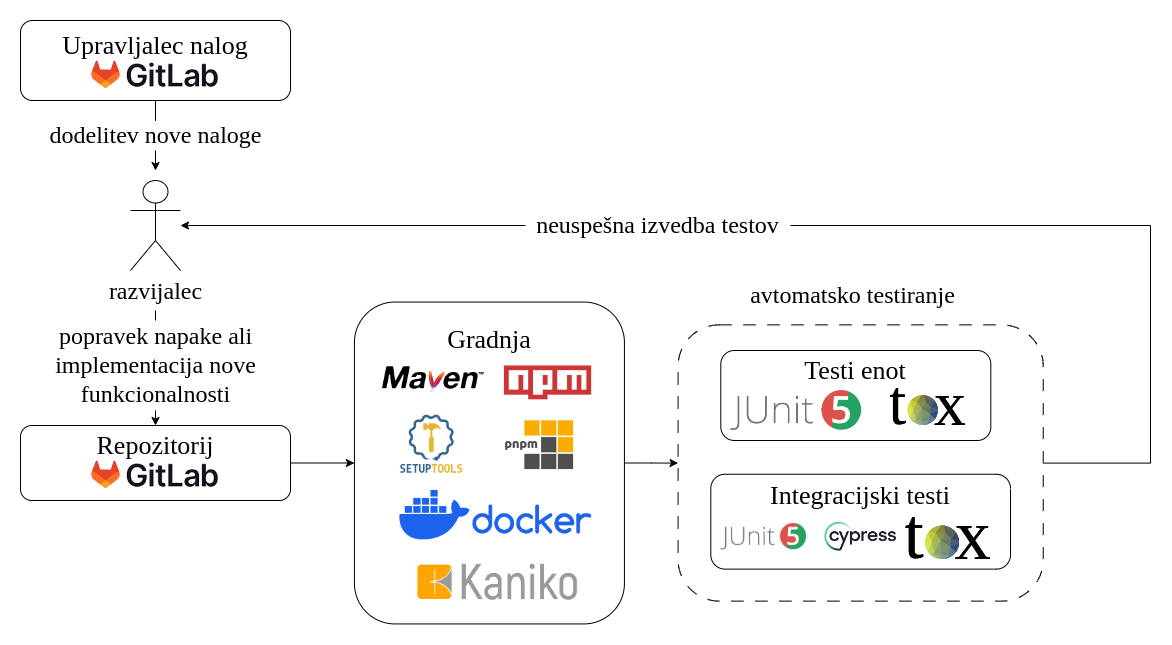
\includegraphics[width=13.5cm]{figures/diagram-neprekinjene-integracije-2.png}
    \end{center}
\caption{Diagram neprekinjene integracije.}
\label{fig:diagram-neprekinjene-integracije}
\end{figure}

\subsection{Testi enot}
\label{subsec:testi-enot}
Testi enot so testi, ki preverjajo posamezne enote ali skupine odvisnih enot programske opreme. Namen testov enot je pokazati, da programska koda naredi kar je bilo določeno v specifikaciji programske opreme. Razvijalci napišejo teste enot tako, da definirajo vhodne podatke posamezne enote in preverijo ali vrnejo pravilne rezultate, če predpostavimo, da vsi ostali deli sistema delujejo pravilno. Zato je za razvoj takšnih testov pogosto potrebna predpriprava okolja in ponarejanje rezultatov klicev funkcij, ki niso del trenutno testirane enote~\cite{Runeson2006}.

Za razvoj testov enot se pogosto uporabljajo knjižnice kot so: \textit{JUnit}\footnote{https://junit.org/junit5/}, \textit{pytest}\footnote{https://docs.pytest.org/en/latest/} in \textit{cypress}\footnote{https://www.cypress.io/}. Medtem, ko se za izvajanje testov uporabljajo različna orodja kot so: \textit{Maven}, \textit{Tox}, \textit{npm} in \textit{pnpm}.

\subsection{Integracijski testi}
\label{subsec:integracijski-test}
Integracijski testi so testi, ki testirajo delujoč program. Testi se izvajajo nad moduli namesto nad posameznimi enotami, kot pri testih enot. Cilj integracijskih testov je postaviti posamezne enote v njihovo predvideno okolje in čim bolj celovito preizkusiti njihove medsebojne interakcije~\cite{Leung1990, Delmaro2001}. Primera takšnih testov sta preverjanje interakcije z bazo in testiranje interakcije med mikroservisi. Ponavadi se tudi dalj časa izvajajo, saj je za izvajanje testov potrebno namestiti posamezne dele aplikacije.

\subsection{Razlogi za neprekinjeno integracijo}
Ko razvijalec želi dodati nekaj novega v programsko kodo aplikacije, si v svojem okolju ustvari kopijo temeljne programske kode, ki je v tistem trenutku aktualna. Medtem, ko razvijalec v svojem okolju razvija nove funkcionalnosti ali pripravlja popravke, lahko ostali razvijalci spreminjajo temeljno programsko kodo. Tako se lokalna kopija razvijalca čedalje bolj razlikuje od temeljne programske kode. Ostali razvijalci lahko v temeljno programsko kodo dodajo nove funkcionalnosti, nove knjižnice ali druge vire, ki lahko ustvarijo dodatne odvisnosti in potencialne konflikte. Dalj časa kot razvijalec svoje lokalne kopije ne združi s temeljno programsko kodo, večje je tveganje integracijskih konfliktov in napak pri združevanju kode~\cite{Duvall2007}. Preden razvijalec svoje spremembe doda v glavno vejo, mora najprej posodobiti svojo lokalno kopijo, da pridobi vse spremembe, ki so bile v vmesnem času dodane v glavno vejo. Več kot je bilo sprememb dodanih v vmesnem času, več dela ima razvijalec, preden svoje spremembe lahko doda v glavno vejo. Če razvijalec predolgo odlaša z oddajo kode, se njegova kopija lahko zelo razlikuje od kode v glavni veji in za integracijo svoje kode porabi več časa, kot ga je za razvoj sprememb. Temu rečemo tudi integracijski pekel~\cite{Cunningham2009}. Zato je ključno, da so naloge primerno razdeljene in smiselno umeščene v časovnico projekta.

Vpeljava neprekinjene integracije lahko prinese številne koristi pri razvoju programske opreme, vključno z izboljšano kakovostjo kode, hitrejšim objavljanjem posodobitev in zmanjšanjem tveganja napak pri integraciji in objavi. Vendar pa vpeljava neprekinjene integracije predstavlja tudi nekaj izzivov, kot je potreba po namestitvi in vzdrževanju infrastrukture za neprekinjeno integracijo in potreba po zagotavljanju učinkovitega postopka preizkušanja programske kode. 

\section{Neprekinjena dostava}
\label{sec:neprekinjena-dostava}

Neprekinjena dostava je metoda razvoja in izdelave, ki temelji na stalnem izboljševanju procesov in izdelkov ter zagotavljanju neprekinjene dostave izdelkov ali storitev. To pomeni, da se procesi in izdelki izboljšujejo in nadgrajujejo neprekinjeno ter dostava izdelkov ali storitev ne povzroči prekinitev ali zastoja v procesu. 

Cilj neprekinjene dostave je zmanjšanje časa med pisanjem kode in njene dostave končnim uporabnikom, obenem pa zagotavljanje visoke kakovosti in zanesljivosti. Neprekinjena dostava ima zato širši pomen, ki vključuje neprekinjeno integracijo in avtomatsko testiranje, obenem pa tudi izdajanje novih različic in avtomatsko objavo aplikacije v testno ali produkcijsko okolje. Pomemben del pa je tudi sistem za spremljanje napak in težav z zmogljivostjo, ki razvojni ekipi pošilja povratne informacije o delovanju aplikacije in jim na ta način pomaga identificirati in odpraviti napake~\cite{Humble2010}.

\subsection{Dostava izvorne kode}
\label{subsec:dostava-izvorne-kode}
Ključni del neprekinjene dostave je tudi dostava izvorne kode naročniku ali končnim uporabnikom. Proces prenosa kode mora biti dobro zasnovan, da zagotovimo, da se izvorna koda pravilno in učinkovito prenese. Dostava izvorne kode sicer ni nujna za vsak projekt in je odvisna od pogodbe med podjetjem in naročnikom ter poslovnega modela podjetja, ki je kodo napisalo. Vseeno pa se večkrat izkaže kot pomembna zahteva pri poslovno kritičnih aplikacijah, ker so bistvene za poslovanje podjetja in si zato podjetje želi ostati neodvisno od podjetja, ki je kodo napisalo.

Dostava izvorne kode naročniku je lahko koristna tako za naročnika kot tudi za podjetje, ki je napisalo izvorno kodo. Za naročnika je koristna, ker ni več odvisna od podjetja iz vidika posodobitev, vzdrževanja in podpore, vendar za to lahko najame drugo podjetje ali pa ta del prevzame sama. To se izkaže zelo uporabno predvsem takrat, ko podjetje, ki je ustvarilo izvorno kodo, preneha s svojim poslovanjem ali pa ni zmožno zagotoviti podpore. Dostava izvorne kode pa je smiselna tudi za podjetje, ki je izvorno kodo naredilo predvsem iz dveh vidikov~\cite{Humble2010}:
\begin{itemize}
    \item Prenos odgovornosti: z dostavo izvorne kode naročniku lahko podjetje prenese del odgovornosti vzdrževanja programske opreme na naročnika. To je še posebej koristno, če naročnik načrtuje prilagoditve ali spremembe programske opreme, saj podjetje ni odgovorno za morebitne težave ali napake, ki bi lahko nastale zaradi teh sprememb.
    \item Zmanjšanje bremena vzdrževanja in podpore: če ima naročnik dostop do izvorne kode, lahko sama odpravi težave in jih popravi, namesto, da bi se zanašala na podjetje za podporo.
\end{itemize}

Največji izziv pri tovrstni dostavi izvorne kode naročniku, pa je reproducibility... Izkaže se da ob razvoju knjižnic z orodji za gradnjo (kot je npm) preverja hash paketa ob vključevanju teh knjižnic v aplikacijo. Če izdamo tukaj mi to in naročniku oddamo tudi package-json-lock, se mora sha ujemati. Gradnja ne sme vsebovati timestampov, sha-jev od git commita ... 


\subsection{Neprekinjena namestitev}
\label{subsec:neprekinjena-namestitev}
Najširši obseg pa predstavlja neprekinjena namestitev, ki je praksa razvoja programske opreme, pri kateri se spremembe kode avtomatsko zgradijo, preizkusijo, oddajo naročniku in tudi objavijo v produkcijsko okolje brez posredovanja človeka. Predstavlja še en korak naprej od neprekinjene dostave, pri kateri se koda zgradi in preizkusi, vendar jo mora človek ročno objaviti v produkcijo.

Cilj neprekinjene namestitve je, da se nove funkcionalnosti in popravki čim hitreje dostavijo končnim uporabnikom. Da bi to dosegli, uporabljamo neprekinjeno integracijo, neprekinjeno dostavo in prakse neprekinjene namestitve, kot je proces upravljanja in rezervacije računalniških virov z uporabo datotek, ki jih računalnik zna prebrati - infrastruktura kot koda. Eno izmed takšnih tehnologij predstavlja platforma Kubernetes, ki smo jo sami uporabili in nam omogoča, da v formatu YAML (ang. YAML Ain't Markup Language) definiramo konfiguracijo namestitve naše aplikacije in jo s preprostim ukazom tudi namestimo. Neprekinjena namestitev lahko pomaga podjetju, da pogosteje objavi nove funkcionalnosti in posodobitve in izboljša učinkovitost in hitrost razvojnega procesa aplikacije~\cite{Wittig2016, Humble2014}.

\begin{figure}
    \begin{center}
        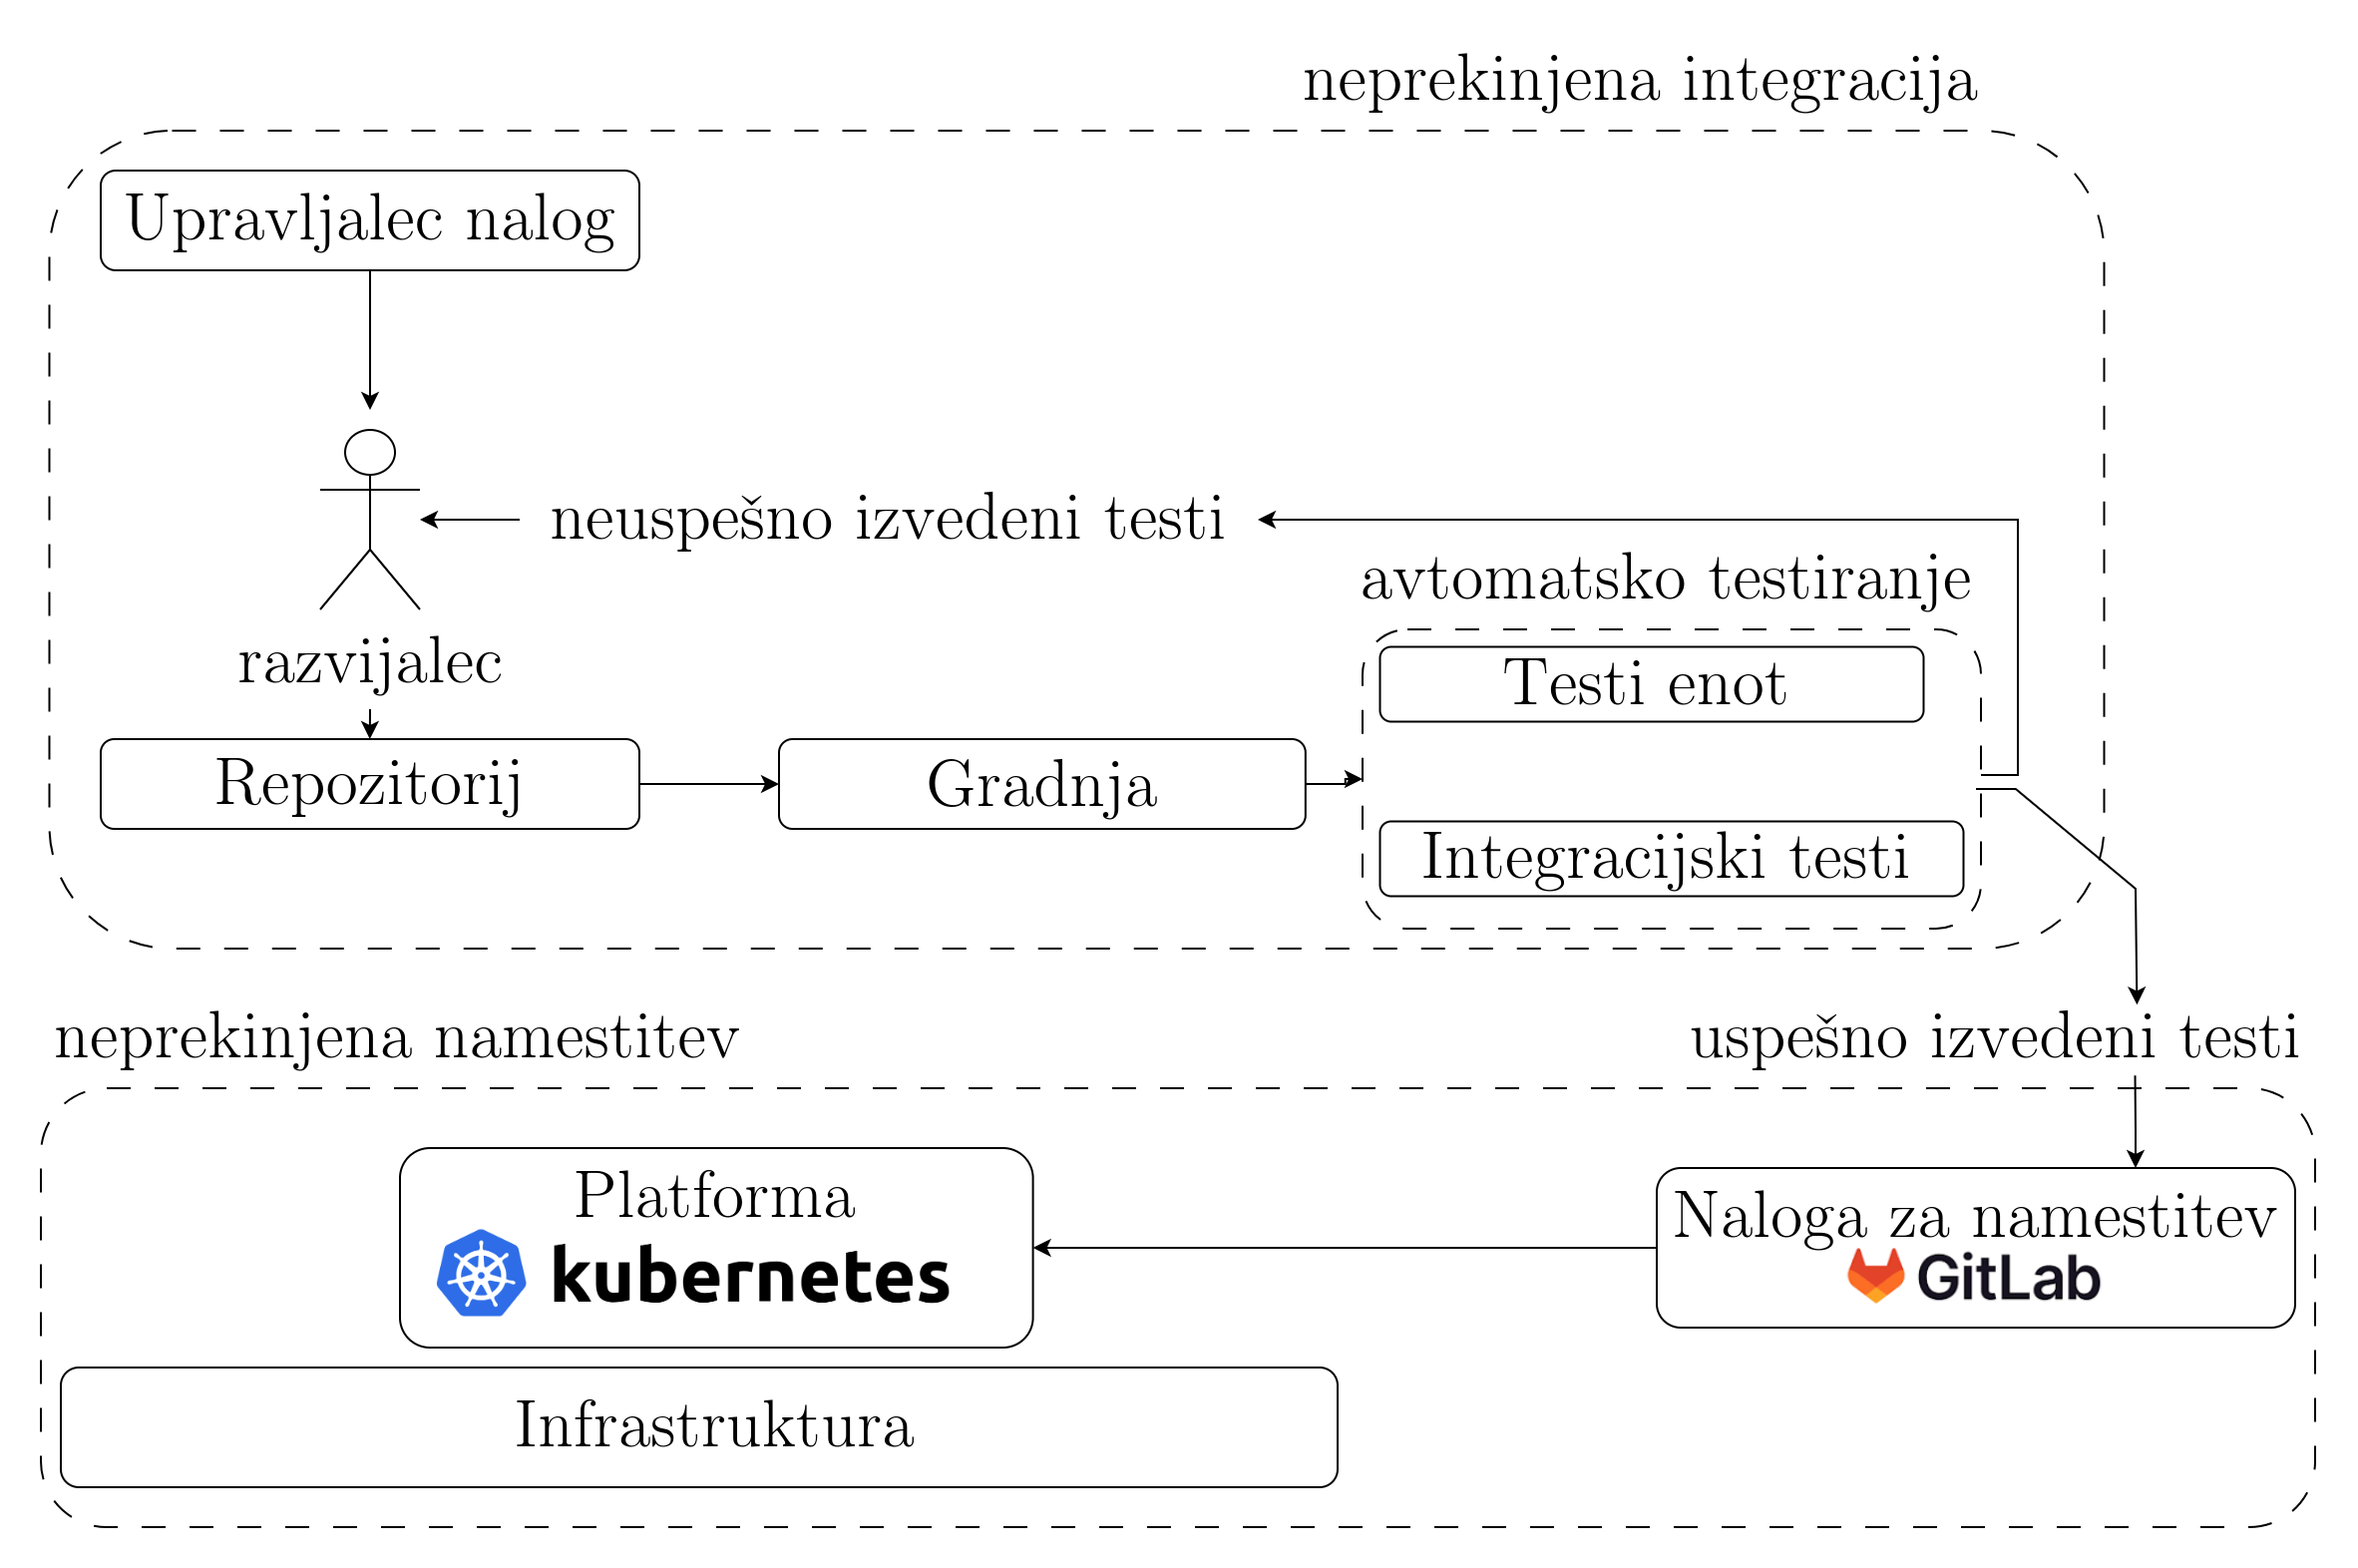
\includegraphics[width=13.5cm]{figures/diagram-neprekinjene-namestitve.png}
    \end{center}
\caption{Diagram neprekinjene integracije in namestitve.}
\label{fig:diagram-neprekinjene-integracije-in-namestitve}
\end{figure}

% Programerjem omogoča testiranje aplikacije v živo? Quality assurance?

\section{Organizacija projekta}
\label{sec:organizacija-projekta}
Struktura projekta opisuje kako je projekt organiziran in razmerja med različnimi deli projekta. Dobro strukturiran projekt pripomore k boljšemu razumevanju, vzdrževanju in razvijanju programske kode projekta. Obstaja veliko načinov strukturiranja projektov, seveda pa je struktura projekta odvisna od specifičnih potreb in ciljev projekta. Pri strukturiranju projekta so ključni deli:
\begin{itemize}
    \item Struktura imenika: Opisuje kako so datoteke in imeniki razporejeni na datotečnem sistemu. Dobra struktura imenika združuje odvisne datoteke in vire ter olajša iskanje datotek.
    \item Moduli in odvisnosti: V večini projektov je programska koda logično razdeljena na več modulov ali komponent, kjer je vsak izmed modulov zadolžen za le en del projekta. Ti moduli so lahko tudi odvisni med sabo, zato jih je potrebno skrbno organizirati in poskrbeti, da ne pride do krožnih odvisnosti.
    \item Skripti za gradnjo in namestitev projekta: Skripti opisujejo, kako projekt zgraditi in namestiti na testno in produkcijsko okolje. Ti skripti so po navadi del neprekinjene namestitve in morajo zato biti dobro organizirani in enostavni za razumevanje.
    \item Dokumentacija: Dobra dokumentacija je pomemben del vsakega projekta. Ta lahko vključuje uporabniška navodila, dokumentacijo aplikacijskega programskega vmesnika (ang. Application programming interface - API) in druge dokumente, ki pomagajo razvijalcem pri razvoju ter uporabnikom pri razumevanju delovanja projekta.
\end{itemize}

Na projektno strukturo močno vpliva tudi sistem za spremljanje različic kode, ki ga uporabljamo, saj lahko kodo shranjujemo v enem skupnem ali pa jo razdelimo v več ločenih repozitorijev. Izbira repozitorijske strukture je ključna za strukturo projekta, saj ima vsaka repozitorijska struktura svoje prednosti in slabosti. Najbolj pogosti repozitorijski strukturi sta: \textit{monorepo} in \textit{polirepo}~\cite{Wiki_Architectural_pattern, Kokrehel2022}.

\subsection{Monorepo}
\label{subsec:monorepo}
Monorepo ali monolitni repozitorij je poimenovanje organizacije in upravljanje različic izvorne kode z enim repozitorijem. Ta lahko vsebuje več projektov, paketov ali modulov in razvijalcem omogoča širok dostop do izvorne kode, skupnih orodji in skupne množice odvisnosti na enem mestu. Vizualizacijo takšne organizacije lahko vidimo na sliki \ref{fig:monorepo}. Prednosti monolitnega repozitorija so~\cite{Jaspan2018, Shakikhanli2022}:
\begin{itemize}
    \item Boljša preglednost izvorne kode: Razvijalci lažje najdejo relevantno dokumentacijo, primere implementacij in uporabe, kar pozitivno vpliva na hitrost razvijanja in kakovost kode. 
    \item Enostavne odvisnosti: Vsi paketi in moduli v repozitoriju imajo lahko enako različico in ni potrebno skrbeti katere različice so med seboj kompatibilne.
    \item Lažje spreminjanje odvisnih delov kode: Pri popravljanju in posodabljanju kode lahko popravimo vse dele kode, ki so med seboj odvisni in vse skupaj oddamo v repozitorij kot eno spremembo.
\end{itemize}

\begin{figure}
    \begin{center}
        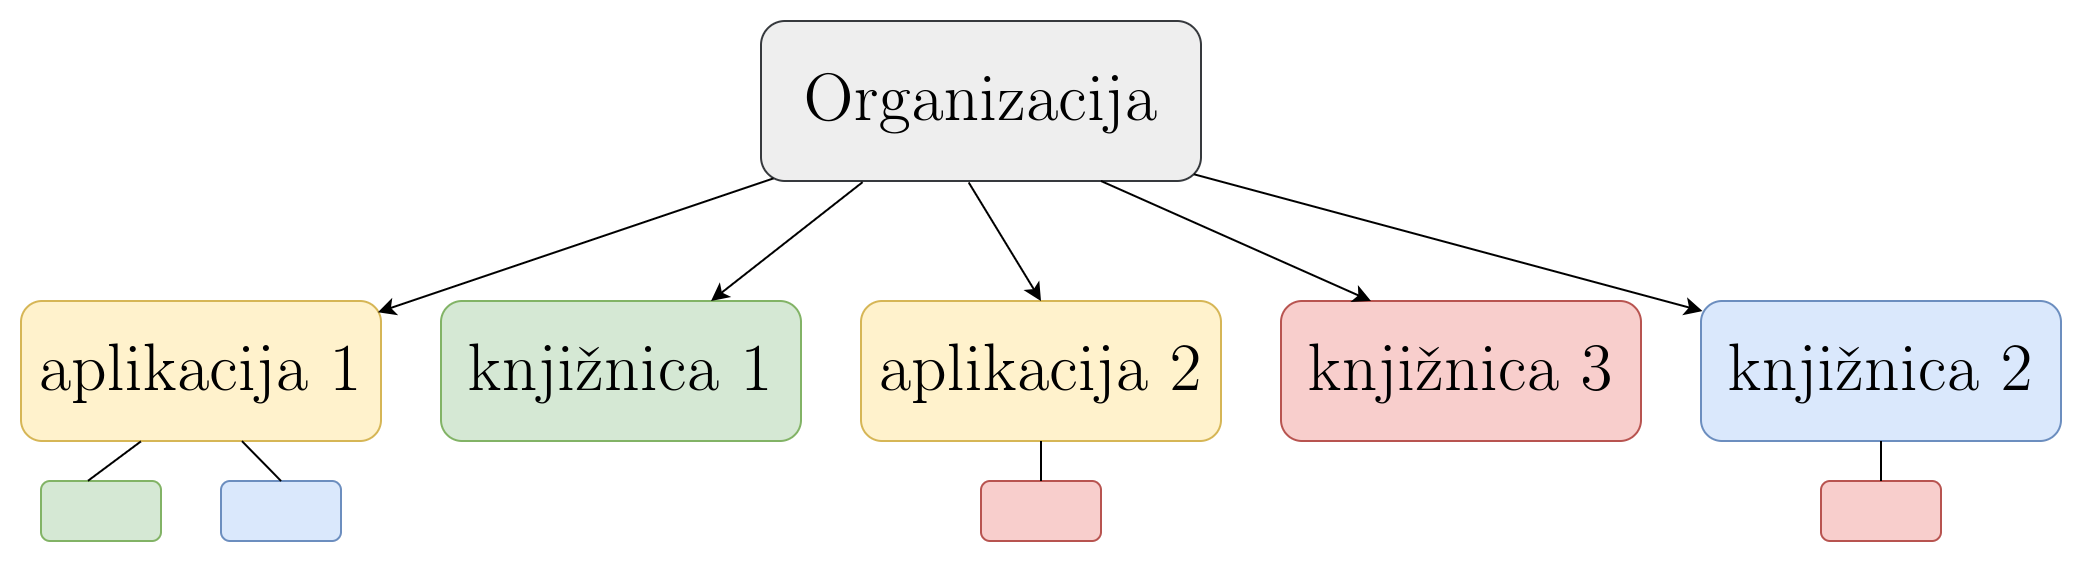
\includegraphics[width=12.5cm]{figures/monorepo.png}
    \end{center}
\caption{Vizualizacija organizacije z načinom monorepo.}
\label{fig:monorepo}
\end{figure}

Slabosti monolitnega repozitorija so~\cite{Harry2017}:
\begin{itemize}
    \item Velikost repozitorija: Monolitni repozitorij lahko skozi razvoj zasede veliko prostora na podatkovnem sistemu. To lahko oteži prenos izvorne kode iz repozitorija in ostale operacije sistema za upravljanje različic.
    \item Kompleksen cevovod za neprekinjeno dostavo: Kompleksnost konfiguracije cevovoda za neprekinjeno dostavo se poveča, saj je potrebno vse korake izvesti na vseh modulih in projektih. Da ohranimo učinkovitost, pa nočemo vedno izvajati vseh korakov za vse module, saj to podaljša izvajanje cevovoda.
    \item Veliki zahtevki za združitev vej: Ker repozitorij vsebuje vse odvisne dele kode, je ob posodobitvah lahko posodobljenih veliko vrstic izvorne kode. To lahko povzroči slabo preglednost sprememb v pregledu sprememb zahtevka za združitev.
    \item Orodja za upravljanje: Za učinkovito upravljanje monolitnega repozitorija so velikokrat potrebna dodatna programska orodja, kot so orodja za gradnjo aplikacije in upravitelji paketov. To lahko poveča kompleksnost razvijanja aplikacije.
\end{itemize}

\subsection{Polirepo}
\label{subsec:polirepo}
Polirepo je poimenovanje organizacije in načina upravljanja z različicami izvorne kode z več repozitoriji. Ti vsebujejo vse pakete in komponente izvorne kode, ki skupaj tvorijo celotno aplikacijo. Prednosti uporabe več repozitorijev so~\cite{Shakikhanli2022}:
\begin{itemize}
    \item Poenostavljeno upravljanje: S posameznimi moduli ali paketi v ločenih repozitorijih je lažje slediti spremembam in ugotoviti, katere spremembe spadajo k posameznim projektom.
    \item Ločitev odgovornosti: Shranjevanje posameznih projektov v ločenih repozitorijih lahko pomaga izolirati kodo in zmanjša tveganje za nastanek sporov med različnimi deli projekta.
    \item Fleksibilnost: ločeni repozitoriji omogočijo različnim ekipam razvijalcev, da se posvetijo vsak svojemu delu projekta brez medsebojnih motenj.
    \item Velikost repozitorijev: Ker je celoten projekt razdeljen na več repozitorijev, so ti repozitoriji manjši in zato lažji za prenos in delo na lokalnih računalnikih, še posebej, če razvijalec dela samo na enem delu projekta.
    \item Potencialno hitrejše gradnje: S posameznimi moduli ali paketi v ločenih repozitorijih jih je morda mogoče graditi neodvisno, kar lahko skrajša skupni čas gradnje.
\end{itemize}

\begin{figure}
    \begin{center}
        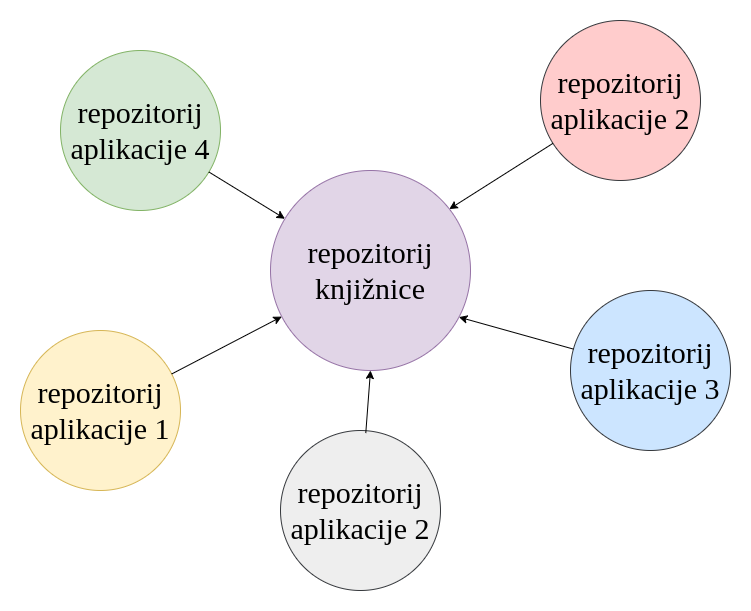
\includegraphics[width=9cm]{figures/polirepo.png}
    \end{center}
\caption{Vizualizacija organizacije z načinom polirepo.}
\label{fig:polyrepo}
\end{figure}

Slabosti uporabe več repozitorijev so~\cite{Shakikhanli2022}:
\begin{itemize}
    \item Upravljanje različic in določevanje odvisnosti: Potrebno je določiti, kako se bodo spreminjale različice modulov ali paketov v posameznih repozitorijih in kako bodo določene odvisnosti med njimi.
    \item Oteženo spreminjanje odvisnih delov kode: Po spremembi enega dela kode, se velikokrat zgodi, da je potrebno popraviti še kodo v odvisnih modulih ali paketih. To pomeni, da je treba v vsakem izmed odvisnih repozitorijev dodati spremembo in mogoče popraviti tudi številko različice.
\end{itemize}

Oba pristopa imata prednosti in slabosti in tisto, kar en razvijalec šteje za prednost, lahko drugemu predstavlja slabost. Na primer, nekateri razvijalci lahko vidijo enostavnost upravljanja enega samega repozitorija kot prednost uporabe monolitnega repozitorija, medtem ko drugi lahko zaradi potencialne povečane zapletenosti vidijo to kot slabost. Podobno lahko nekateri razvijalci vidijo sposobnost enostavnega deljenja kode in virov med projekti kot prednost uporabe več repozitorijev, medtem ko drugi lahko vidijo potrebo po upravljanju več repozitorijev kot slabost. Zato je izbira med uporabo monolitnega repozitorija ali več repozitorijev največkrat stvar osebnega okusa in je odvisna od specifičnih potreb ter narave projekta kot tudi delovnih navad podjetja.

\section{Vrsta projekta}
\label{sec:vrsta-projekta}
V poglavju bomo predstavili dve vrsti projektov: aplikacije in knjižnice. Razlikovanje je pomembno, ker vrsta projekta vpliva na cevovod CI/CD, ki se za razvoj projekta uporablja.

\subsection{Aplikacija}
\label{subsec:aplikacija}
Aplikacije so samostojno izvršljivi programi, ki so zasnovani za izvajanje določenih nalog ali zagotavljanje posebnih fukcionalnosti končnim uporabnikom. Uporabniki lahko aplikacije uporabljajo preko spletnih strežnikov, ki aplikacije strežejo, namestitve aplikacije na osebni računalnik, namestitve aplikacije na mobilni telefon in druge načine. Zato je programsko kodo aplikacije potrebno ustrezno pripraviti tudi za namestitev v končno okolje. Primeri aplikacij so: računalniške igre, zaledni strežniki, čelne aplikacije, orodja za urejanje besedil, integrirana razvojna okolja in podobno.

\subsection{Knjižnica}
\label{subsec:knjižnica}
Knjižnice so zbirke vnaprej napisanih programskih modulov, funkcij in razredov, ki jih razvijalci lahko večkrat uporabijo, da si olajšajo razvoj aplikacij. Knjižnic končni uporabniki neposredno ne uporabljajo in jih zato ni potrebno namestiti v končna okolja. Da pa lahko razvijalci knjižnice uporabijo za razvoj aplikacije, pa jih je potrebno naložiti na repozitorij iz katerega lahko orodja za gradnjo ob gradnji aplikacije knjižnice prenesejo. Primeri knjižnic so: knjižnice za delo z grafičnimi vmesniki, knjižnice za izračun matematičnih funkcij, knjižnice za izvajanje spletnih zahtevkov in podobno.

%----------------------------------------------------------------
% Poglavje 3 - Tehnologije
%----------------------------------------------------------------

\chapter{Uporabljene tehnologije in aplikacije}
\label{ch:uporabljene-tehnologije-in-aplikacije}
V tem poglavju bomo predstavili tehnologije in aplikacije, ki so bile uporabljene za postavitev cevovoda neprekinjene integracije in dostave. Opisali bomo repozitorije za nadzor različic in orodja za gradnjo, ki so bila uporabljena, pa tudi aplikacijo GitLab in konfiguracijski strežnik. Prav tako bomo podrobneje obravnavali način zagotavljanja varnosti aplikacije in opisali pomožna orodja in njihov namen.

\section{Repozitoriji za nadzor različic}
\label{sec:repozitoriji-za-nadzor-različic}
Za razvoj aplikacij uporabljamo več repozitorijev, ki služijo različnim namenom. Izvorna koda se nahaja v repozitoriju s sistemom za nadzor različic, ki razvijalcem omogoča preprost pregled sprememb kode in združevanje sprememb iz različnih vej. Interne knjižnice, od katerih so aplikacije odvisne, so v obliki artefaktov ali paketov naložene v repozitorij, katerega upravlja centralni upravitelj repozitorijev. Aplikacije po gradnji največkrat zapakiramo v vsebniško sliko, ki so shranjene v registru vsebniških slik. V nadaljevanju predstavimo, katere implementacije posameznih repozitorijev smo uporabili pri implementaciji cevovoda za neprekinjeno integracijo in dostavo.

\subsection{Git}
\label{subsec:git}
Git\footnote{\url{https://git-scm.com/}} je sistem za upravljanje različic, ki se pogosto uporablja pri razvoju programske opreme. Omogoča, da več razvijalcev naenkrat dela na enaki izvorni kodi in jim pomaga slediti spremembam, ki so bile narejene~\cite{loeliger2012version}.

Uporaba sistema za upravljanje različic Git deluje tako, da ima vsak razvijalec kopijo celotnega repozitorija na svojemu računalniku vključno z vso zgodovino vseh sprememb, ki so bile narejene na izvorni kodi. Ko razvijalec razvija aplikacijo, spreminja zgolj kodo, ki jo ima shranjeno na svojem računalniku. Če želi spremembe oddati na oddaljen repozitorij, mora svoje spremembe s potrditvijo najprej dodati v svoje lokalno skladišče, nato pa jih lahko naloži še na oddaljen repozitorij~\cite{loeliger2012version}.

Drugi razvijalci lahko nato prenesejo spremembe iz oddaljenega repozitorija v svoje lokalno skladišče in združijo spremembe s svojo kopijo. Če so na oddaljenem repozitoriju nove spremembe kode na enakih delih kot spremembe v skladišču razvijalca, mora razvijalec, ki želi združiti kodo s svojo lokalno kopijo, izbrati katere spremembe bo obdržal. Git vsebuje orodja, ki ta postopek združevanja poenostavijo~\cite{loeliger2012version}.

Za neprekinjeno integracijo in dostavo aplikacij je Git pomemben predvsem zaradi sistema za sledenje spremembam, ki omogoča, da celotna ekipa razvijalcev naenkrat sodeluje pri razvoju. Pri neprekinjeni integraciji je zelo pomembno, da lahko hitro in enostavno zaznamo in testiramo spremembe, ki so bile narejene, kot tudi, da lahko združimo spremembe. Hkrati omogoča, da v primeru napak pri testiranju ali drugih težav enostavno in hitro vrnemo aplikacijo na zadnje delujoče stanje~\cite{Dingare2022}.

\subsection{Nexus}
\label{subsec:nexus}
Apache Nexus\footnote{\url{https://www.sonatype.com/products/nexus-repository}} je eden od najbolj priljubljenih odprtokodnih upravljalcev repozitorijev, ki se uporabljajo za gostovanje in upravljanje artefaktov, kot so datoteke tipa JAR in ostale binarne komponente, ki jih projekti potrebujejo za svojo gradnjo in delovanje. Poleg strežbe repozitorijev z interno razvitimi artefakti, se pogosto uporablja kot nadomestni strežnik za zunanje repozitorije, kot je na primer centralni repozitorij Maven\footnote{\url{https://mvnrepository.com/repos/central}}. Takšen način uporabe zmanjša število zunanjih odvisnosti, ki jih je potrebno prenesti s spleta, pohitri gradnjo aplikacij in izboljša njihovo varnost z nadzorom artefaktov, ki so na voljo. Slednje omejuje z nastavljivimi pravili, kot npr. da morajo biti vsi artefakti digitalno podpisani ali pa da morajo biti odobreni s strani administratorja~\cite{Varanasi2019}.

Nexus ponuja tudi uporabniški vmesnik, s katerim je enostavno poiskati in prenesti artefakte kot tudi ročno naložiti nove artefakte v repozitorij. Prav tako izpostavlja aplikacijski programski vmesnik z arhitekturnim slogom REST, ki se lahko uporablja za avtomatizacijo podobnih opravil. Za proces neprekinjene integracije in dostave aplikacij je Nexus pomemben zaradi več razlogov:
\begin{itemize}
    \item Pomaga poenotiti proces razvijanja aplikacije tako, da nudi enotno in konsistentno mesto za shranjevanje zgrajenih artefaktov.
    \item Poveča učinkovitost in hitrost z zagotavljanjem hitrega in zanesljivega načina dostopa do zgrajenih artefaktov.
    \item Izboljša varnost z nadzorom dostopa do artefaktov in dodatnimi pravili, ki omejujejo dostop.
    \item Olajša sledljivost s hranjenjem različnih različic artefaktov, ki so bili zgrajeni in nameščeni.
\end{itemize}

\subsection{Register vsebniških slik }
\label{subsec:register-vsebniskih-slik}
Register vsebniških slik je sistem za centralizirano hranjene in distribucijo vsebniških slik, ki so podrobneje predstavljene v poglavju \ref{subsec:docker}. Služi kot sistem za upravljanje različic slik, v kateremu lahko slike shranjujemo, jih delimo z drugimi in jih prenašamo~\cite{Anwar2018}.

Obstaja veliko javnih registrov do katerih dostop ni omejen, kot so: Docker Hub\footnote{\url{https://hub.docker.com/}}, ki je privzeti register in ga vzdržuje Docker, Quay\footnote{\url{https://quay.io/}} in IBM Cloud container registry\footnote{\url{https://www.ibm.com/cloud/container-registry}}. Na lastni infrastrukturi pa lahko postavimo tudi privatni register, do katerega omejimo dostop in s tem zagotovimo boljšo varnost~\cite{Anwar2018}.

V kontekstu neprekinjene integracije nam register slik vsebnikov omogoča hranjenje vsebniških slik, ki jih proces CI zgradi. Te slike lahko potem uporabimo za postavitev testnega okolja pred oddajo v produkcijo. V kontekstu neprekinjene dostave pa nam register omogoča upravljanje z različicami aplikacijskih vsebniških slik in v primeru težav hitro vračanje aplikacije na predhodno delujočo in preverjeno različico.

\section{Orodja za gradnjo}
\label{sec:orodja-za-gradnjo}
V tem poglavju bomo predstavili orodja za gradnjo aplikacij razvitih v programskih jezikih Java, Python, JavaScript in TypeScript in orodji za gradnjo vsebniških slik, ki smo jih v cevovodu neprekinjene integracije in dostave uporabili.

\subsection{Maven}
\label{subsec:maven}

Maven\footnote{\url{https://maven.apache.org/}} je orodje za avtomatizacijo gradnje, testiranja in namestitve projektov napisanih v programskem jeziku Java. Uporablja deklarativen pristop, s katerim razvijalci naštejejo vse odvisnosti, vtičnike in ostale informacije, potrebne za gradnjo projekta, v datoteko \texttt{pom.xml}~\cite{Varanasi2019}.

Orodje je pomembno za neprekinjeno integracijo in dostavo aplikacij, ker omogoča konsistenten in ponovljiv način gradnje, testiranja in nameščanja aplikacije. Z orodjem lahko razvijalci opišejo vse potrebne korake za gradnjo projekta v eni konfiguracijski datoteki, ki jo v procesu CI/CD lahko nato uporabimo za avtomatizacijo gradnje in namestitve projekta.

\subsection{Gradle}
\label{subsec:gradle}
Gradle\footnote{\url{https://gradle.org/}} je prav tako kot Maven odprtokodno orodje za gradnjo projektov, vendar je bolj fleksibilno. Tako kot Maven, se tudi Gradle primarno uporablja za projekte spisane v programskem jeziku Java, vendar se lahko uporablja tudi za gradnjo projektov v drugih programskih jezikih, kot na primer C++ ali Python. Za definicijo skripta za gradnjo projekta uporablja domensko-specifičen jezik, ki je osnovan na jeziku Groovy in omogoča bolj zgoščene in ekspresivno napisane skripte, v primerjavi s skripti v formatu XML, ki ga uporablja Maven~\cite{Ikkink2015}.

Podobno kot Maven, je Gradle pomemben za neprekinjeno integracijo in dostavo aplikacije, ker omogoča avtomatizacijo gradnje in namestitve projekta. Gradle podpira tudi gradnjo več projektov hkrati in inkrementalno gradnjo ter je zato primeren tudi za velike in kompleksne projekte. Znan je tudi po svojem sistemu predpomnenja, ki z beleženjem vhodov in izhodov gradnje ter njihovo ponovno uporabo, pohitri gradnjo projekta. To je še posebej uporabno za proces CI/CD, kjer želimo projekt zgraditi čim hitreje.

\subsection{Node Package Manager ali NPM}
\label{subsec:npm}

Node Package manager\footnote{\url{https://www.npmjs.com/}} je orodje za upravljanje paketov, ki so napisani v programskem jeziku JavaScript ali TypeScript in se uporabljajo v izvajalnem okolju Node.js. Orodje je vključeno v namestitveni paket izvajalnega okolja Node.js in je avtomatsko nameščeno ob namestitvi Node.js, zato služi kot privzeti upravitelj paketov. Uporablja se v ukazni vrstici in razvijalcem omogoča enostavno namestitev, upravljanje in deljenje paketov. V datoteki \texttt{package.json} razvijalci določijo odvisnosti, ki jih projekt zahteva. Te odvisnosti nato enostavno namestijo z uporabo orodja NPM, ki avtomatsko poišče ustrezne pakete in jih prenese iz registra NPM ali iz drugih virov kot je npr. repozitorij Nexus. Prav tako omogoča upravljanje različič paketov, posodabljanje paketov, odstranjevanje paketov in objavljanje lastnih paketov v zasebne ali javne repozitorije. Poskrbi tudi za razreševanje odvisnosti in zagotavlja, da so vsi zahtevani paketi in njihove odvisnosti pravilno nameščeni in združljivi med seboj~\cite{Ali2013}.

\subsection{Performant Node Package Manager ali PNPM}
\label{subsec:pnpm}
Performant Node Package Manager\footnote{\url{https://pnpm.io/}} je alternativa orodju NPM, ki si prizadeva izboljšati efektivnost in učinkovitost namestitve in upravljanja paketov. Za razliko od orodja NPM, ki uporablja centralen predpomnilnik paketov in namešča odvisnosti projekta v mapo poimenovano \texttt{node\_modules}, PNPM uporablja virtualno shrambo. Namesto podvajanja odvisnosti za več projektov, jih shrani na centralno mesto na datotečnem sistemu, kar omogoča, da si različni projekti odvisnosti delijo. Na ta način izboljšuje hitrost namestitve in zmanjšuje prostor, ki ga posamezni projekti zasedajo. Prav tako omogoča hitrejše in učinkovitejše posodobitve paketov, saj je ob posodobitvi potrebno posodobiti samo eno kopijo paketa v centralni virtualni shrambi. Orodje je združljivo z obstoječimi projekti Node.js in ga lahko uporabimo kot zamenjavo za orodje NPM. Ponuja podobne ukaze in je zato tudi enostavno za uporabo~\cite{Jacobs2019, PnpmBenchmarks2023}.

\subsection{Pip Installs Packages ali PIP}
\label{subsec:pip}
Pip Installs Packages\footnote{\url{https://pypi.org/project/pip/}} je privzeto orodje za upravljanje paketov, ki so napisani v programskem jeziku Python. Omogoča enostavno namestitev, nadgradnjo in upravljanje s paketi, ki niso del osnovne knjižnice. Orodje omogoča razvijalcem enostaven dostop in namestitev paketov iz Python Package Index-a (PyPI), ki gostuje odprto-kodne pakete~\cite{Pip2023}. Seznam paketov, ki jih projekt potrebuje, prebere iz datoteke \texttt{requirements.txt}, ki v vsaki vrstici vsebuje ime paketa in njegovo verzijo.

\subsection{Setuptools}
\label{subsec:setuptools}
Setuptools\footnote{\url{https://pypi.org/project/setuptools/}} je knjižnica, ki poenostavi razvoj in distribucijo paketov v programskem jeziku Python. Vsebuje zbirko uporabnih funkcij in razširitev, ki nam pomagajo pri pakiranju, distribuciji in namestitvi paketov. Glavne funkcionalnosti so~\cite{Younker2008}:
\begin{itemize}
    \item Podpora za kreiranje paketov: knjižnica za konfiguracijo gradnje paketov in meta podatkov o paketu, kot so ime, različica, avtor, odvisnosti in vhodne točke uporablja datoteko \texttt{setup.py}. Na ta način razvijalcu omogoči, da definira strukturo projekta in določi vire in dodatne datoteke, ki so del projekta.
    \item Upravljanje odvisnosti: knjižnica s ključno besedo \texttt{requires} v konfiguracijski datoteki \texttt{setup.py} omogoča avtorjem paketa nastavitev odvisnosti, ki jih paket potrebuje. Knjižnica prav tako omogoča avtomatsko razrešitev in namestitev teh odvisnosti, kar poenostavi namestitev in uporabo paketa.
    \item Vstopne točke: knjižnica omogoča uporabo vhodnih točk, ki na standarden način definirajo, kako lahko ostali paketi in aplikacije razširijo funkcionalnosti paketa. Hkrati omogoča dinamično odkrivanje in namestitev vtičnikov brez navajanja eksplicitnih uvozov modulov s stavkom \texttt{import}.
    \item Integracija s PyPI: knjižnica je dobro integrirana s PyPI in vsebuje orodja za nalaganje paketov na PyPI.
    \item Razširitev osnovnih ukazov: osnovne ukaze razširja z ukazi, ki pomagajo pri gradnji različnih distribucij, ustvarjanju dokumentacije in zagonu testov.
\end{itemize}

\subsection{Docker}
\label{subsec:docker}
Docker\footnote{\url{https://www.docker.com/}} je odprtokodno orodje za razvoj, namestitev in zagon aplikacij z uporabo slik Docker ter njihovih vsebnikov (ang. \textit{container}). Slike Docker so način pakiranja aplikacij in njihovih odvisnosti, ki zagotavljajo, da jih lahko zanesljivo zaženemo v različnih okoljih in vsebujejo vse potrebno za zagon aplikacije: kodo, izvajalno okolje, knjižnice in sistemska orodja. Vsebniki pa so zagnani primerki slike Docker. Takšen standardiziran način pakiranja in distribucije aplikacij znatno olajša proces razvoja, nameščanja in upravljanja z aplikacijami. Glavne prednosti orodja Docker so~\cite{Rad2017}:
\begin{itemize}
    \item Prenosljivost: vsebniki so neodvisni od operacijskega sistema, lahko jih zaženemo na kateremkoli sistemu, ki podpira Docker in zagotavljajo konsistentno obnašanje v različnih okoljih.
    \item Skalabilnost: orodje Docker omogoča hitro razširljivost aplikacij s podvajanjem vsebnikov, ki izvajajo enako aplikacijo in porazdelitvijo obremenitve med njimi. 
    \item Izolacija: vsak vsebnik deluje v svojem izoliranem okolju, kar zagotavlja izolacijo procesov in preprečuje konflikte med aplikacijami.
    \item Učinkovita raba virov: vsebniki si delijo računalniške vire sistema, na katerem delujejo.
    \item Upravljanje različic: orodje Docker z označevanjem vsebniških slik omogoča enostavno upravljanje različic in vračanje na starejše različice.
\end{itemize}

\subsection{Kaniko}
\label{subsec:kaniko}
Kaniko\footnote{\url{https://github.com/GoogleContainerTools/kaniko}} je odprtokodno orodje za gradnjo vsebniških slik iz datotek Docker (ang. \textit{Dockerfile}) znotraj vsebnika ali na gruči Kubernetes. Za gradnjo vsebniških slik ne potrebuje privilegiranega dostopa do prikritega procesa Docker (ang. \textit{Docker daemon}), kar predstavlja glavno prednost pred načinom gradnje vsebniških slik, ki ga uporablja platforma Docker.

Platforma Docker za gradnjo slik uporablja prikriti proces, ki potrebuje korenski dostop in visoke pravice na gostujočem sistemu. Uporabniki v nekaterih okoljih, kot je na primer Kubernetes ali cevovod za neprekinjeno integracijo in dostavo zaradi varnostnih zahtev nimajo zahtevanih pravic za zagon prikritega procesa. Kaniko to težavo reši z uporabo samostojnega orodja, ki se zažene znotraj vsebnika in zgradi sliko brez priviligiranega dostopa. Vse potrebne operacije, kot so: prenos osnovnih slik, izvajanje ukazov za gradnjo slike in kreiranje končne slike vsebnika, izvede s pravicami, ki jih ima navaden uporabnik gostiteljskega sistema. To nam omogoča, da lahko zgradimo slike na gruči Kubernetes ali drugih platformah za orkestracijo~\cite{Kaniko2023}.

\section{GitLab}
\label{sec:gitlab}
GitLab\footnote{\url{https://about.gitlab.com/}} je spletna platforma za razvijalce in sistemske inženirje, ki vsebuje velik nabor orodji za upravljanje in dostavo aplikacij. Osnovni namen platforme je porazdeljen sistem za nadzor različic (ang. \textit{distributed version control system - DVCS}), v katerem lahko razvijalci gostijo svoje repozitorije izvorne kode, na podoben način kot v sistemu Git (\ref{subsec:git}), obenem pa vsebuje še veliko funkcionalnosti~\cite{GitLab2023}:
\begin{itemize}
    \item Orodja za vodenje projekta, ki olajšajo: organiziranje projekta, sledenje nalogam, dodeljevanje nalog razvijalcem in določanje mejnikov.
    \item Sistem za gradnjo in zagon cevovodov za neprekinjeno integracijo in dostavo aplikacij.
    \item Orodja za pregled kode in medsebojno sodelovanje, ki omogočajo: pregled kode, dodajanje komentarjev na posamezne vrstice v kodi, pregled zahtevkov za združitev in upravljanje vej.
    \item Vgrajen register za shranjevanje in upravljanje z vsebniki in njihovo uporabo v delovnih procesih.
    \item Varnostna preverjanja in preverjanja skladnosti kode z industrijskimi standardi.
    \item Možnost namestitve na lastni infrastrukturi ali v oblaku, kar omogoča skalabilnost in visoko razpoložljivost.
\end{itemize}

\subsection{Orodje GitLab CI/CD}
\label{subsec:orodje-gitlab-ci-cd}

GitLab CI/CD je orodje za gradnjo in zagon cevovodov za neprekinjeno integracijo in dostavo aplikacij, ki je integriran v platformo GitLab. Razvijalcem omogoča avtomatizacijo gradnje, testiranja in namestitve aplikacij in s tem olajša proces dostave programske opreme. Temelji na konceptu cevovodov, ki jih predstavljajo zaporedja nalog. Vsak cevovod ima lahko več faz v kateri je lahko več nalog, vsaka naloga pa ima lahko več akcij. Z razporejanjem nalog po fazah, zagotovimo pravilen vrstni red izvajanja nalog. Cevovode definiramo v konfiguracijski datoteki \texttt{.gitlab-ci.yml}, v formatu YAML, ki se mora nahajati v korenskem direktoriju projekta. V tej datoteki specificiramo tudi vse artefakte, ki jih naloge generirajo, odvisnosti in okoljske spremenljivke.

Za izvajanje nalog skrbijo izvajalci nalog GitLab. Izvajajo se lahko na lastni infrastrukturi ali na oblačnih virtualnih strojih in omogočajo paralelno izvajanje nalog, kar lahko znatno pohitri povprečen izvajalni čas cevovoda. Izvajalci nalog so različnih tipov glede na to, katerim projektom so na voljo:
\begin{itemize}
    \item deljeni: na voljo vsem projektom, ki obstajajo na instanci platforme GitLab,
    \item skupinski: na voljo samo projektom v specifični skupini in
    \item projektni: na voljo samo specifičnemu projektu.
\end{itemize}

Izvajalce nalog lahko prilagodimo svojim potrebam z omejitvijo števila vzporednih nalog, ki jih lahko izvajajo, omejitvami virov, ki so jim na voljo, in okoljskimi spremenljivkami. Lahko jim dodelimo tudi oznake, s katerimi lahko na nalogo natančno določimo njihovo izvajanje. Med posameznimi izvajalci nalog je zagotovljena izolacija, tako da se lahko naloge izvajajo neodvisno druga od druge. Hkrati je z nadzorom dostopa in ustreznimi metodami verodostojnosti, ki zagotavljajo integriteto celotnega procesa, poskrbljeno za varnost.

\section{Kubernetes}
\label{sec:kubernetes}
Kubernetes\footnote{\url{https://kubernetes.io/}} je odprtokodna rešitev za orkestracijo vsebnikov, ki avtomatizira namestitev, skaliranje instanc in upravljanje aplikacij nameščenih v vsebnikih. Glavni gradniki platforme Kubernetes so~\cite{Burns2022}:
\begin{itemize}
    \item Vozlišča (ang. nodes) - stroji, na katerih so nameščeni vsebniki. Izvajalno okolje vsakega vozlišča mora vsebovati orodja, ki so potrebna za upravljanje vsebnikov, kot je npr. platforma Docker.
    \item Stroki (ang. pods) - vozlišča gostijo stroke, kjer tečejo vsebniki, ki so komponente aplikacije. Vsebniki, ki tečejo na istem stroku si delijo omrežje, imenski prostor in prostor za hrambo podatkov.
    \item Nabori podvajanj (ang. replica set) - njihova naloga je ohraniti stabilen nabor kopiranih strokov.
    \item Storitve - abstrakcije, ki predstavljajo nabor strokov in definirajo način dostopa do njih. Omogočajo mehanizme za upravljanje z obremenitvijo in odkrivanje storitev.
    \item Ingress - objekti programskega vmesnika, ki upravljajo zunanji dostop do storitev v gruči. Omogočajo združevanje pravil usmerjanja v en sam vir in lahko izpostavijo več storitev pod istim naslovom IP.
    \item Shrambe podatkov (ang. volumes) - rezervirani podatkovni prostor na datotečnem sistemu, ki je neodvisen od življenjskega cikla vsebnikov in na ta način omogočajo dolgotrajno shrambo podatkov, tudi ob zaustavitvi ali ponovnem zagonu vsebnikov.
    \item Oznake in selektorji - oznake predstavljajo objekti v obliki ključ-vrednost, ki so dodani gradnikom platforme Kubernetes. Selektorji pa se uporabljajo za identifikacijo objektov na podlagi njihovih oznak.
    \item Namestitive (ang. deployments) - omogočajo upravljanje namestitve in posodobitev vmesnikov. Definiramo jih z deklarativno konfiguracijsko datoteko in skrbijo za ustrezno skaliranje, posodobitve brez zaustavitve (ang. rolling updates) in vračanje na starejše različice (ang. rollback).
\end{itemize}

% \section{Konfiguracijski strežniki}
% \label{sec:konfiguracijski-strežniki}

% \subsection{Konfiguracijski strežnik Spring Boot}
% \label{subsec:spring-boot-configuration-server}

% \section{Zagotavljanje varnosti}
% \label{sec:zagotavljanje-varnosti}

% \subsection{Kubernetes v izoliranem produkcijskem okolju}
% \label{subsec:kubernetes-v-izoliranem-produkcijskem-okolju}

% \section{Beleženje dogodkov in zbiranje metrik}
% \label{subsec:belezenje-dogodkov-in-zbiranje-metrik}

% \subsection{Graylog}
% \label{subsec:graylog}

% \subsection{Elastic}
% \label{subsec:elastic}

% \subsection{Kibana}
% \label{subsec:kibana}

\section{Zagotavljanje kakovosti kode}
\label{sec:zagotavljanje-kakovost-kode}
V tem poglavju bomo predstavili orodja za zagotavljanje kakovosti kode. To so orodja, ki naredijo statično analizo kode, kar pomeni, da kodo analizirajo brez zagona aplikacije, in nas opozorijo na znane pomanjkljivosti.

\subsection{SonarQube}
\label{sec:sonarqube}
SonarQube\footnote{https://www.sonarsource.com/products/sonarqube/} je odprtokodna platforma za avtomatsko preverjanje kakovosti kode z namenom zaznave napak, slabo napisane kode (ang. code smell) in varnostnih pomanjkljivosti v programski kodi. Podpira več kot 25 programskih jezikov in se uporablja v več kot 85000 organizacijah. Orodje deluje na osnovi pravil in konfiguracij, ki jih lahko tudi sami dodamo ter služijo kot standardi programske kode. V primeru da del kode krši katerega izmed pravil, nas orodje opozori na napako. Poleg že vgrajenih pravil, uporablja tudi pravila drugih popularnih orodji za preverjanje kakovosti kode kot sta \textit{FindBugs} in \textit{PMD}~\cite{Marcilio2019}.

Platforma je sestavljena iz orodji in programskih vtičnikov, ki jih lahko uporabimo za zagon analize kakovosti kode lokalno ali v cevovodu CI, ter spletnega vmesnika, ki prikazuje podrobna poročila in metrike kakovosti kode, kar razvojnim ekipam olajša spremljanje napredka in dodeljevanje nalog za izboljšanje kakovosti.

\subsection{ESLint}
ESLint\footnote{https://eslint.org/} je najbolj priljubljeno odprtokodno orodje za statično analizo programske kode, ki je napisana v programskih jezikih JavaScript, TypeScript ali ECMAScript. Orodje sestavlja 236 osnovnih pravil, ki jih razvijalci lahko poljubno vklopijo ali izklopijo in razvijalce opozarjajo na potencialno problematične dele kode~\cite{Tomasdottir2017}.

\section{Pomožne tehnologije}
\label{subsec:pomozne-tehnologije}
V tem poglavju bomo predstavili pomožne tehnologije, ki smo jih uporabili vzpostavitev cevovoda CI/CD. To so tehnologije, ki niso nujno potrebne vendar so nam olajšale razvoj in namestitev aplikacij.

\subsection{Konfiguracijski strežnik Consul}
\label{subsec:konfiguracijski-strežnik-consul}

Consul\footnote{\url{https://www.consul.io/}} je platforma za upravljanje s porazdeljenimi storitvami, ki omogoča odkrivanje storitev, upravljanje konfiguracije in preverjanje zdravja storitev~\cite{Sabharwal2021}.

Ena izmed glavnih komponent platforme Consul je konfiguracijski strežnik Consul, ki omogoča hranjenje in upravljanje aplikacijske konfiguracije na centralen in lahko dostopen način. Uporablja hierarhično podatkovno shrambo, v kateri so podatki shranjeni v parih ključ-vrednost. To pomeni, da vsakemu ključu pripada vrednost, ki je lahko v poljubnem formatu. Dostop do teh vrednosti, pa je omogočen preko programskega vmesnika ali orodja za ukazno vrstico~\cite{Sabharwal2021}.

Konfiguracijski strežnik Consul v procesu neprekinjene integracije in dostave uporabljamo kot centralno mesto konfiguracije cevovodov GitLab kot tudi izvajalne konfiguracije aplikacij. Na ta način je konfiguracijo lažje najti in ob posodobitvi konfiguracije aplikacije ni potrebno ponovno namestiti, saj jo lahko prenesemo preko programskega vmesnika.

\subsection{Jsonnet}
\label{subsec:jsonnet}

Jsonnet\footnote{\url{https://jsonnet.org/}} je funkcijski jezik za kreiranje in upravljanje kompleksnih podatkovnih struktur v formatu JSON. Omogoča bolj natančen in fleksibilen način definicije in organizacije struktur, kot osnoven format JSON. Največkrat se uporablja za definicijo dinamičnih ali parametriziranih struktur, saj omogoča uporabo spremenljivk, funkcij, pogojnih stavkov, aritmetike in zank.

Ena glavnih prednosti uporabe jezika Jsonnet je njegova modularnost in možnost ponovne uporabe z definicijo komponent, ki jih lahko večkrat uporabimo v različnih objektih. Na ta način lahko znatno povečamo doslednost konfiguracije skozi projekt. Prav tako nudi uvažanje definicij iz drugih datotek, kar omogoča sestavljanje kompleksnih objektov in komentarje, ki olajšajo dokumentiranje konfiguracije.

Pri implementaciji cevovoda platforme GitLab je Jsonnet ključnega pomena, saj nam omogoča dinamično kreiranje nalog in s tem znatno zmanjša količino vrstic v konfiguraciji cevovoda, kar poveča preglednost in razumljivost konfiguracije.

% \subsection{Copier}
% \label{subsec:copier}

\subsection{Integrirano razvojno okolje IntelliJ IDEA}
\label{subsec:integrirano-razvojno-okolje-intellij-idea}
IntelliJ IDEA\footnote{\url{https://www.jetbrains.com/idea/}} je integrirano razvojno okolje za razvoj programske opreme, ki vsebuje veliko dodatnih orodji in funkcionalnosti, ki povečajo produktivnost in poenostavijo proces razvoja programske opreme. Podpira veliko število različnih programskih jezikov in nudi napredno pomoč pri pisanju kode, analizo kode ter pomoč pri refaktoriranju kode, ki razvijalcem pomaga pri pisanju bolj berljive in učinkovite kode. Okolje vsebuje tudi vgrajeno podporo za sisteme za upravljanje različic, upravljanje projekta in obsežno podporo za ogrodja za testiranje. Pomembna lastnost razvojnega okolja, ki je ključna za neprekinjeno integracijo in olajša upravljanje z odvisnostmi ter gradnjo projekta, pa predstavlja tudi dobra integracija z orodji za gradnjo kot sta Maven in Gradle~\cite{Krochmalski2014}.


%----------------------------------------------------------------
% Poglavje 4 - Implementacija
%----------------------------------------------------------------


\chapter{Implementacija}
\label{ch:implementacija}

V tem poglavju bomo predstavili implementacijo procesa integracije in dostave po posameznih korakih. Skupaj sestavljajo cevovod, ki je osnovan na večletnih izkušnjah razvoja aplikacij in programske opreme po naročilu v podjetju Medius d.o.o. Vse dobre prakse smo zbrali v skupni komponenti z imenom Medius CD. Komponenta zajema tako CI, kot CD prakse v razvojem okolju izvajalca in produkcijskem okolju naročnika. Na koncu bomo predstavili še vtičnik GitLab Template Lint za integrirano razvojno okolje IntelliJ IDEA. Vtičnik nudi pomoč pri pisanju konfiguracijskih datotek za vzpostavitev cevovoda z orodjem GitLab CI/CD.

\section{Potek integracije in dostave}
\label{sec:potek-integracije-in-dostave}
V poglavju \ref{sec:neprekinjena-integracija} smo omenili, da je neprekinjena integracija praksa razvoja programske opreme, pri kateri programerji redno združujejo svoje spremembe kode v centralni repozitorij. Preden pa spremembe združimo v glavno vejo, je pomembno da preverimo, ali je nova koda sintaktično in semantično pravilna. V razvitem cevovodu to naredimo tako, da ob vsakem odrivu (ang. push) kode na katerokoli vejo v repozitoriju zaženemo cevovod, ki odrinjeno kodo preveri z gradnjo aplikacije, testi enot in integracijskimi testi.


\begin{figure}
    \begin{center}
        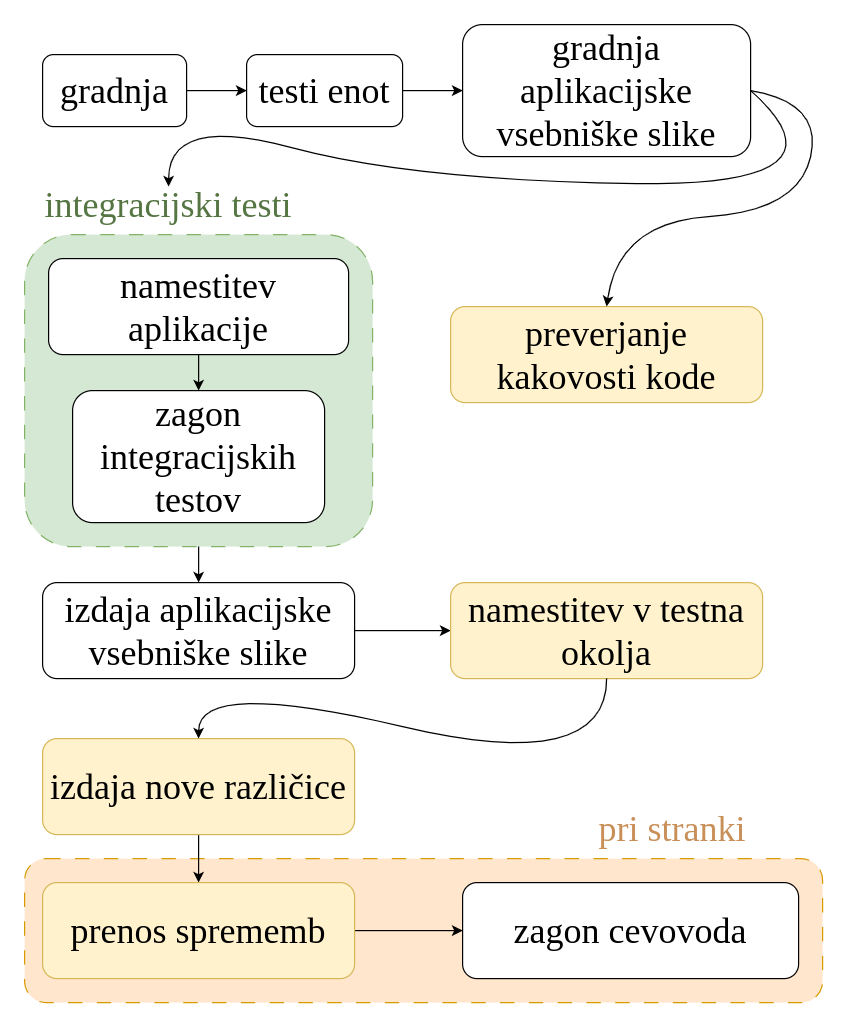
\includegraphics[width=13.5cm]{figures/osnoven-cevovod.png}
    \end{center}
\caption{Potek osnovnega cevovoda.}
\label{fig:osnoven-cevovod}
\end{figure}

Temu sledi gradnja aplikacijske vsebniške slike in njen odriv v register vsebniških slik. Zgrajeno sliko nato uporabimo za namestitev aplikacije na gručo platforme Kubernetes, ki je namenjena izvajanju integracijskih testov. Na tem mestu lahko ročno zaženemo tudi orodja za preverjanje kakovosti in varnosti kode. V kolikor so bili vsi predhodni koraki do sedaj uspešni, se aplikacijska vsebniška slika označi z ustrezno številko različice. Nato se ustvarijo naloge za namestitev aplikacije v različna testna okolja, ki omogočajo razvijalcem in zaposlenim, ki skrbijo za zagotavljanje kakovosti, da aplikacijo tudi sami preizkusijo in pogledajo. Čisto na koncu cevovoda pa so na voljo tudi naloge za izdajanje novih verzij, ki jih razvijalci lahko ročno zaženejo. Potek osnovnega cevovoda je prikazan na sliki \ref{fig:osnoven-cevovod}.

\subsection{Proces v podjetju}
\label{subsec:proces-v-podjetju}
Vodja projekta ali glavni razvijalec pripravi arhitekturo in organizacijo projekta, ki je lahko polirepo ali monorepo. Razvoj aplikacije v podjetju največkrat poteka po nalogah, ki jih vodja projekta dodeli razvijalcem v spletni platformi GitLab. Ta omogoča, da te naloge ustvarimo, opišemo njihov cilj, jim dodelimo prioritetno stopnjo, jih komentiramo, jim dodelimo zadolženega razvijalca in drugo. Implementacija naloge poteka v naslednjih korakih:
\begin{enumerate}
    \item Razvijalec prebere opis naloge in doda morebitna vprašanja glede razvoja naloge.
    \item Ko se vprašanja razrešijo, ustvari v repozitoriju novo vejo, na kateri bo razvil nalogo.
    \item Razvijalec razvija novo funkcionalnost ali popravke in sproti dodaja spremembe na svojo vejo v oddaljenem repozitoriju.
    \item Ob vsakem odrivu aplikacijske kode se izvede cevovod, ki preveri oddano kodo in razvijalca obvesti o morebitnih težavah.
    \item Ko razvijalec konča z razvojem naloge, ustvari zahtevek za združitev v glavno vejo v spletni platformi GitLab in nanj dodeli pregledovalca.
    \item Pregledovalec preveri dodane spremembe in odobri zahtevek ali pa ga zavrne ter v komentarjih pojasni, kaj je potrebno popraviti.
    \item Ko so vsi komentarji v zahtevku za združitev razrešeni, razvijalec zahtevek dodeli nekomu v projektu, ki ima pravice za združitev kode v glavno vejo.
    \item Razvijalec, ki ima pravice za združitev kode v glavno vejo, ob primernem času združi kodo v glavno vejo.
    \item Naloga se po združitvi označi za končano in bo na voljo v naslednji verziji aplikacije.
\end{enumerate}

\subsection{Proces pri naročniku}
\label{subsec:proces-pri-naročniku}
V poglavju \ref{subsec:dostava-izvorne-kode} smo opisali, zakaj je dostava izvorne kode naročniku koristna tako za naročnika kot tudi za podjetje. Da bi bil naročnik čim bolj neodvisen od podjetja, izvedemo enak cevovod z manjšimi prilagoditvami tudi na primerku spletne platforme GitLab pri naročniku. Ob izdaji nove verzije se zgodi naslednje:
\begin{itemize}
    \item Vse spremembe v repozitoriju od zadnje izdane verzije stisnemo (ang. squash) v eno spremembo in jo dodamo na posebno vejo imenovano \texttt{release}, namenjeno upravljanju različic.
    \item Vsem odgovornim v podjetju preko elektronske pošte avtomatsko sporočimo, da smo izdali novo različico.
    \item Naročnik zažene posebno nalogo, ki je del naročnikovega cevovoda in prenese spremembe v svoj repozitorij.
    \item Ko se sprememba prenese, se zažene enak cevovod kot v podjetju z nalogami za namestitev v naročnikova testna in produkcijska okolja.
\end{itemize}
Na ta način smo naročniku omogočili, da lahko sama enostavno namesti aplikacijo v svoja okolja in je zato manj odvisna od podjetja, ki je aplikacijo razvilo. V kolikor naročnik ne uporablja spletne platforme GitLab za upravljanje in nadzor različic aplikacij, pa se dogovorimo za drugačen način prevzema sprememb in namestitve aplikacij v okolja naročnika.

\section{Razvoj komponente Medius CD}
\label{sec:razvoj-komponente-medius-cd}
Komponenta za vzpostavitev cevovoda neprekinjene integracije in dostave - Medius CD je nastala z željo po poenotenju cevovodov na projektih, zmanjšanju količine podvojene konfiguracije in kode ter lažjemu vzdrževanju. Sestavljen je iz dveh delov: predlog GitLab in skript napisanih v jeziku Bash, ki omogoča lažjo integracijo z različnimi operacijskimi sistemi vsebnikov, ki jih uporabljajo izvajalci nalog GitLab.

Kot omenjeno v poglavju \ref{subsec:orodje-gitlab-ci-cd} je cevovod definiran z datoteko \texttt{.gitlab-ci.yml}, ki se nahaja na korenu projekta. Če ta datoteka obstaja v oddaljenem repozitoriju, jo GitLab avtomatsko prepozna in ob vsakem odrivu kode v oddaljen repozitorij kreira cevovod.

Naloge v cevovodu poganjajo izvajalci nalog GitLab, ki smo jih opisali v poglavju \ref{subsec:orodje-gitlab-ci-cd}. V konfiguraciji cevovoda pa lahko s ključno besedo \texttt{image} nastavimo tudi vsebniško sliko, v kateri izvajalec nalogo zažene. Takšne slike imenujemo izvajalne slike. Na ta način lahko v naprej pripravimo okolje, v katerem se naloge izvajajo. Izvajalne slike pa je potrebno naprej zgraditi in naložiti na register vsebniških slik, s katerega lahko izvajalci slike prenesejo.

Pred razvojem komponente smo izvajalne slike gradili in hranili v enem projektu GitLab. To nam je omogočalo, da smo isto sliko lahko večkrat uporabili v cevovodih različnih projektov. Kmalu pa smo ugotovili, da takšen način vodenja slik, zaradi specifik projektov, znatno oteži vzdrževanje, saj smo morali veliko slik prilagajati posameznim projektom. Odločili smo se, da bomo izvajalne slike hranili in gradili v vsakemu projektu posebej. Kljub temu pa smo pripravili vsebniško sliko \texttt{rocky-with-tools}, ki vsebuje operacijski sistem Rocky Linux\footnote{\url{https://rockylinux.org/}} in orodja, ki jih potrebujemo za izvajanje vseh cevovodov:
\begin{itemize}
    \item crane\footnote{\url{https://michaelsauter.github.io/crane/}} - orodje za orkestracijo vsebnikov z dodatnimi funkcionalnostmi in pametnejšim delovanjem. V razvitem cevovodu ga uporabljamo za spreminjanje oznake že zgrajene in shranjene vsebniške slike v registru slik. To znatno pohitri izvajanje cevovoda, ker vsebniške slike ne rabimo ponovno naložiti v register slik.
    \item gettext\footnote{\url{https://www.gnu.org/software/gettext/}} - knjižnica in orodje za prevajanje besedil v različne jezike. Velikokrat jo potrebujemo za uporabo drugih orodji.
    \item git\footnote{\url{https://git-scm.com/}} - vmesnik za ukazno vrstico za delo s sistemom za upravljanje različic Git.
    \item git-lfs\footnote{\url{https://git-lfs.com/}} - orodje za shranjevanje velikih datotek v repozitoriju v obliki kazalcev.
    \item jq\footnote{\url{https://jqlang.github.io/jq/}} - orodje za procesiranje podatkov zapisanih v formatu JSON.
    \item jsonnet\footnote{\url{https://jsonnet.org/}} - izvajalno okolje za programski jezik Jsonnet, ki smo ga omenili v poglavju \ref{subsec:jsonnet}.
    \item kubectl\footnote{\url{https://kubernetes.io/docs/tasks/tools/\#kubectl}} - vmesnik za ukazno vrstico za upravljanje z gručami na platformi Kubernetes.
    \item oc\footnote{\url{https://docs.openshift.com/container-platform/4.13/cli_reference}} - vmesnik za ukazno vrstico za upravljanje z gručami na platformi OpenShift.
    \item unzip - orodje za razširjanje datotek.
    \item wget\footnote{\url{https://www.gnu.org/software/wget/}} - orodje za prenos datotek preko najbolj razširjenih internetnih protokolov.
    \item which\footnote{\url{https://carlowood.github.io/which/}} - program za ukazno vrstico, ki izpiše absolutno pot do lokacije izvršljive datoteke podanega programa.
    \item xz\footnote{\url{https://github.com/tukaani-project/xz}} - knjižnica in orodja za stiskanje datotek.
    \item yq\footnote{\url{https://github.com/mikefarah/yq}} - orodje za procesiranje podatkov zapisanih v formatu YAML.
\end{itemize}
To sliko smo naložili na Dockerhub, tako da jo lahko uporabimo za osnovo katerekoli izvajalne slike.

Podobno velja tudi za nalogo \textit{Izdaja vsebniških slik}, ki pa se uporablja za vse projekte, ki gradijo aplikacijske vsebniške slike. V koraku gradnje za namene testiranja slike najprej označimo s številko SHA trenutnega sporočila. Ta naloga pa po uspešno izvedenih testih enako sliko označi s trenutno številko različice projekta. Na ta način lahko enostavno zamenjamo različico aplikacije, ki je nameščena.

Vsebniške slike so sestavljene iz opisa (metapodatkov) in binarnih zapisov posameznih vmesnih plasti. Organizacija registra sledi temu načelu in ne podvaja hrambe posameznih vmesnih plasti, zato s tovrstnim pristopom nismo povečali zasedenosti registra vsebnikov~\cite{Skourtis2019}.

Datoteke, na podlagi katerih zgradimo izvajalne slike projekta, hranimo v imeniku \texttt{runner-images}, ki se nahaja v korenskem imeniku projekta. V njih definiramo vse potrebno za izvedbo nalog cevovoda specifičnega projekta: tolmač programske kode, navidezne stroje, strežniške certifikate, orodja za gradnjo projekta, orodja za izvajanje testov ipd. Gradnjo izvajalnih slik pa smo avtomatizirali s posebnim projektnim cevovodom, ki se zažene, če pred zagonom cevovoda nastavimo spremenljivko GitLab \texttt{BUILD\_RUNNERS} na \texttt{true} ali pa sporočilo spremembe začnemo z besedilom \texttt{build-runners}. To smo naredili tako, da v datoteki \texttt{.gitlab-ci.yml} s ključnima besedama \texttt{include} in \texttt{rules} pogojno dodamo konfiguracijo glavnega cevovoda, ki se nahaja v \texttt{.gitlab/main.yml} ali pa konfiguracijo cevovoda za gradnjo izvajalnih slik, ki se nahaja v \texttt{.gitlab/build-runners.yml}.

\subsection{Datoteka \texttt{config\_file}}
\label{subsec:datoteka-config-file}

Platforma GitLab omogoča nastavljanje skupinskih in projektnih spremenljivk, ki so na voljo med izvajanjem nalog. Na ta način lahko v naloge dodamo občutljive podatke, kot so gesla in certifikati, ali pa nastavimo vrednosti, ki so potrebne za delovanje cevovoda. Ker smo želeli, da bi bil razvit cevovod uporaben za vse projekte, smo morali upoštevati različne zahteve, ki jih prinesejo različne specifike projektov. To smo večinoma reševali z dodajanjem spremenljivk GitLab, ki so spremenile izvajanje posameznih nalog. Ker je bilo takšnih spremenljivk veliko, je postalo vzdrževanje le teh močno zamudno, predvsem pa nepregledno. Zato smo razvili mehanizem za nastavljanje spremenljivk v cevovodu preko datoteke v formatu YAML, ki jo na začetku cevovoda prenesemo iz konfiguracijskega strežnika ali spremenljivke GitLab. Datoteko smo poimenovali \texttt{config\_file} in lahko vsebuje naslednje lastnosti:
\begin{itemize}
    \item \texttt{include} - spletni naslov ali ime spremenljivke GitLab, ki vsebuje obstoječo konfiguracijsko datoteko in jo trenutna datoteka razširja.
    \item \texttt{variables} - spremenljivke, ki so na voljo v vseh nalogah.
    \item \texttt{services} - seznam aplikacij, za katere želimo zgraditi vsebniške slike. Vsebujejo naslednje atribute:
    \begin{itemize}
        \item \texttt{name} - ime aplikacije.
        \item \texttt{dir} - pot do imenika v kateri se aplikacija nahaja.
        \item \texttt{variables} - spremenljivke, ki so na voljo pri gradnji aplikacijske slike in namestitvi aplikacije.
        \item \texttt{environments} - seznam okolji, v katera želimo aplikacijo namestiti. Vsebujejo naslednje atribute:
        \begin{itemize}
            \item \texttt{name} - ime okolja.
            \item \texttt{variables} - spremenljivke, ki so na voljo pri namestitvi aplikacije v to okolje.
        \end{itemize}
    \end{itemize}
    \item \texttt{it} - konfiguracija namestitve odvisnih aplikacij potrebnih za zagon integracijskih testov.
    \begin{itemize}
        \item \texttt{variables} - spremenljivke, ki so na voljo pri namestitvi aplikacije v okolje za integracijske teste.
        \item \texttt{deployments} - seznam aplikacij, ki jih želimo namestiti v okolje za integracijske teste. Vsebujejo naslednje atribute:
        \begin{itemize}
            \item \texttt{project}: pot do projekta na platformi GitLab.
            \item \texttt{branch}: veja, ki se uporabi za namestitev.
            \item \texttt{source}: datoteka, iz katere preberemo številko različice aplikacije, ki jo želimo namestiti.
            \item \texttt{property}: pot do atributa, ki ga želimo prebrati iz datoteke nastavljene v atributu \texttt{source}.
        \end{itemize}
    \end{itemize}
\end{itemize}

Primer datoteke \texttt{config\_file}:
\begin{verbatim}
include: http://config:8500/v1/kv/medius-cd/CONFIG_FILE
variables:
  VARIABLE_NAME: variable_value
services:
  - name: MY_PROJECT
    dir: ./service_dir
    variables:
      VARIABLE_NAME: variable_value
    environments:
      - name: test_1
        variables:
          VARIABLE_NAME: variable_value
      - test_2
it:
  variables:
    VARIABLE_NAME: variable_value
  deployments:
    - project: medius/ci-tools/medius-cd
      branch: dev
    - project: medius/ci-tools/medius-cd
      source: pom.xml
      property: version.medius-cd
\end{verbatim}

Osnovna enota cevovoda na platformi GitLab je naloga. Najbolj preprosta naloga je sestavljena iz imena naloge in dela \texttt{script}:

\begin{verbatim}
hello-world:
  script:
    - echo "Hello World!"    
\end{verbatim}

Nalogi pa lahko nastavimo še veliko drugih atributov, ki definirajo njeno delovanje. Najbolj pogosto uporabljeni so:
\begin{itemize}
    \item \texttt{artifacts} - Datoteke in imeniki, ki so po uspešno izvedeni nalogi na voljo za prenos. V nadaljevanju jih imenujemo artefakti.
    \item \texttt{before\_script} - Množica ukazov, ki se izvedejo preden se izvede naloga.
    \item \texttt{cache} - Seznam datotek, ki se shranijo v začasno shrambo in so na voljo med zaporednimi izvajanji cevovoda.
    \item \texttt{dependencies} - Seznam predhodnih nalog, iz katerih se prenesejo artefakti.
    \item \texttt{extends} - Seznam predhodnih konfiguracij, ki jih ta naloga deduje.
    \item \texttt{needs} - Seznam predhodnih nalog, po katerih se naloga takoj zažene, ne glede na to, v katerem koraku izvajanja se cevovod nahaja.
    \item \texttt{rules} - Seznam pogojev, ki določijo ali se naloga kreira ali ne.
    \item \texttt{script} - Lupinski skript, ki ga naloga izvede.
    \item \texttt{stage} - Korak cevovoda, v katerem se bo naloga izvedla.
    \item \texttt{variables} - Spremenljivke, ki so na voljo v nalogi.
    \item \texttt{when} - Kdaj se naloga zažene.
\end{itemize}

V delu \texttt{script} lahko uporabimo jezik Bash, s katerim definiramo kaj naloga naredi. Tak način definicije nalog je dober za preproste naloge, ki ne potrebujejo kompleksne logike. Za definicijo bolj kompleksnih nalog pa se boljše izkažejo skripti, ki jih napišemo v ločeni datoteki in jih v okviru naloge zaženemo. Na ta način lahko skripte tudi testiramo in uporabimo na več mestih. Zato smo logiko bolj kompleksnih nalog definirali v samostojnih skriptah, napisanih v jeziku Bash. V okviru cevovoda projekta Medius CD jih zapakiramo v različne formate, ki jih naložimo na centralni repozitorij Nexus, od koder jih lahko enostavno prenesemo in uporabljamo.

Ker se projekti lahko močno razlikujejo tako vsebinsko kot tudi tehnično - programski jezik, orodja za gradnjo, orodja za zagon testov - smo pripravili več manjših predlog GitLab, ki jih lahko večkrat uporabimo, da kreiramo različne cevovode. Pripravljene predloge se nahajajo v repozitoriju komponente Medius CD in jih lahko dodamo v predloge ostalih projektov s ključno besedo \texttt{include}. Ta nam omogoča dodajanje predlog na tri načine:
\begin{itemize}
    \item podamo pot do datoteke v lokalnem imeniku,
    \item navedemo spletni naslov do datoteke,
    \item kombinacija projekta GitLab, reference v obliki veje ali označbe Git v oddaljenem repozitoriju in poti do datoteke v oddaljenem projektu. Primer: \begin{verbatim}
include:
  - project: 'medius/ci-tools/medius-cd'
    ref: v2.3.5
    file:
      - '/gitlab-ci/templates/generic/.build.docker.yml'
\end{verbatim}
\end{itemize}
V nadaljevanju opišemo posamezne naloge, ki so del večine cevovodov.


\subsection{Inicializacija komponente Medius CD}
Prva naloga vseh cevovodov je inicializacija komponente Medius CD. Naloga poskusi najprej prebrati datoteko \texttt{config\_file.yaml} iz konfiguracijskega strežnika ali spremenljivke GitLab. V kolikor datoteka obstaja, pripravi dve novi datoteki, ki sta dodani kot artefakta:
\begin{itemize}
    \item \texttt{config\_file.json} - pretvorjen \texttt{config\_file.yaml} iz formata YAML v format JSON z nekaterimi dodanimi privzetimi spremenljivkami, če še niso bile dodane v \texttt{config\_file.yaml}.
    \item \texttt{config.env} - datoteka, ki ima v vsaki vrstici po eno spremenljivko in njeno vrednost, ločeno z enačajem. To so tiste spremenljivke, ki morajo biti na voljo v vseh nalogah. To datoteko nastavimo kot poseben artefakt pod atribut \texttt{artifacts.reports.dotenv}, kar povzorči, da se na začetku vsake naloge, ki je odvisna od te naloge, vse spremenljivke v tej datoteki nastavijo kot okoljske spremenljivke.
\end{itemize}

Naloga nato poskusi prebrati številko različice komponente Medius CD, ki je definirana pod ključno besedo \texttt{include} v datoteki \texttt{.gitlab/.main.yml}. Številka različice se uporabi za prenos komponente iz centralnega repozitorija Nexus. Če številka različice ni definirana ali jo naloga ne zna prebrati, se prenese zadnja objavljena različica. Naloga razširi paket v imenik, ki je nastavljen s spremenljivko \texttt{MEDIUS\_CD\_PATH} in ga doda med artefakte, kjer je na voljo za ostale naloge.

\subsection{Gradnja projekta in testi enot}

Naslednji dve nalogi sta gradnja projekta in zagon testov enot. Obe nalogi sta odvisni od programskega jezika in orodij, ki jih projekt uporablja. V projektu Medius CD imamo pripravljene naloge za gradnjo in zagon testov enot projektov, ki uporabljajo:
\begin{itemize}
    \item programski jezik Java in orodje Maven,
    \item Python, orodje setuptools in orodje tox,
    \item JavaScript ali TypeScript in orodje npm ter
    \item JavaScript ali TypeScript in orodje pnpm.
\end{itemize}

\subsection{Gradnja vsebniških slik}
Po uspešni gradnji projekta in testih enot se zaženejo naloge, ki zgradijo vsebniške slike. Če je projekt sestavljen iz več aplikacijskih modulov, je potrebno zgraditi več različnih aplikacijskih vsebniških slik. To naredimo tako, da v konfiguracijski datoteki \texttt{config\_file} pod ključno besedo \texttt{services} definiramo več servisov. Prva naloga v koraku gradnje slik na podlagi konfiguracijske datoteke in z uporabo orodja \texttt{jsonnet} pripravi konfiguracijsko datoteko GitLab v formatu JSON, ki vsebuje naloge za gradnjo vseh aplikacijskih slik, definiranih v konfiguracijski datoteki \texttt{config\_file}. Ta datoteka se nato uporabi v nalogi tipa \texttt{trigger}, ki na podlagi prejete datoteke kreira nov podrejen cevovod (ang. child pipeline). Ta cevovod vsebuje naloge, ki zaženejo skript napisan v programskem jeziku Bash, ki na podlagi datoteke, ki deklarira vsebniško sliko, in z uporabo orodja \texttt{kaniko} zgradi sliko, jo naloži v projektni register vsebniških slik ter jo označi s številko SHA trenutnega sporočila. Tako je slika pripravljena za zagon integracijskih testov ali namestitev na testna okolja.

\subsection{Preverjanje kakovosti kode}
Vzporedno z gradnjo vsebniških slik lahko ročno zaženemo nalogo za preverjanje kakovosti kode. Ta je ponovno odvisna od programskega jezika in orodij, ki jih projekt uporablja. V nalogi se zažene orodje platforme SonarQube, ki smo ga opisali v poglavju \ref{sec:sonarqube}, ki preveri ali koda vsebuje primere slabih praks in znane varnostne pomanjkljivosti ter rezultate naloži na platformo SonarQube in se zapiše v datoteke, ki so na voljo med artefakti.

% trigger -> nov pipeline -> trigger, ki kreira nov pipeline s deploy it in trigger na druge projekte
\subsection{Integracijski testi}
Po uspešni gradnji vsebniških slik lahko ročno zaženemo nalogo za zagon integracijskih testov. Zaradi daljšega trajanja jih ne želimo avtomatsko zagnati v vseh cevovodih. Za testiranje integracije potrebujemo:
\begin{itemize}
    \item testno bazo, če aplikacija za delovanje potrebuje bazo,
    \item nameščeno aplikacijo,
    \item nameščene aplikacije, na katere se razvita aplikacija integrira.
\end{itemize}
Zato je naloga za zagon integracijskih testov tipa \texttt{trigger} in kreira podrejen cevovod. Cevovod je definiran kar z enako konfiguracijsko datoteko GitLab, ki jo uporablja cevovod aplikacije, vendar ima nastavljeno spremenljivko GitLab \texttt{IT\_FORCE} na \texttt{true}. To povzroči, da podrejen cevovod vsebuje naslednje naloge:
\begin{itemize}
    \item \texttt{initialize-database} - Na podlagi datotek, ki so dodane v repozitorij, pripravi testno bazo.
    \item \texttt{initialize-it-runtime} - Iz konfiguracijske datoteke \texttt{config\_file} pripravi datoteko v formatu \texttt{properties}, ki vsebuje spremenljivke za zagon integracijskih testov - spletni naslov aplikacije, naslov baze ipd.
    \item \texttt{prepare-deploy-it} - Naloga tipa \texttt{trigger}, ki na podlagi konfiguracije pod ključno besedo \texttt{it} v konfiguracijski datoteki \texttt{config\_file}, kreira podrejen cevovod z nalogami, ki namestijo vse odvisne aplikacije. Naloge za namestitve drugih aplikacij, so zopet tipa \texttt{trigger}, saj zaženejo cevovod druge aplikacije s tako nastavljenimi spremenljivkami, da se namestijo v enako okolje kot testirana aplikacija.
    \item \texttt{test} - Po uspešni namestitvi aplikacij s pomočjo orodja za testiranje zažene integracijske teste
    \item \texttt{clean-up-database} - Po končanem izvajanju testov izbriše testno bazo.
    \item \texttt{clean-up-namespace} - Po končanem izvajanju testov izbriše testno okolje na gruči platforme Kubernetes.
\end{itemize}

\subsection{Izdaja paketov in vsebniških slik}
Nekatere naloge želimo izvesti samo na določenih vejah repozitorija. To lahko naredimo s ključnima besedama \texttt{rules} in \texttt{if} s katerima določimo logični pogoj, ki definira, kdaj naj se naloga doda v cevovod. Takšni nalogi sta tudi \textit{Izdaja paketov} in \textit{Izdaja vsebniških slik}, ki ju dodamo v cevovod samo ob spremembah na vejah imenovanih \texttt{dev} ali \texttt{main} in novih značkah.

Izdaja paketov je del cevovoda projektov, ki se uporabljajo kot knjižnice v drugih projektih. Naloga zapakira kodo v paket in ga naloži na centralni repozitorij Nexus, od koder ga lahko ostali projekti prenesejo in uporabijo. Na ta način se na centralnem repozitoriju vedno nahajajo vse verzije kot tudi trenutna razvojna verzija projekta, ki se nahaja v veji \texttt{dev} ali \texttt{main}.

Podobno velja tudi za nalogo \textit{Izdaja vsebniških slik}, ki pa se uporablja za vse projekte, ki gradijo aplikacijske vsebniške slike. V koraku gradnje za namene testiranja slike najprej označimo s številko SHA trenutnega sporočila. Ta naloga pa po uspešno izvedenih testih enako sliko označi s trenutno številko različice projekta. Na ta način lahko enostavno zamenjamo različico aplikacije, ki je nameščena.

\subsection{Namestitev aplikacije}
\label{subsec:namestitev-aplikacije}
Naloge za namestitev aplikacije v različna okolja se podobno kot pri gradnji vsebniških slik in integracijskih testih dodajo dinamično s pomočjo naloge tipa \texttt{trigger}. Ta naloga prebere konfiguracijo okolij, ki je za vsak servis posebej definirana v konfiguracijski datoteki \texttt{config\_file} in kreira nove naloge za namestitev aplikacije v različna okolja. Ustvarjene naloge najprej zaženejo skript \texttt{init-kube-openshift.sh}, ki pripravi konfiguracijsko datoteko za povezavo na gručo platforme Kubernetes, nato pa še skript \texttt{job-deploy.sh}, ki naredi naslednje:
\begin{itemize}
    \item Prebere datoteko \texttt{/deploy/k8s/deployment.yml.in}, ki se nahaja v repozitoriju in predstavlja predlogo namestitve.
    \item V prebrani datoteki poišče vse besede, ki se začnejo in končajo z dvemi podčrtaji npr. \texttt{\_\_SERVICE\_NAME\_\_}. Te besede predstavljajo spremenljivke, ki jih je potrebno zamenjati z vrednostmi.
    \item Vse spremenljivke v datoteki zamenja z vrednostmi, ki jih imajo okoljske spremenljivke z enakim imenom, vendar brez podčrtajev, kot je na primer \texttt{SERVICE\_NAME}, in ustvari novo konfiguracijsko datoteko za namestitev na gručo platforme Kubernetes imenovano \texttt{deployment.yml}.
    \item S programom \texttt{kubectl} in ustvarjeno datoteko kreira novo namestitev na gruči platforme Kubernetes.
    \item S programom \texttt{kubectl} preverja stanje namestitve dokler aplikacija ni uspešno nameščena ali pa preteče 10 minut, ko se naloga neuspešno zaključi.
\end{itemize}

\subsection{Izdaja nove različice}
Nova različica se izdaja periodično ali pa ob posamezni zaključeni enoti, zato je nalogo za izdajo nove različice potrebno ročno zagnati. Naloga pa zažene skripto \texttt{job-release-src-to-branch.sh}, ki avtomatizira izdajo izdelane kode naročniku. Skripta izvede naslednje korake:
\begin{itemize}
    \item Stisne vse spremembe od zadnje izdane verzije v eno spremembo.
    \item Datoteki \texttt{.gitlab/main.yml} in \texttt{.gitlab/build-runners.yml}, oziroma datoteke, ki so nastavljene s spremenljivko \texttt{GITLAB\_CI\_PATH}, posodobi z uporabo končne točke programskega vmesnika GitLab, ki vse dodane predloge preko ključne besede \texttt{include} in ostalo vsebino združi v eno datoteko. Na ta način lahko naročnik zažene cevovod tudi v svoji instanci platforme GitLab, ki nima dostopa do predlog, ki se nahajajo v projektu Medius CD.
    \item Iz številke različice aplikacije odstrani \texttt{-SNAPSHOT} oziroma \texttt{-rc}.
    \item Doda številko različice v datoteko \texttt{CHANGELOG.md}, ki vsebuje povzetek sprememb, ki so bile narejene v tej verziji.
    \item Vse našteto doda kot eno spremembo v vejo \texttt{release}.
\end{itemize}
Na ta način se v veji \texttt{release} za vsako različico nahaja po ena sprememba, kar omogoča, da si lahko naročnik spremembe enostavno prenese v svoj repozitorij.

Na koncu naloga zažene še skripta \texttt{gitlab-create-tag-with-notes.sh}, ki ustvari novo značko Git s pripono \texttt{-SNAPSHOT} ali \texttt{-rc}, in \texttt{bump-version.sh}, ki poveča trenutno številko različice v razvoju, npr. iz \texttt{0.3.0-SNAPSHOT} v \texttt{0.4.0-SNAPSHOT} ter doda spremembo v vejo, na kateri je bil cevovod pognan.

\subsection{Prilagajanje nalog}
\label{subsec:prilagajanje-nalog}
V kolikor vnaprej pripravljene predloge cevovodov ne zadoščajo potrebam projekta, lahko vzdrževalec projekta z uporabo predlog posameznih nalog kreira cevovod po meri. Predloge nalog so narejene tako, da ne uporabljajo ključne besede \texttt{before\_script}. To omogoča, da lahko naloge v končnem projektu dodamo preko ključne besede \texttt{include}, nato pa jih prilagodimo z dodajanjem skript v delu \texttt{before\_script}. Obenem je možno naloge konfigurirati tudi s prepisom dela naloge, ki ga želimo prilagoditi, in nastavljanjem spremenljivk, ki so opisane v dokumentaciji komponente.

% \section{Dokumentacija}
% Dokumentacija projekta \texttt{medius-cd} je narejena z uporabo orodja \texttt{sphinx} in funkcionalnosti \texttt{gitlab-pages} platforme GitLab.

\section{Vtičnik GitLab Template Lint}
\label{sec:vtičnik-gitlab-template-lint}
Med razvojem predlog konfiguracijskih datotek orodja GitLab CI/CD smo s ključno besedo \texttt{include} zmanjšali podvojenost konfiguracije in kode. S tem pa smo zmanjšali preglednost konfiguracije in otežili razhroščevanje in preverjanje pravilnosti predlog. Predloge smo zato preverjali z orodjem platforme GitLab, ali pa z odrivom spremembe na ločeno vejo v repozitoriju in preverjanjem statusa novo nastalega cevovoda. Oba načina sta zelo časovno potratna in okorna, saj je med razvojem potrebno zapustiti integrirano okolje. Zato smo se odločili, da razvijemo vtičnik za integrirano okolje IntelliJ IDEA, s katerim dodamo funkcionalnost za preverjanje pravilnosti konfiguracijskih datotek GitLab in s tem znatno pohitrimo razvoj.

Razvoja vtičnika smo začeli s predlogo za razvoj vtičnika platforme IntelliJ IDEA\footnote{\url{https://github.com/JetBrains/intellij-platform-plugin-template}}, ki je javno dostopna na platformi GitHub in uporablja programski jezik Kotlin ter za gradnjo orodje Gradle. Predloga vsebuje vnaprej pripravljeno:
\begin{itemize}
    \item strukturo projekta,
    \item dodane odvisnosti, ki jih za razvoj vtičnika potrebujemo,
    \item konfiguracijsko datoteko za cevovod CI na platformi GitHub
\end{itemize}

\subsection{Ideja vtičnika}
\label{sec:vtičnik-gitlab-template-lint-ideja}
Platforma GitLab za integracijo z drugimi aplikacijami izpostavlja programski vmesnik z arhitekturnim stilom REST. Izpostavlja tudi končno točko za preverjanje konfiguracijskih datotek platforme GitLab. Ideja vtičnika je preprosta, saj izvede zgolj en klic na programski vmesnik: 
\begin{enumerate}
    \item Uporabnik v integriranem razvojnem okolju spremeni konfiguracijsko datoteko,
    \item vtičnik zazna spremembo in pošlje zahtevek z žetonom za avtentikacijo na končno točko za preverjanje konfiguracijskih datotek,
    \item vtičnik iz odgovora programskega vmesnika prebere ali je konfiguracija pravilna in v primeru napake v integriranem okolju prikaže opozorilo.
\end{enumerate}

\begin{figure}
    \begin{center}
        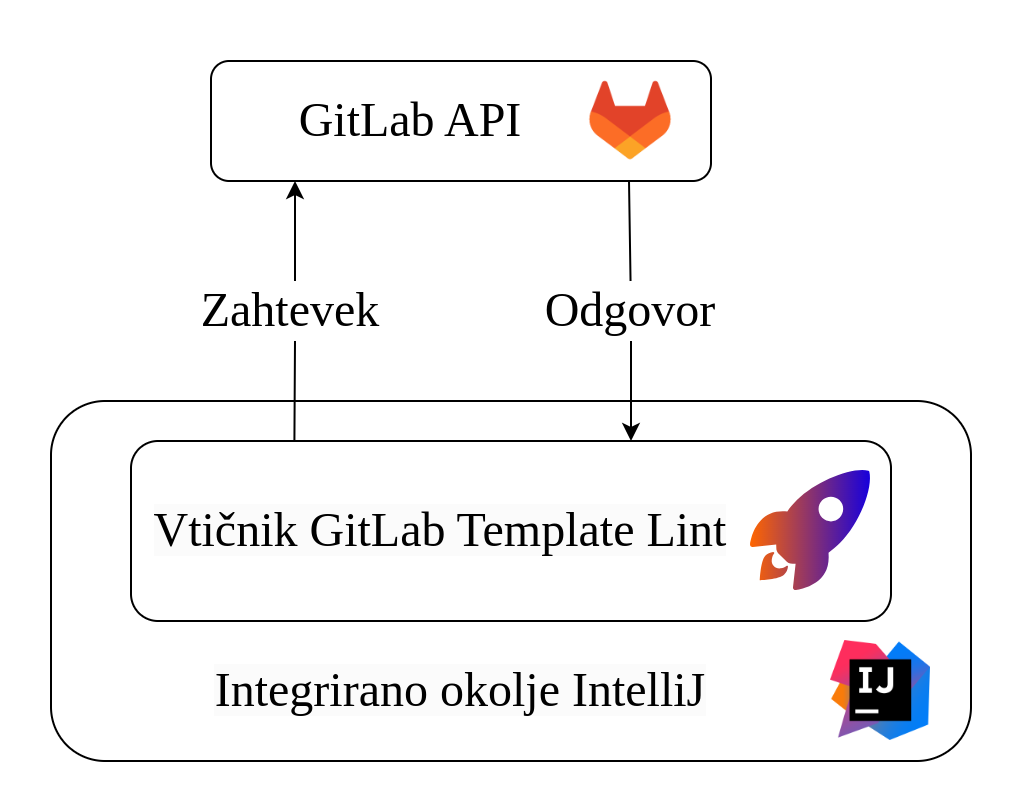
\includegraphics[width=9cm]{figures/gitlab-template-lint-ideja.png}
    \end{center}
\caption{Vizualizacija ideje vtičnika.}
\label{fig:vizualizacija-gitlab-template-lint}
\end{figure}

Preproste ideje pa ni bilo tako enostavno razviti, saj smo pri izdelavi naleteli še na nekaj izzivov. V naslednjih podpoglavjih opišemo kakšne težave smo imeli in kako smo jih rešili.

\subsection{Nastavitve vtičnika}
\label{sec:vtičnik-gitlab-template-lint-nastavitve}
Programski vmesnik platforme GitLab za avtentikacijo zahtevkov omogoča več načinov. V našem primeru se je za najbolj preprost in praktičen način izkazala avtentikacija z žetonom, ki ga uporabniki vtičnika lahko pridobijo na platformi GitLab in vnesejo v nastavitve vtičnika.

Integrirano orodje IntelliJ IDEA za razvoj uporabniških vmesnikov vtičnikov nudi domensko specifičen jezik (ang. Domain-Specific Language - DSL) imenovan Kotlin UI, ki omogoča razvoj uporabniških vmesnikov v programskem jeziku Kotlin. Slednje smo uporabili tudi sami, da smo oblikovali uporabniški vmesnik za nastavitve našega vtičnika, ki ga lahko vidimo na sliki \ref{fig:gitlab-template-lint-nastavitve}. Glavni nastavitvi vtičnika sta:
\begin{itemize}
    \item pogostost preverjanja (ang. lint frequency) - kako pogosto se pošlje zahtevek na programski vmesnik platforme GitLab. Možnosti so: 
    \begin{itemize}
        \item ob vsaki spremembi v datoteki,
        \item po shranjevanju datoteke,
        \item ko uporabnik ročno zažene akcijo za preverjanje. 
    \end{itemize}
    Na ta način omogočimo uporabnikom, da zmanjšajo število zahtevkov na programski vmesnik platforme GitLab in na ta način zmanjšajo obremenjenost platforme.
    \item žeton za avtentikacijo s platformo GitLab (ang. Gitlab API token) - urejanje žetona za posamezen spletni naslov platforme GitLab je omogočeno preko tabele, v katero lahko uporabniki vnesejo več različnih žetonov za različne instance platforme GitLab. S tem omogočimo, da imajo uporabniki lahko v razvojnem okolju odprtih več projektov, katerih oddaljeni repozitoriji se nahajajo na različnih instancah platforme GitLab.
\end{itemize}

\begin{figure}
    \begin{center}
        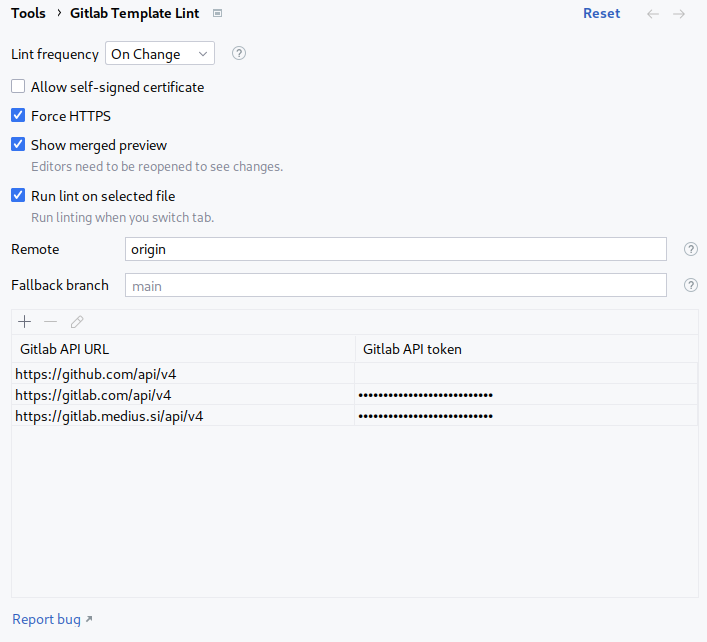
\includegraphics[width=13.5cm]{figures/gitlab-template-lint-nastavitve-1.png}
    \end{center}
\caption{Nastavitve vtičnika.}
\label{fig:gitlab-template-lint-nastavitve}
\end{figure}

\subsection{Preverjanje konfiguracijskih datotek}
\label{sec:vtičnik-gitlab-template-lint-razvoj}
Preverjanje konfiguracijskih datotek smo razvili v obliki cevovoda, ki vsebuje naslednje korake:
\begin{enumerate}
    \item Razreševanje konteksta - glede na to, katera datoteka je trenutno odprta v urejevalniku, poskusimo ugotoviti spletni naslov repozitorija in spletni naslov do programskega vmesnika GitLab instance, v kateri se repozitorij nahaja.
    \item Razreševanje žetona za avtentikacijo - iz nastavitev vtičnika poskusimo prebrati žeton za avtentikacijo s programskim vmesnikom GitLab, ki je nastavljen za spletni naslov programskega vmesnika, ki smo ga razrešili v prejšnjem koraku.
    \item Razreševanje identifikacijske številke projekta - s spletnim naslovom repozitorija, ki smo ga pridobili v prvem koraku, in žetonom, ki smo ga pridobili v drugem koraku, naredimo poizvedbo na programski vmesnik platforme GitLab, da pridobimo identifikacijsko številko projekta.
    \item Preverjanje konfiguracijske datoteke - vsebino trenutno odprte datoteke skupaj z žetonom pošljemo na končno točko za preverjanje konfiguracijskih datotek orodja GitLab CI/CD, preberemo odgovor in v primeru napake v trenutno odprtem urejevalniku prikažemo napako.
\end{enumerate}

\subsection{Prikaz združene konfiguracije}
Kot omenjeno v poglavju \ref{sec:razvoj-komponente-medius-cd}, lahko v konfiguracijskih datotekah s ključno besedo \texttt{include} v konfiguracijsko datoteko dodajamo obstoječe predloge, s ključno besedo \texttt{extend} pa lahko posamezne naloge razširjamo z že obstoječimi nalogami. To je zelo uporabno za zmanjšanje podvojenosti konfiguracije, vendar pa lahko oteži razhroščevanje v primeru napak, ker v konfiguracijski datoteki ne vidimo celotne vsebine, ki jo orodje GitLab CI/CD uporabi za kreiranje cevovoda.

Zato smo kmalu po razviti funkcionalnosti za preverjanje konfiguracije v vtičnik dodali še funkcionalnost za prikazovanje vsebine združene konfiguracije. To je bilo dokaj preprosto, saj v odgovoru na zahtevek za preverjanje konfiguracijske datoteke dobimo tudi vsebino združene konfiguracijske datoteke. Pregled združene konfiguracijske datoteke smo dodali tako, da smo razširili obstoječi urejevalnik kode, ki se uporablja za urejanje konfiguracijskih datotek, s predogledom združene konfiguracijske datoteke na desni strani urejevalnika. Delovanje vtičnika je prikazano na sliki \ref{fig:gitlab-template-lint-primer-1}.

\begin{figure}
    \begin{center}
        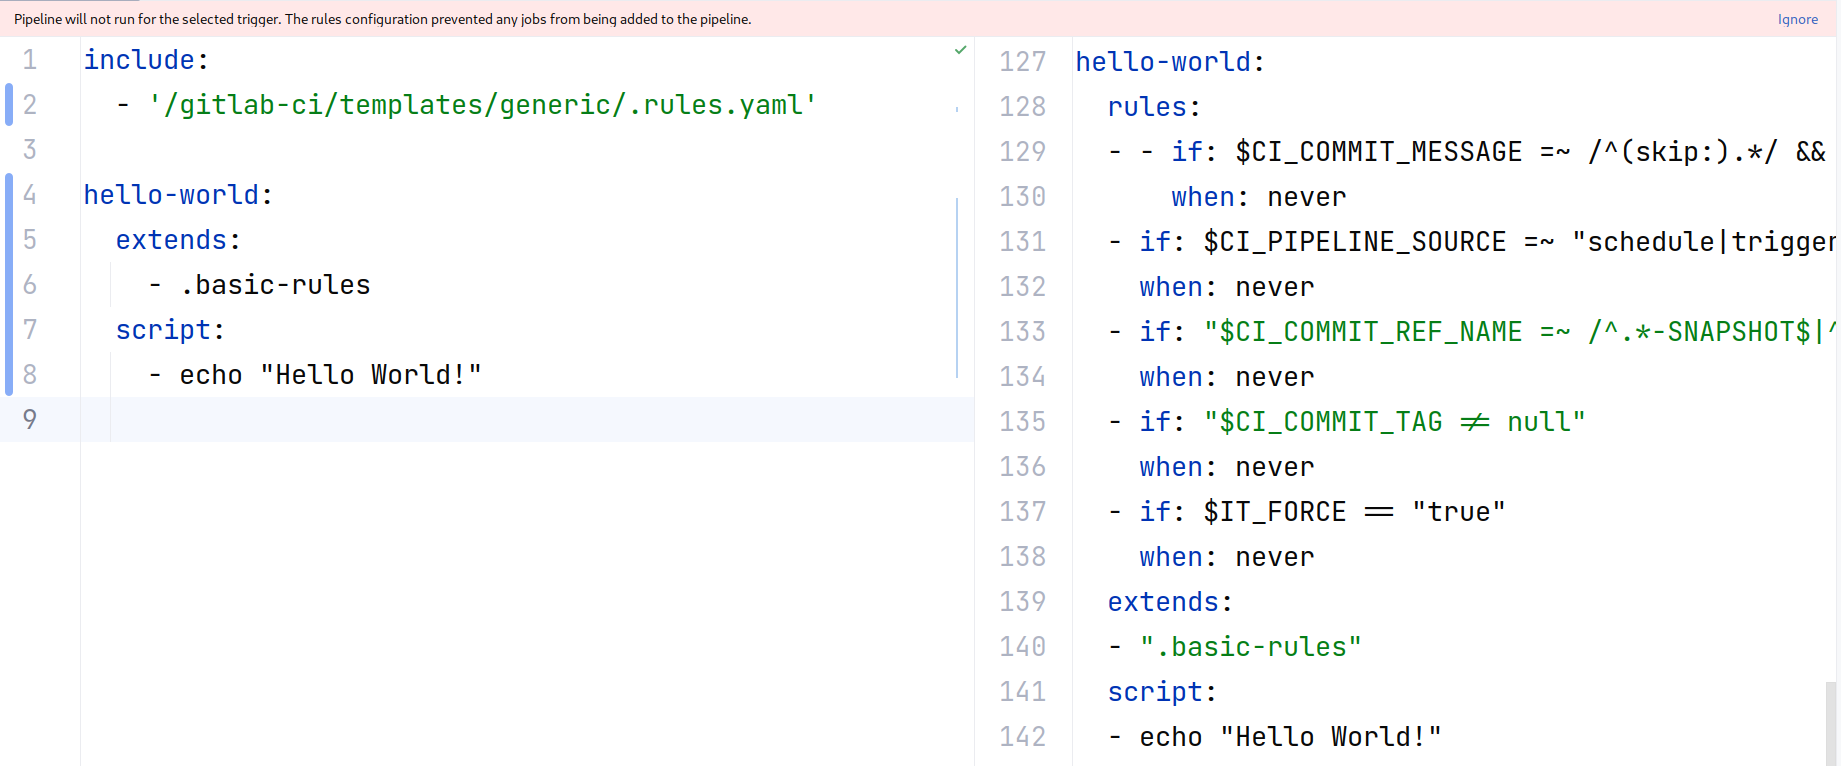
\includegraphics[width=13.5cm]{figures/gitlab-template-lint-primer-1.png}
    \end{center}
\caption{Primer delovanja vtičnika.}
\label{fig:gitlab-template-lint-primer-1}
\end{figure}

%----------------------------------------------------------------
% Poglavje 5 - Rezultati
%----------------------------------------------------------------


\chapter{Rezultati}
\label{ch:rezultati}
V tem poglavju bomo razpravljali o ključnih rezultatih doseženih v okviru naše magistrske naloge. Najprej se bomo osredotočili na izboljšanje priprave izvajalnih slik, ki igrajo ključno vlogo pri izvajanju cevovoda projekta. Nato bomo opisali še eno pomembno prednost uporabe konfiguracijske datoteke \texttt{config\_file} in pokazali, kako enostavno lahko z uporabo razvite komponente vzpostavimo cevovod za razvoj aplikacije in programske knjižnice. Poleg tega bomo predstavili praktične primere uporabe te komponente na treh resničnih projektih, ki se trenutno razvijajo ali pa so že v fazi produkcije. Ti projekti uporabljajo različne programske jezike in imajo raznolike zahteve, kar nam omogoča, da pokažemo univerzalnost naše rešitve. Na koncu bomo ocenili uspeh vtičnika Gitlab Template Lint in razpravljali o njegovih prednostih in izpostavili tudi njegove omejitve.

\section{Gradnja izvajalnih slik}
\label{sec:gradnja-izvajalnih-slik}
V poglavju \ref{sec:razvoj-komponente-medius-cd} smo opisali, kako zgradimo izvajalne slike, ki jih uporabljajo izvajalci nalog GitLab ali pa jih potrebujemo za gradnjo aplikacijskih vsebniških slik. Omenili smo tudi, da smo pred razvojem komponente Medius CD te slike gradili in hranili v enem projektu, kar je otežilo njihovo vzdrževanje. Večino končnih izvajalnih slik je bilo zgrajenih na osnovi starševskih slik, ki so imele odvisnosti tudi na svoje starševske slike in tako dalje. Tako se je cevovod zelo razvejal, kar lahko vidimo tudi na sliki \ref{fig:gradnja-izvajalnih-slik-pred}. V primeru, da se je spremenila osnovna slika v korenu hierarhije, je bilo potrebno skoraj vse slike ponovno zgraditi, kar je lahko trajalo tudi več kot 30 minut.

\begin{figure}
    \begin{center}
        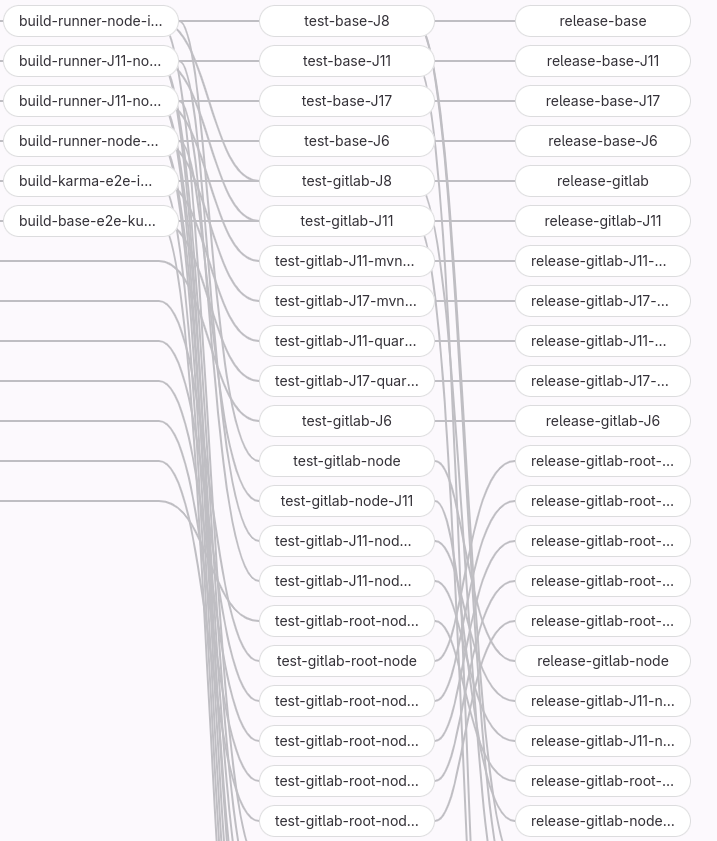
\includegraphics[width=13cm]{figures/gradnja-izvajalnih-slik-2.png}
    \end{center}
\caption{Cevovod za gradnjo izvajalnih slik pred razvojem komponente Medius CD.}
\label{fig:gradnja-izvajalnih-slik-pred}
\end{figure}

V razviti komponenti smo uvedli poseben cevovod za gradnjo izvajalnih slik, ki je del vsakega projekta in ga lahko ročno zaženemo. To nam zelo olajša vzdrževanje izvajalnih slik, saj cevovod vsebuje samo naloge za gradnjo slik, ki jih posamezen projekt potrebuje. Tako cevovod ostane obvladljiv in se tudi hitreje izvede. Obenem zgrajeno sliko hranimo v registru projekta in jo uporabljamo samo za projekt, v katerem je bila zgrajena. To omogoča fleksibilnost, da lahko sliko čim bolj prilagodimo potrebam projekta. Rešimo tudi problem starševstva tako, da zmanjšamo število staršev z uporabo slike \texttt{rocky-with-tools}, ki smo jo omenili v poglavju \ref{sec:razvoj-komponente-medius-cd} in vsebuje vsa potrebna orodja za izvajanje cevovoda. To sliko uporabimo kot starševsko sliko v vseh zagonskih in aplikacijskih slikah. Za varnostne posodobitve pa poskrbimo z rednimi avtomatskimi zagoni cevovoda za gradnjo vsebniških slik.


\section{Prilagajanje cevovoda}
V poglavju \ref{subsec:datoteka-config-file} smo predstavili datoteko \texttt{config\_file}, ki nam omogoča konfiguracijo cevovoda z datoteko v formatu YAML. Poleg olajšanja vzdrževanja vseh spremenljivk, ki so potrebne za prilagoditev cevovoda projektnim specifikam, nam ta datoteka olajša tudi prilagajanje cevovoda naročniku. Naročnik največkrat uporablja svoj centralni repozitorij, konfiguracijski strežnik, register vsebniških slik in drugo. Hkrati se namestitvena okolja v podjetju in pri naročniku razlikujejo. Konfiguracijska datoteka omogoča, da lahko naročnik sam enostavno spremeni nastavitve svojega cevovoda. To znatno olajša razvoj aplikacije, saj konfiguracija cevovoda ni dodana v sistem za nadzor različic in za spremembo obnašanja cevovoda ni potrebno izdajati nove različice aplikacije.

\section{Cevovod aplikacije}
\label{sec:projekt-aplikacije}
Z novo razvito komponento je cevovod za razvoj aplikacije enostavno dodati. V korenski imenik projekta dodamo naslednje imenike in datoteke:
\begin{itemize}
    \item Imenik \texttt{runner-images} v katerega dodamo datoteke, ki definirajo vsebniške slike in vsebujejo ukaze za namestitev orodij, ki jih potrebujemo za gradnjo aplikacije ali aplikacijske vsebniške slike. Za osnovno lahko uporabimo pripravljeno sliko \texttt{rocky-with-tools}, ki že vsebuje vsa osnovna orodja, potrebna za izvajanje nalog.
    \item Imenik \texttt{deploy/docker} v katerega dodamo datoteko, ki definira aplikacijsko vsebniško sliko in vsebuje ukaze za namestitev in zagon aplikacije v vsebniku.
    \item Imenik \texttt{deploy/k8s} v katerega dodamo predlogo \texttt{deployment.yml.in}, ki vsebuje konfiguracijo za namestitev na gručo na platformi Kubernetes.
    \item Vnaprej pripravljeno datoteko \texttt{.gitlab-ci.yml}, ki pogojno doda konfiguracijski datoteki za cevovod za gradnjo izvajalnih slik ali aplikacijski cevovod.
    \item Imenik \texttt{.gitlab}, v katerega dodamo datoteki \texttt{.build-runners.yml}, ki uporabi predlogo za gradnjo izvajalnih slik, in \texttt{.main.yml}, ki uporabi predlogo aplikacijskega cevovoda.
\end{itemize}

\section{Cevovod programske knjižnice}
Za postavitev cevovoda projekta, ki vsebuje programsko knjižnico potrebujemo enake imenike in datoteke, z izjemo imenika \texttt{deploy}, ki ga ne potrebujemo, saj knjižnice ne moremo namestiti na gručo platforme Kubernetes. Tudi vsebina datotek ostane v večini enaka, edina razlika je v datoteki \texttt{.main.yml}, v kateri moramo uporabiti predlogo cevovoda za programsko knjižnico. V primeru, da se za testiranje knjižnice potrebuje testno aplikacijo, ki knjižnico uporablja, se v imenik \texttt{deploy} doda konfiguracijske datoteke za namestitev testne aplikacije. Namesto namestitve, pa knjižnico na koncu cevovoda naložimo v centralni repozitorij za upravljanje različic. Na ta način jo lahko enostavno uporabimo v drugih aplikacijah.

\section{Projekt v programskem jeziku Java}
\label{sec:java-projekt}
V tem poglavju bomo predstavili postavitev cevovoda projekta, ki vsebuje aplikacijo, napisano v programskem jeziku Java in za gradnjo aplikacije uporablja orodje Maven. Aplikacija uporablja aplikacijski strežnik Wildfly\footnote{\url{https://www.wildfly.org/}} in preko programskega vmesnika izpostavlja končne točke za pridobivanje podatkov o izvedenih denarnih transakcijah podjetja, ki se prikazujejo v čelni aplikaciji. Za shranjevanje podatkov uporablja podatkovno bazo Oracle\footnote{\url{https://www.oracle.com/database/}}.

Kot smo že omenili v prejšnjih poglavjih, je razvoj poslovno kritičnih aplikacij zelo odvisen od zahtev naročnika. Zaradi zmanjšanje odvisnosti naročnika od podjetja, kot smo omenili v poglavju \ref{sec:neprekinjena-dostava}, pa želimo izvajanje cevovoda omogočiti tudi na naročnikovi instanci platforme GitLab. V primeru tega projekta, je naročnika zaradi varnosti zahteval, da se celoten cevovod izvaja brez povezave na internet. To pomeni, da morajo biti vse odvisnosti projekta dostopne preko internih repozitorijev in registrov, do katerih skripti v nalogah lahko dostopajo. To smo upoštevali tudi pri zasnovi komponente Medius CD in izdelali cevovod, ki ga lahko takšnim zahtevam prilagodimo.

\subsection{Cevovod v podjetju}
\label{subsec:java-projekt-cevovod-v-projektu}
Ker želimo, da je cevovod v podjetju čim bolj podoben cevovodu pri naročnik, smo v podjetju pripravili izvajalec nalog GitLab, ki nima dostopa do interneta. Dodali smo mu posebno značko in ime značke shranili v projektno spremenljivko GitLab imenovano \texttt{RUNNER\_TAGS}. Na ta način cevovod ve, katerega izmed deljenih izvajalcev nalog lahko uporabi.

Na konfiguracijski strežnik Consul smo dodali konfiguracijsko datoteko \texttt{config\_file}, ki vsebuje zgolj vrstico s ključno besedo \texttt{include}, ki doda vsebino konfiguracijske datoteke, ki se nahaja na podanem spletnem naslovu:
\begin{verbatim}
include: "http://config-reg:8500/v1/kv/ls/CONFIG_FILE"
\end{verbatim}
Na ta način lahko eno konfiguracijsko datoteko uporabimo za več projektov, lahko pa jo tudi prilagodimo, tako da za vrstico s ključno besedo \texttt{include} dodamo konfiguracijo po meri. Dodana konfiguracijska datoteka vsebuje naslednje nastavitve:
\begin{verbatim}
# Globalne spremenljivke
variables:
  KUBECONFIG_CONSUL_PATH: default/.kube/config.v24
  K8S_DEPLOY_DIR: /deploy/k8s.v24
  EXPOSED_SUFFIX: apps.kubetest5.int.medius.si
# Storitve
services:
  - environments:
      - name: test1
        variables:
          KUBECONFIG: KUBECONFIG_TEST
          AUTO_DEPLOY: true
      - test2
      - test3
\end{verbatim}
V datoteki najprej nastavimo nekaj globalnih spremenljivk, ki se uporabijo v vseh nalogah cevovoda in spremenijo privzete nastavitve:
\begin{itemize}
    \item \texttt{KUBECONFIG\_CONSUL\_PATH} - pot do konfiguracijske datoteke imenovane \texttt{kubeconfig} na konfiguracijskem strežniku Consul, ki vsebuje podatke za povezavo in avtentikacijo na gručo platforme Kubernetes na katero želimo aplikacijo namestiti.
    \item \texttt{K8S\_DEPLOY\_DIR} - pot do imenika v repozitoriju, kjer se nahajajo konfiguracijske datoteke za namestitev aplikacije z uporabo orodja \texttt{kubectl}. S spreminjanjem poti lahko spreminjamo konfiguracijske datoteke, ki se uporabljajo za namestitev. Na ta način, lahko aplikacijo nameščamo na gruče Kubernetes različnih verzij.
    \item \texttt{EXPOSED\_SUFFIX} - pripona spletnega naslova, na kateri bo aplikacija dostopna.
\end{itemize}
Nato pa nastavimo še storitve in okolja namestitve servisov. V tem primeru imamo samo en servis in lahko ime servisa spustimo, saj se privzeto uporabi ime projekta GitLab, v katerem se cevovod izvaja. Za okolja pa nastavimo \texttt{test1}, \texttt{test2}, \texttt{test3} in pri okolju \texttt{test1} nastavimo še dve spremenljivki:
\begin{itemize}
    \item \texttt{KUBECONFIG} - ime konfiguracijske datoteke \texttt{kubeconfig}, ki se uporabi pri namestitvi na to okolje. Ime mora biti skladno z imenom spremenljivke GitLab, ki je tipa datoteka.
    \item \texttt{AUTO\_DEPLOY} - logična vrednost, ki določi ali se aplikacija avtomatsko namesti ob zagonu cevovoda na glavni veji (npr. \texttt{dev} ali \texttt{main}). 
\end{itemize}

\subsection{Cevovod pri naročniku}
\label{subsec:java-projekt-cevovod-pri-naročniku}
Pri naročniku se uporablja enak cevovod vendar brez uporabe konfiguracijskega strežnika Consul. To pomeni, da morajo vse datoteke, ki se sicer privzeto prenesejo iz konfiguracijskega strežnika, shraniti v spremenljivke GitLab tipa datoteka. Nastaviti morajo naslednje spremenljivke:
\begin{itemize}
    \item \texttt{DNF\_REPOS\_FILE} - Nastavitve za povezavo in avtentikacijo z repozitoriji DNF, ki jih uporablja proces gradnje izvajalne in aplikacijske slike za namestitev orodji in drugih paketov.
    \item \texttt{MAVEN\_SETTINGS\_FILE} - Nastavitve za povezavo in avtentikacijo z orodjem Maven na centralni repozitorij, ki ga uporablja proces gradnje aplikacije za prenos paketov, ki jih aplikacija potrebuje.
    \item \texttt{CONFIG\_FILE} - Vsebina konfiguracijske datoteke \texttt{config\_file}, ki je zelo podobna tisti, ki se uporablja v podjetju. Razlikuje se zgolj v okoljih, ki jih naročnik uporablja za namestitve in imenih spremenljivk GitLab, ki vsebujejo datoteke za konfiguracijo povezave in avtentikacije na gručo platforme Kubernetes.
    \item \texttt{KUBECONFIG\_FILE\_1} - Nastavitve za povezavo in avtentikacijo z orodjem \texttt{kubectl} na gručo na platformi Kubernetes.
\end{itemize}

\subsection{Izvajalne slike}
\label{subsec:java-projekt-izvajalne-slike}
Ker izvajalec nalog GitLab nima dostopa do interneta, smo najprej ročno prenesli naslednji vsebniški sliki: 
\begin{itemize}
    \item \texttt{kaniko-tools} - vsebuje orodje \texttt{kaniko} in osnovna orodja potrebna za gradnjo vsebniških slik.
    \item \texttt{rocky-with-tools} - vsebuje operacijski sistem Rocky Linux in orodja, ki jih naloge potrebujejo. Uporablja se za osnovno pri gradnji izvajalnih in aplikacijskih slik.
\end{itemize}
Nato smo sliki naložili v register slik, ki je dostopen v izvajalcu nalog GitLab in nastavili naslednji spremenljivki GitLab:
\begin{itemize}
    \item \texttt{DOCKER\_BUILDER\_IMAGE} - Naslov do slike \texttt{kaniko-tools}, ki se uporabi za izvajanje naloge, ki zgradi vsebniške slike.
    \item \texttt{DOCKER\_FROM\_REGISTRY} - Naslov do registra vsebniških slik, ki se uporabljajo kot osnova pri gradnji izvajalnih in aplikacijskih vsebniških slik.
\end{itemize}
Potem smo v imenik \texttt{runner-images} dodali dve datoteki, ki definirata izvajalni vsebniški sliki:
\begin{itemize}
    \item \texttt{jdk} - vsebuje razvojno okolje Java in orodje Maven. Uporablja se za zagon vseh nalog v cevovodu.
    \item \texttt{wildfly} - osnova za gradnjo aplikacijske vsebniške slike, ki prav tako vsebuje razvojno okolje Java in orodje Maven ter dodatno še aplikacijski strežnik Wildfly. Uporablja se kot osnova za gradnjo aplikacijske slike.
\end{itemize}
Obe datoteki pod ključno besedo \texttt{FROM} za predpono osnovne slike uporabita spremenljivko \texttt{DOCKER\_FROM\_REGISTRY}, ki smo jo shranili kot spremenljivko GitLab in se pri gradnji slik poda kot argument gradnje:

\begin{verbatim}
ARG DOCKER_FROM_REGISTRY=""
FROM $DOCKER_FROM_REGISTRY/mediussi/rocky-with-tools:9.2
\end{verbatim}

Na ta način se pri gradnji vsebniških slik za osnovo uporabijo slike iz registra, ki je dostopen v izvajalcu nalog GitLab.

\subsection{Aplikacijska vsebniška slika}
\label{subsec:java-projekt-aplikacijska-vsebniška-slika}
Datoteka, ki definira aplikacijsko vsebniško sliko se nahaja v imeniku \texttt{deploy/docker}. Za osnovo, pod ključno besedo \texttt{FROM}, uporablja zgrajeno izvajalno sliko \texttt{wildfly}. Ostali ukazi iz repozitorija skopirajo vse potrebne datoteke za zagon aplikacije in nastavijo skript, ki se ob zagonu vsebnika zažene.

\subsection{Konfiguracijske datoteke platforme Kubernetes}
\label{subsec:java-projekt-k8s}
V imeniku \texttt{deploy} se nahajata imenika \texttt{k8s.v15} in \texttt{k8s.v25}, ki vsebujeta konfiguracijske datoteke za namestitev na različni verziji gruče Kubernetes. Obe vsebujeta datoteko \texttt{deployment.yml.in}, ki vsebuje naslednje gradnike platforme Kubernetes: namestitev, servis in Ingress, ki upravlja zunanji dostop do storitev v gruči. Oba imenika vsebujeta tudi gnezdena imenika:
\begin{itemize}
    \item \texttt{config} - vsebuje datoteko \texttt{config.yml.in} z gradnikom \texttt{ConfigMap}, ki hrani naslove do podatkovne baze in druge neobčutljive podatke.
    \item \texttt{secrets} - vsebuje datoteko \texttt{secrets.yml.in} z gradnikom \texttt{Secrets}, ki hrani uporabniška imena in gesla.
\end{itemize}

\subsection{Konfiguracijske datoteke cevovoda}
Za definicijo cevovoda smo v korenski imenik dodali datoteko \texttt{.gitlab-ci.yml} in uporabili predlogi komponente Medius CD, ki smo ju dodali v datoteki v imeniku \texttt{.gitlab}, kot omenjeno v poglavju \ref{sec:projekt-aplikacije}. V datoteki \texttt{.gitlab/main.yml} smo uporabili predlogo za cevovod projekta, ki uporablja programski jezik Java in orodje Maven:
\begin{verbatim}
include:
  - project: 'medius/ci-tools/medius-cd'
    ref: v4.5.1
    file:
      - '/gitlab-ci/templates/maven/.maven-all.yaml'
\end{verbatim}
V datoteki \texttt{.gitlab/build-runners.yml} pa smo uporabili predlogo za cevovod gradnje izvajalnih slik \texttt{jdk} in \texttt{wildfly}:
\begin{verbatim}
include:
  - project: 'medius/ci-tools/medius-cd'
    ref: v4.5.1
    file:
      - '/gitlab-ci/templates/runners/jobs/.jdk-wildfly.yaml' 
\end{verbatim}

\subsection{Delovanje cevovoda}
\label{subsec:java-projekt-delovanje-cevovoda}
Za zagon cevovoda aplikacije potrebujemo izvajalne slike. Zgradimo jih lahko tako, da poženemo cevovod za gradnjo izvajalnih slik, ki je prikazan na sliki \ref{subsec:java-projekt-izvajalne-slike} in ima dva koraka: priprava, ki vsebuje nalogo za pripravo komponente Medius CD, in gradnja izvajalnih slik, ki vsebuje nalogi za gradnjo izvajalnih slik \texttt{jdk} ter \texttt{wildfly}. 

\begin{figure}
    \begin{center}
        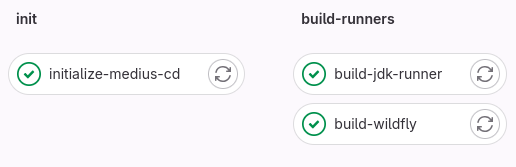
\includegraphics[width=8.5cm]{figures/java-projekt-cevovod-izvajalne-slike.png}
    \end{center}
\caption{Cevovod za gradnjo izvajalnih slik.}
\label{fig:java-projekt-gradnja-izvajalnih-slik}
\end{figure}

Nato lahko zaženemo cevovod aplikacije, ki je prikazan na sliki \ref{fig:java-cevovod} in vsebuje naslednje naloge:
\begin{itemize}
    \item Priprava komponente Medius CD
    \item Gradnja aplikacije - aplikacija se zgradi z orodjem Maven, ki po gradnji zažene tudi teste enot.
    \item Gradnja vsebniških slik - naloga zažene podrejen cevovod, ki vsebuje nalogo za gradnjo aplikacijske slike.
    \item Preverjanje kakovosti - naloga, ki z orodjem Maven zažene vtičnik za preverjanje kakovosti platforme SonarQube.
    \item Objava vsebniških slik
    \item Namestitev aplikacije - naloga zažene podrejen cevovod, ki vsebuje naloge za namestitev aplikacije v različna okolja na gruči Kubernetes.
    \item Naloge za izdajo nove verzije
\end{itemize}

\begin{figure}
    \begin{center}
        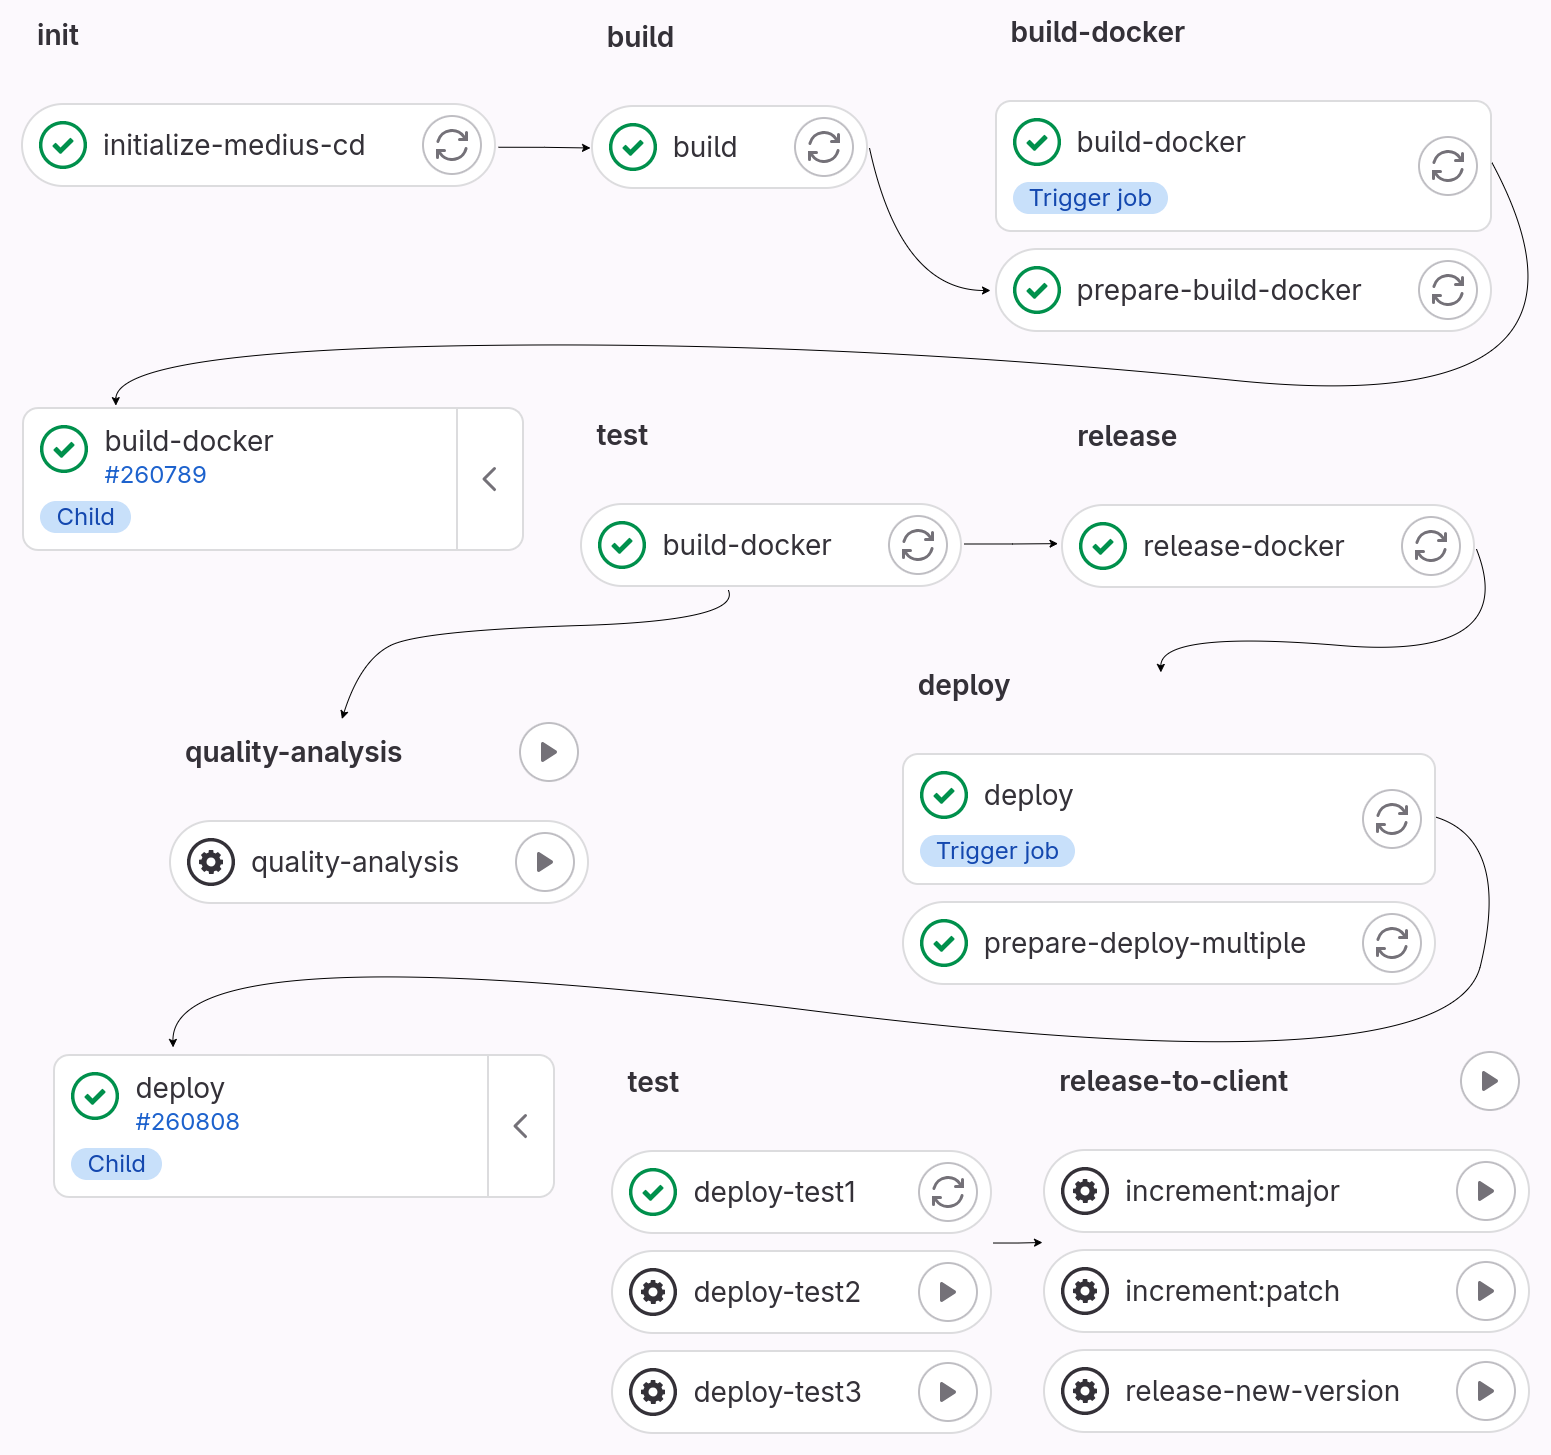
\includegraphics[width=13.5cm]{figures/java-cevovod.png}
    \end{center}
\caption{Cevovod projekta v programskem jeziku Java.}
\label{fig:java-cevovod}
\end{figure}

\section{Projekt v programskem jeziku TypeScript}
\label{sec:typescript-projekt}
V tem poglavju bomo predstavili postavitev cevovoda projekta, ki vsebuje programje napisano v programskem jeziku TypeScript in za gradnjo uporablja orodje pnpm. Projekt vsebuje interno razvito knjižnico za razvoj čelnih aplikacij z ogrodjem Angular in čelno aplikacijo, ki se uporablja za demonstracijo uporabe knjižnice. Čelna aplikacija se povezuje na zaleTole je typscriptdni sistem, ki je del drugega projekta.

\subsection{Konfiguracija cevovoda}
Podobno kot pri prejšnjem projektu, smo na konfiguracijski strežnik Consul dodali datoteko \texttt{config\_file} z naslednjo vsebino:
\begin{verbatim}
# Globalne spremenljivke
variables:
  KUBECONFIG_CONSUL_PATH: "default/.kube/config.v24"
  EXPOSED_SUFFIX: "apps.kubetest5.int.medius.si"
# Servisi
services:
- dir: "./apps/sampler"
  environments:
  - name: "sbm1"
    variables:
      AUTO_DEPLOY: "true"
      coreBasePath: "https://qs-sbm1-qs.apps.medius.si"
# Integracijski testi
it:
  deployments:
    - project: "medius/angular-common/medius-angular"
      branch: "dev"
    - project: "medius/angular-common/quarkus-sampler"
      branch: "dev"
\end{verbatim}

Ponovno smo nastavili globalni spremenljivki \texttt{KUBECONFIG\_CONSUL\_PATH} in \texttt{EXPOSED\_SUFFIX} ter dodali servis, ki predstavlja čelno aplikacijo. Servisu smo s ključno besedo \texttt{dir} nastavili imenik v repozitoriju, v katerem se nahaja in dodali spremenljivko \texttt{coreBasePath}, ki jo potrebuje za namestitev. Nato smo pod ključno besedo \texttt{it} definirali še namestitvi, ki jih cevovod potrebuje za izvajanje integracijskih testov. Prva namestitev je čelna aplikacija, druga namestitev pa zaledna aplikacija, s katero čelna aplikacija komunicira.

\subsection{Izvajalne slike}
V imenik \texttt{runner-images} smo dodali datoteko Docker, ki definira izvajalno sliko imenovano \texttt{node-pnpm} za izvajanje nalog v cevovodu. Za osnovo uporablja sliko \texttt{rocky-with-tools}, nato sledijo ukazi za namestitev dodatnih orodji, ki jih potrebujemo za izvajanje nalog, med drugimi tudi Node in pnpm.

\subsection{Aplikacijska vsebniška slika}
Datoteka, ki definira aplikacijsko vsebniško sliko za osnovo uporablja sliko \texttt{nginx}. Ostali ukazi skopirajo vse potrebne datoteke za zagon aplikacije in nastavijo skript, ki se ob zagonu vsebnika zažene.

\subsection{Konfiguracijske datoteke platforme Kubernetes}
Konfiguracijske datoteke za namestitev aplikacije na gručo platforme Kubernetes so zelo podobne tistim v prejšnjem projektu. Razlika je zgolj v tem, da se tu vse nahajajo v imeniku \texttt{k8s}, saj aplikacijo vedno nameščamo na gručo iste verzije.

\subsection{Konfiguracijske datoteke cevovoda}
Tudi tu za definicijo cevovoda dodamo enake datoteke kot prej. V datoteki \texttt{.gitlab/.build-runners.yml} uporabimo predlogo za gradnje izvajalne slike \texttt{node-pnpm}:
\begin{verbatim}
include:
  - project: 'medius/ci-tools/medius-cd'
    ref: v4.5.1
    file:
      - '/gitlab-ci/templates/runners/jobs/.node-pnpm.yaml' 
\end{verbatim}
V datoteki \texttt{.gitlab/.main.yml} pa uporabimo predlogo za cevovod projekta, ki uporablja okolje Node in orodje pnpm, ter nastavimo nekaj spremenljivk na vrednost \texttt{true}, kar v cevovod doda nekaj dodatnih nalog:
\begin{itemize}
    \item \texttt{RELEASE\_PACKAGE} - objava paketa na centralni repozitorij Nexus.
    \item \texttt{RELEASE\_PACKAGE\_PUBLIC} - objava paketa na javni register npm.
    \item \texttt{IT\_RUN} - zagon integracijskih testov.
    \item \texttt{IT\_DEPLOY} - namestitev aplikacij v okolje za integracijske teste.
    \item \texttt{IT\_NAMESPACE\_CLEAN\_UP} - brisanje okolja integracijskih testov.
\end{itemize}
Obenem prilagodimo nalogo za gradnjo aplikacije tako, da v artefakte naloge zapakira dodatne datoteke. Celotna vsebina datoteke je videti tako:
\begin{verbatim}
include:
  - project: 'medius/ci-tools/medius-cd'
    ref: v4.5.1
    file:
      - '/gitlab-ci/templates/node/pnpm/.pnpm-all.yaml' 

variables:
  RELEASE_PACKAGE: "true"
  RELEASE_PACKAGE_PUBLIC: "true"
  IT_RUN: "true"
  IT_DEPLOY: "true"
  IT_NAMESPACE_CLEAN_UP: "true"

build:
  artifacts:
    paths:
      - "${CACHE_PATH}/apps/*/dist/"
      - "${CACHE_PATH}/libs/*/dist/"
      - pnpm-lock.yaml
\end{verbatim}

\subsection{Delovanje cevovoda}
Potem, ko smo zgradili izvajalne slike s cevovodom za gradnjo izvajalnih slik, lahko zaženemo cevovod aplikacije, ki ga lahko vidimo na sliki \ref{fig:typescript-cevovod} in vsebuje naslednje naloge:
\begin{itemize}
    \item Priprava spremenljivk za integracijske teste - naloga iz konfiguracijskega strežnika Consul prenese datoteko s spremenljivkami, ki jih cevovod potrebuje za izvajanje integracijskih testov. V tem primeru vsebuje zaledna naslova zaledne in čelne aplikacije, ki bosta nameščena v okolju za integracijske teste.
    \item Priprava komponente Medius CD
    \item Gradnja aplikacije
    \item Statična analiza kode (ang. lint)
    \item Testi enot
    \item Gradnja vsebniških slik - naloga zažene podrejen cevovod, ki vsebuje nalogo za gradnjo aplikacijske slike.
    \item Namestitev aplikacij v okolje za integracijsko testiranje - naloga zažene podrejen cevovod, ki zažene nalogo za namestitev čelne aplikacije in zažene podrejen cevovod za namestitev zaledne aplikacije, ki jo čelna aplikacija uporablja v projektu, ki vsebuje zaledno aplikacijo. Cevovod je prikazan na sliki \ref{fig:typescript-projekt-it-cevovod}
    \item Zagon integracijskih testov
    \item Preverjanje kakovosti kode
    \item Izdaja vsebniških slik
    \item Naloge za izdajo paketa na centralni repozitorij Nexus in javni register npm
    \item Namestitev aplikacij - naloga zažene podrejen cevovod, ki vsebuje naloge za namestitev aplikacije v različna okolja na gruči Kubernetes.
    \item Brisanje okolja integracijskih testov
    \item Naloge za izdajo novih verzij
\end{itemize}

\begin{figure}
    \begin{center}
        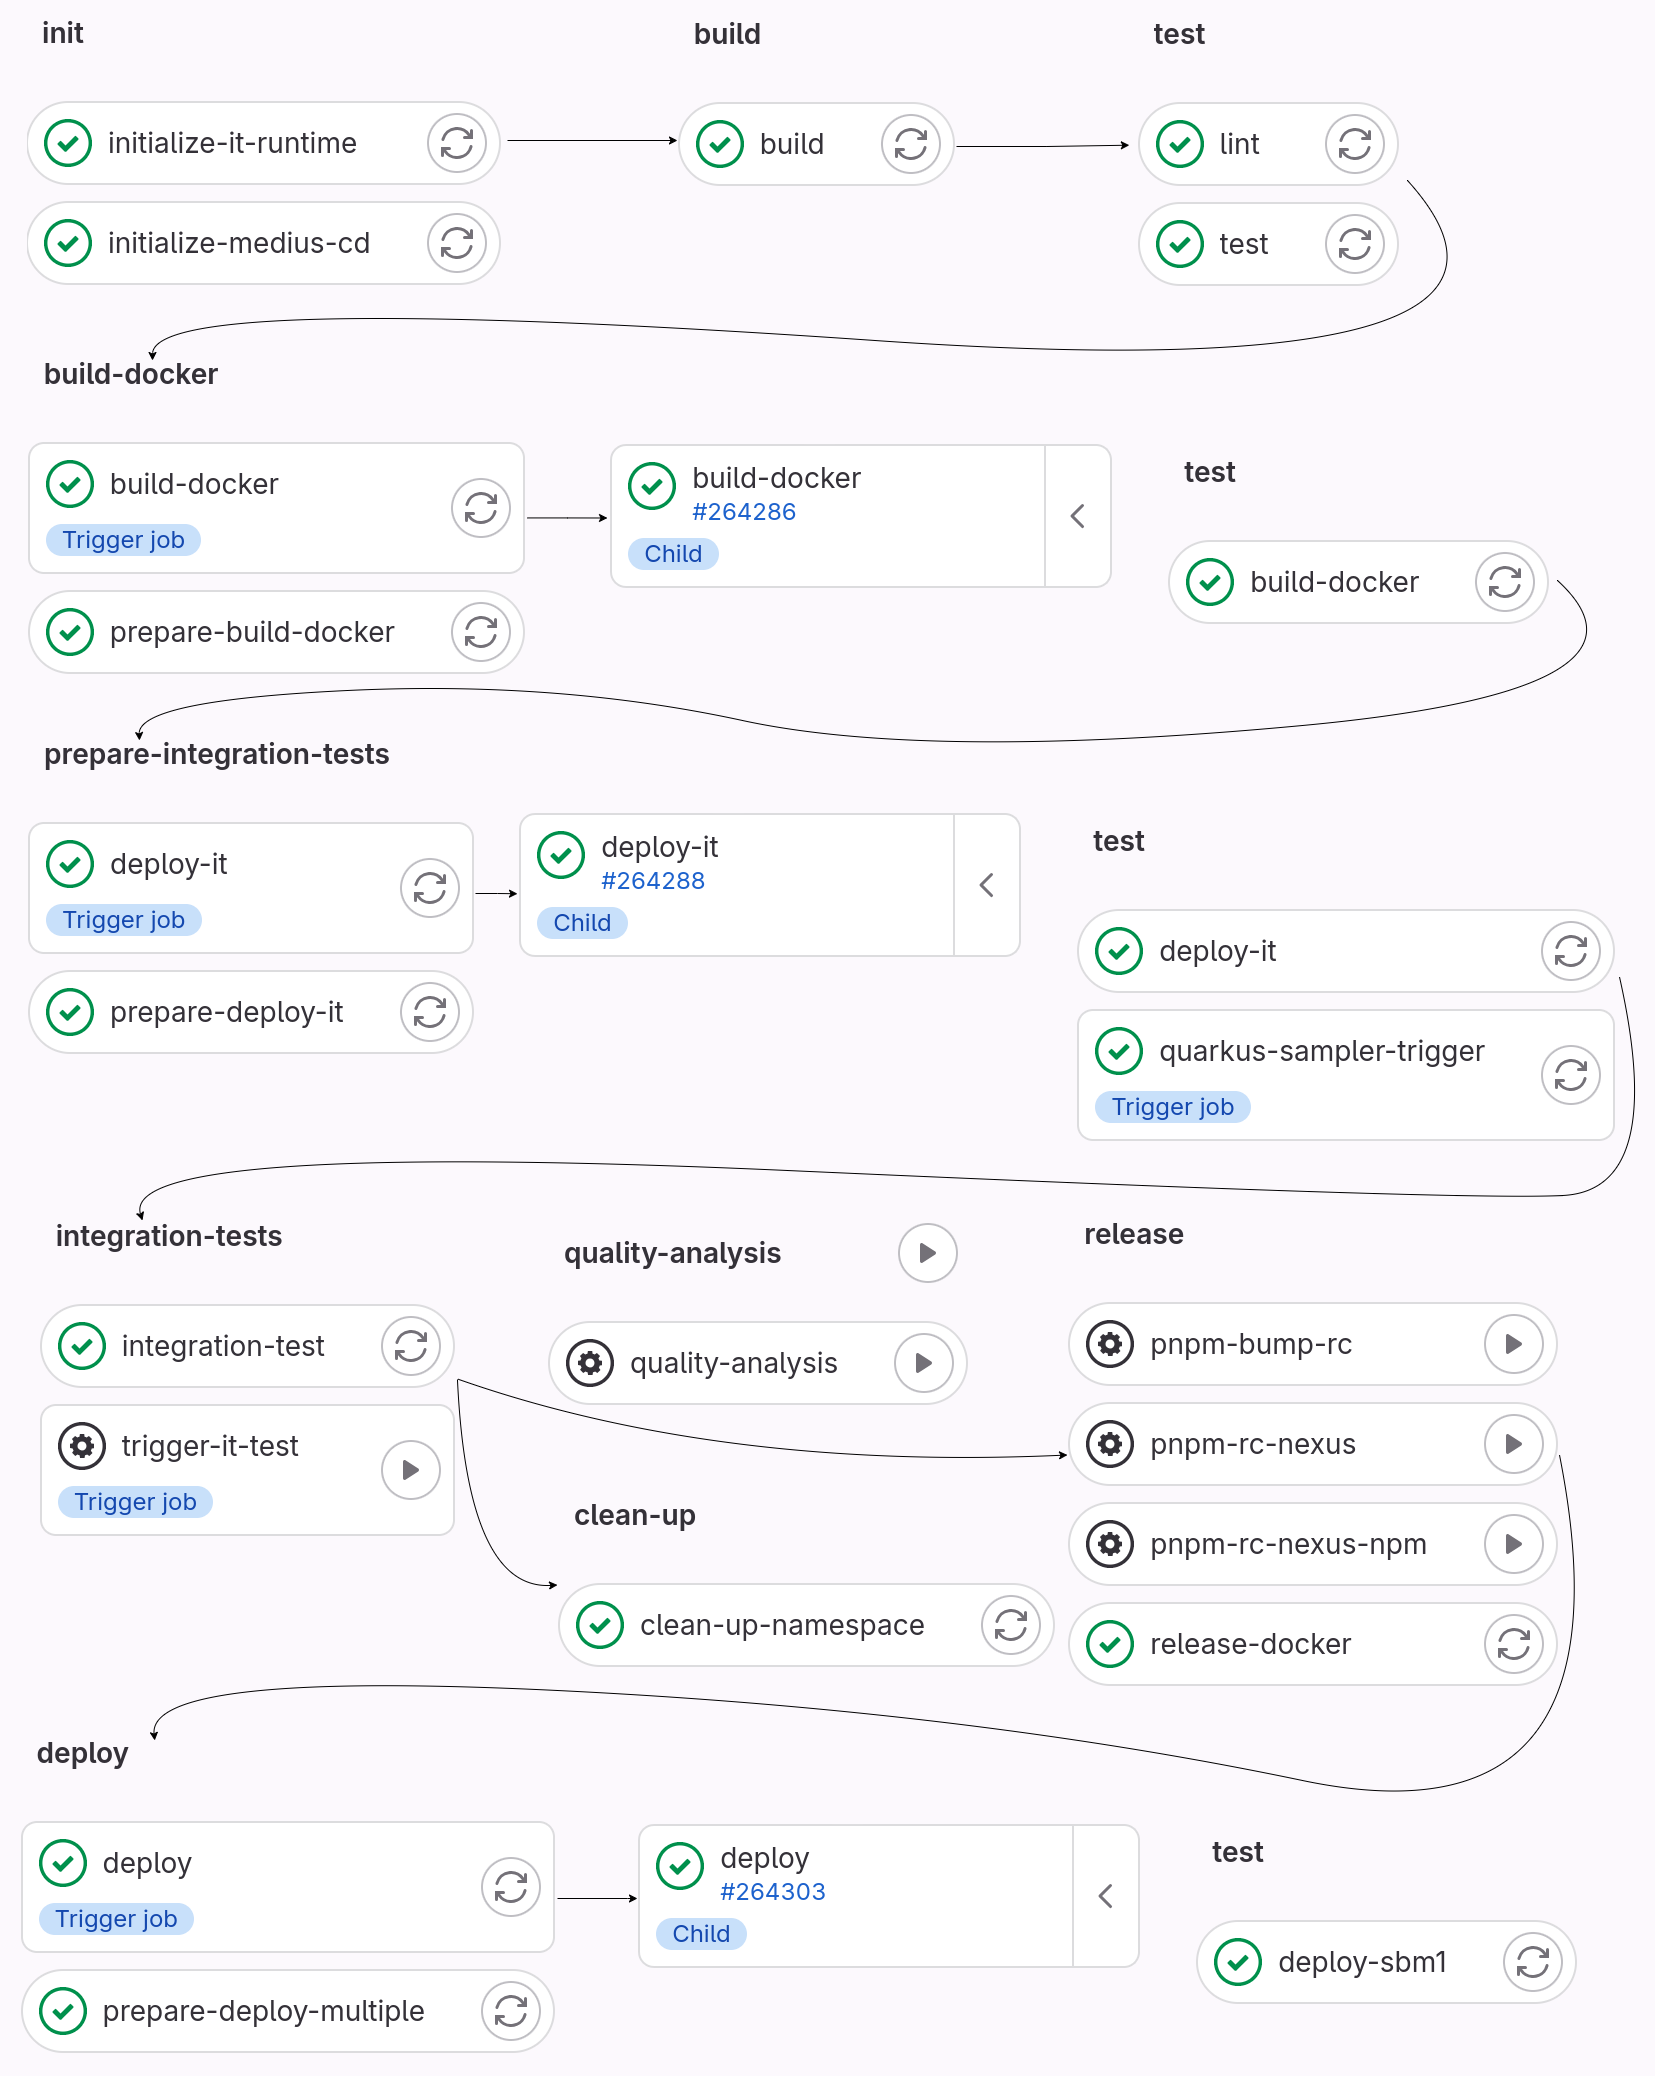
\includegraphics[width=13.5cm]{figures/typescript-cevovod.png}
    \end{center}
\caption{Cevovod projekta v programskem jeziku TypeScript.}
\label{fig:typescript-cevovod}
\end{figure}

\section{Projekt v programskem jeziku Python}
\label{sec:python-projekt}
V tem poglavju bomo predstavili postavitev cevovoda projekta, ki vsebuje dve aplikaciji napisani v programskem jeziku Python. Aplikaciji uporabljata knjižnico FastAPI, s katero izpostavljata končne točke za prepoznavanje in redakcijo občutljivih podatkov v besedilu s pomočjo modelov strojnega učenja.

% Naročnik ne uporablja platforme GitLab, zato se cevovod izvaja samo v podjetju. TODO

\subsection{Konfiguracija cevovoda}
Zaradi večje občutljivosti projekta, smo pri temu projektu datoteko \texttt{config\_file} raje shranili v spremenljivko GitLab. Datoteka ima naslednjo vsebino:
\begin{verbatim}
variables:
    EXPOSED_SUFFIX: "apps.kubetest-ai.int.medius.si"
    CREATE_NAMESPACE: "false"
    AUTO_DEPLOY: "true"
services:
  - name: anonymizer
    variables:
      DOCKERFILE_PATH: "Dockerfile.stagebuild-anonymizer"
      APP_PORT: 8001
      GPU_CORE: 0
    environments:
      - name: "prod"
        variables:
          KUBECONFIG: "TEST_KUBECONFIG"
          AUTO_DEPLOY: "false"
      - name: "dev"
        variables:
          KUBECONFIG: "DEV_KUBECONFIG"
      - name: "stg"
        variables:
          KUBECONFIG: "STG_KUBECONFIG"
  - name: analyzer
    variables:
      DOCKERFILE_PATH: "Dockerfile.stagebuild"
      APP_PORT: 8000
      GPU_CORE: 0
      BUILD_ARGS: "NER_VERSION=1.2.3,SLONER_VERSION=1.2.3"
    environments:
      - name: "prod"
        variables:
          KUBECONFIG: "TEST_KUBECONFIG"
          AUTO_DEPLOY: "false"
      - name: "dev"
        variables:
          KUBECONFIG: "DEV_KUBECONFIG"
      - name: "stg"
        variables:
          KUBECONFIG: "STG_KUBECONFIG"
          GPU_CORE: 1
\end{verbatim}
Zopet smo nastavili globalno spremenljivko \texttt{EXPOSED\_SUFFIX} in dodali dve dodatni globalni spremenljivki: 
\begin{itemize}
    \item \texttt{CREATE\_NAMESPACE} z vrednostjo \texttt{false}, ki izklopi ustvarjanje imenskega prostora na gruči Kubernetes, če ta še ne obstaja. To smo naredili zato, ker je na gruči že pripravljen imenski prostor.
    \item \texttt{AUTO\_DEPLOY} z vrednostjo na \texttt{true}, ki povzroči, da se vse naloge za namestitev aplikacij na glavni veji avtomatsko zaženejo.
\end{itemize}
Ker projekt vsebuje dve aplikaciji, smo pod ključno besedo \texttt{services} definirali dva servisa: \texttt{anonymizer} in \texttt{analyzer}. Obema smo s spremenljivko \texttt{DOCKERFILE\_PATH} spremenili privzeto pot do aplikacijske datoteke Docker in nastavili še nekaj spremenljivk, ki jih potrebujeta za namestitev. Pri servisu \texttt{analyzer} smo dodali tudi spremenljivko \texttt{BUILD\_ARGS}, ki vsebuje argumente v formatu \texttt{ime\_spremenljivke=vrednost}, ločene z vejico, ki se uporabijo ob gradnji slike. Oba servisa imata tri okolja: \texttt{prod}, \texttt{dev} in \texttt{stg}. Vsako okolje uporablja drugo gručo Kubernetes, zato ima vsako okolje s spremenljivko \texttt{KUBECONFIG} nastavljeno svojo konfiguracijsko datoteko za povezavo in avtentikacijo na gručo Kubernetes. Za okolje \texttt{prod} smo prepisali globalno spremenljivko \texttt{AUTO\_DEPLOY} z vrednostjo \texttt{false}, saj ne želimo, da se naloga za namestitev na produkcijsko okolje avtomatsko zažene.

\subsection{Izvajalne slike}
V imenik \texttt{runner-images} smo dodali datoteko, ki definira izvajalno vsebniško sliko \texttt{python} za izvajanje nalog v cevovodu. Za osnovo uporablja \texttt{rocky-wi\-th-tools}, nato sledijo ukazi za namestitev prevajalnika za programski jezik Python in knjižnic wheel, twine in tox.

\subsection{Aplikacijski vsebniški sliki}
Servisa uporabljata vsak svojo vsebniško sliko, ki se nahajata v korenskem imeniku projekta. V konfiguracijski datoteki cevovoda \texttt{config\_file} smo zato spremenili privzeti poti do slik. Obe datoteki sliki, ki se uporabljata za namestitev servisov, za osnovo uporabljata sliko \texttt{python:3.9-slim} in sta sestavljeni iz več delov: priprava okolja, namestitev odvisnosti in gradnja aplikacije ter zagon aplikacije. Posebnost teh dveh slik je, da ne potrebujeta vnaprej zgrajene aplikacije, vendar aplikacijo zgradita v procesu gradnje slike.

\subsection{Konfiguracijske datoteke platforme Kubernetes}
Tudi tu so konfiguracijske datoteke za namestitev aplikacije podobne tistim, ki smo jih uporabili v prejšnjih dveh projektih. Nahajajo se v imeniku \texttt{k8s} in se uporabljajo za oba servisa. Vse vrednosti, ki se morda razlikujejo med servisoma, so v konfiguracijske datoteke dodane kot spremenljivke, ki se pred namestitvijo na gručo Kubernetes nadomestijo s ustreznimi vrednostmi, kot smo opisali v poglavju \ref{subsec:namestitev-aplikacije}.

\subsection{Konfiguracijske datoteke cevovoda}
Za vzpostavitev cevovoda smo ponovno dodali enake datoteke kot prej, vendar smo v datoteki \texttt{.gitlab/.build-runners.yml} uporabili predlogo za gradnjo izvajalne slike \texttt{python}:
\begin{verbatim}
include:
  - project: 'medius/ci-tools/medius-cd'
    ref: v4.5.1
    file:
      - '/gitlab-ci/templates/runners/jobs/.python.yaml' 
\end{verbatim}
V datoteki \texttt{.gitlab/.main.yml} pa smo uporabili predlogo za cevovod aplikacije, ki uporablja programski jezik Python. Ker naloga za gradnjo vsebniških slik ne potrebuje zgrajene aplikacije, smo nastavili vrednost spremenljivke \texttt{DOCKER\_NEEDS\_BUILD} na \texttt{false} in s pravili odstranili nalogo za gradnjo aplikacije. Odstranili pa smo tudi nalogo za izvajanje testov enot, ker projekt trenutno še nima testov enot.
\begin{verbatim}
include:
  - project: 'medius/ci-tools/medius-cd'
    ref: v4.5.1
    file:
      - '/gitlab-ci/templates/python/.python-all.yaml'

variables:
  DOCKER_NEEDS_BUILD: "false"

build:
  rules:
    - when: never

test:
  rules:
    - when: never
\end{verbatim}

\subsection{Delovanje cevovoda}
Po zgrajenih izvajalnih vsebniških slikah lahko zaženemo cevovod aplikacije, ki je prikazan na sliki \ref{fig:python-projekt-cevovod} in vsebuje naslednje naloge:
\begin{itemize}
    \item Priprava komponente Medius CD
    \item Gradnja vsebniški slik - naloga zažene podrejen cevovod, ki ga lahko vidimo na sliki \ref{fig:python-projekt-cevovod} in vsebuje nalogi za gradnjo obeh aplikacijskih slik.
    \item Izdaja vsebniških slik
    \item Namestitev aplikacij - naloga zažene podrejen cevovod, ki ga lahko vidimo na sliki \ref{fig:python-projekt-cevovod} in vsebuje naloge za namestitev aplikacij v različna okolja.
    \item Naloge za izdajo novih verzij
\end{itemize}

\begin{figure}
    \begin{center}
        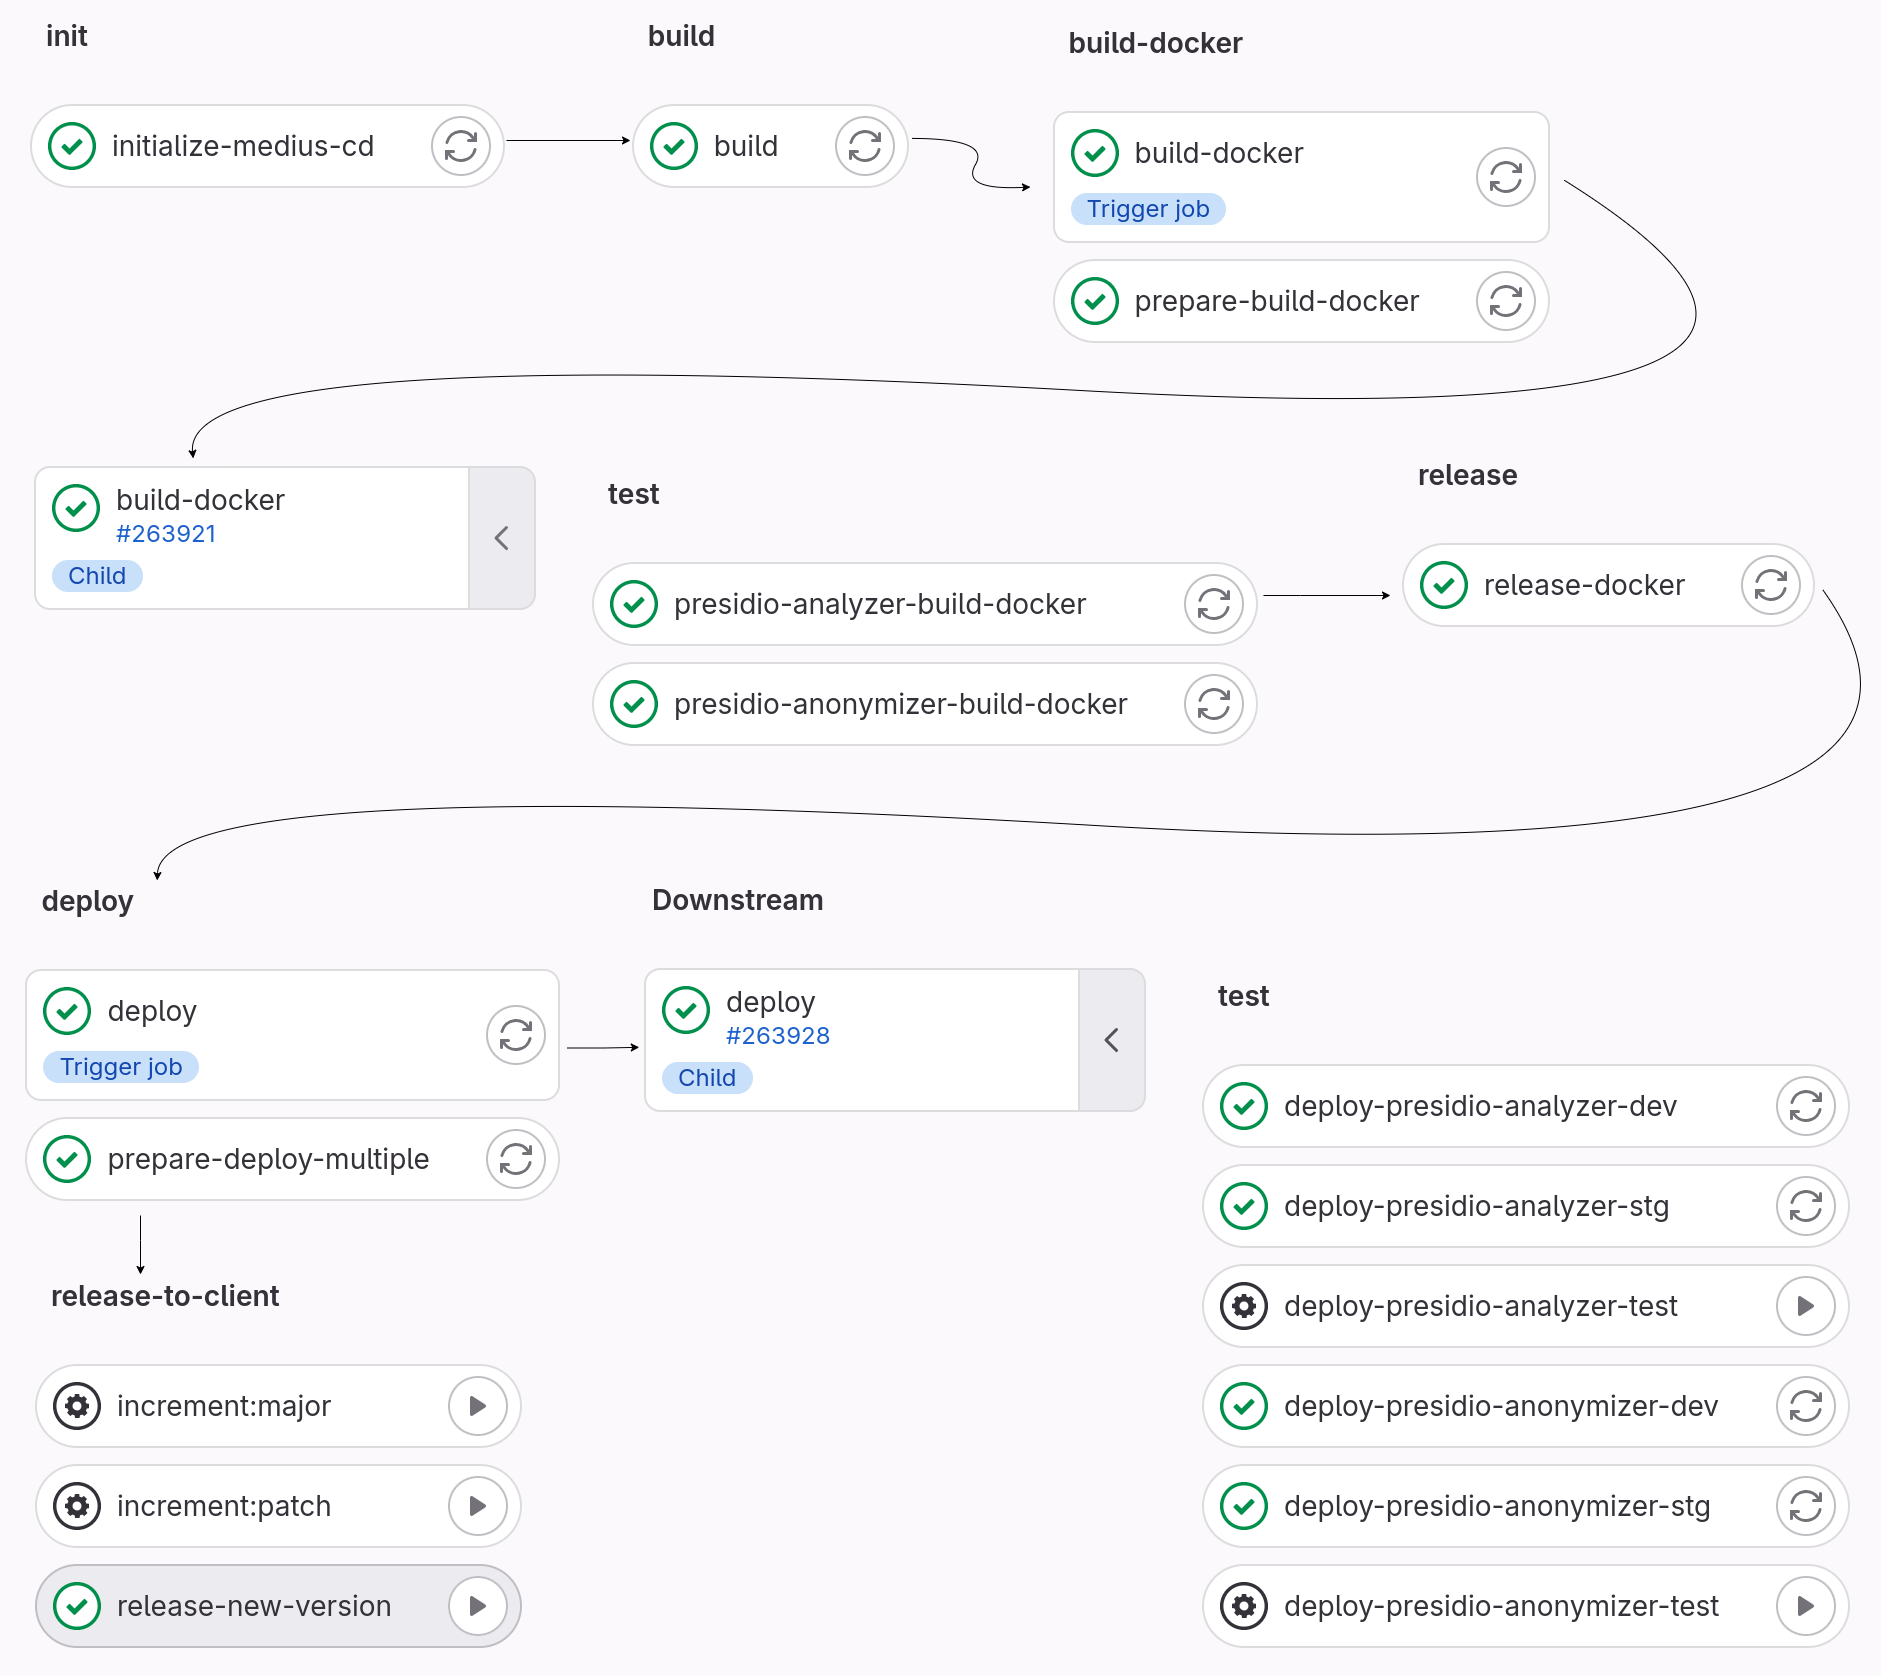
\includegraphics[width=13.5cm]{figures/python-cevovod.png}
    \end{center}
\caption{Cevovod projekta.}
\label{fig:python-projekt-cevovod}
\end{figure}


\section{Vtičnik GitLab Template Lint}
\label{sec:rezultati-vtičnik-gitlab-template-lint}
Vtičnik GitLab Template Lint znatno olajša in pospeši razvoj kompleksnejših cevovodov z orodjem Gitlab CI/CD. Pred razvojem vtičnika smo konfiguracijske datoteke orodja GitLab CI/CD preverjali tako, da smo vsebino datotek kopirali v orodje platforme GitLab ali pa spremembe kar odrinili v repozitorij in spremljali status cevovoda. Z vtičnikom odkrijemo napake že v integriranem okolju med pisanjem konfiguracije. Obenem vtičnik v urejevalniku kode konfiguracijskih datotek prikazuje predogled vsebine združene konfiguracijske datoteke kar olajša iskanje napak. Delovanje je prikazano na sliki \ref{fig:gitlab-template-lint-rezultati-2}.

\begin{figure}
    \begin{center}
        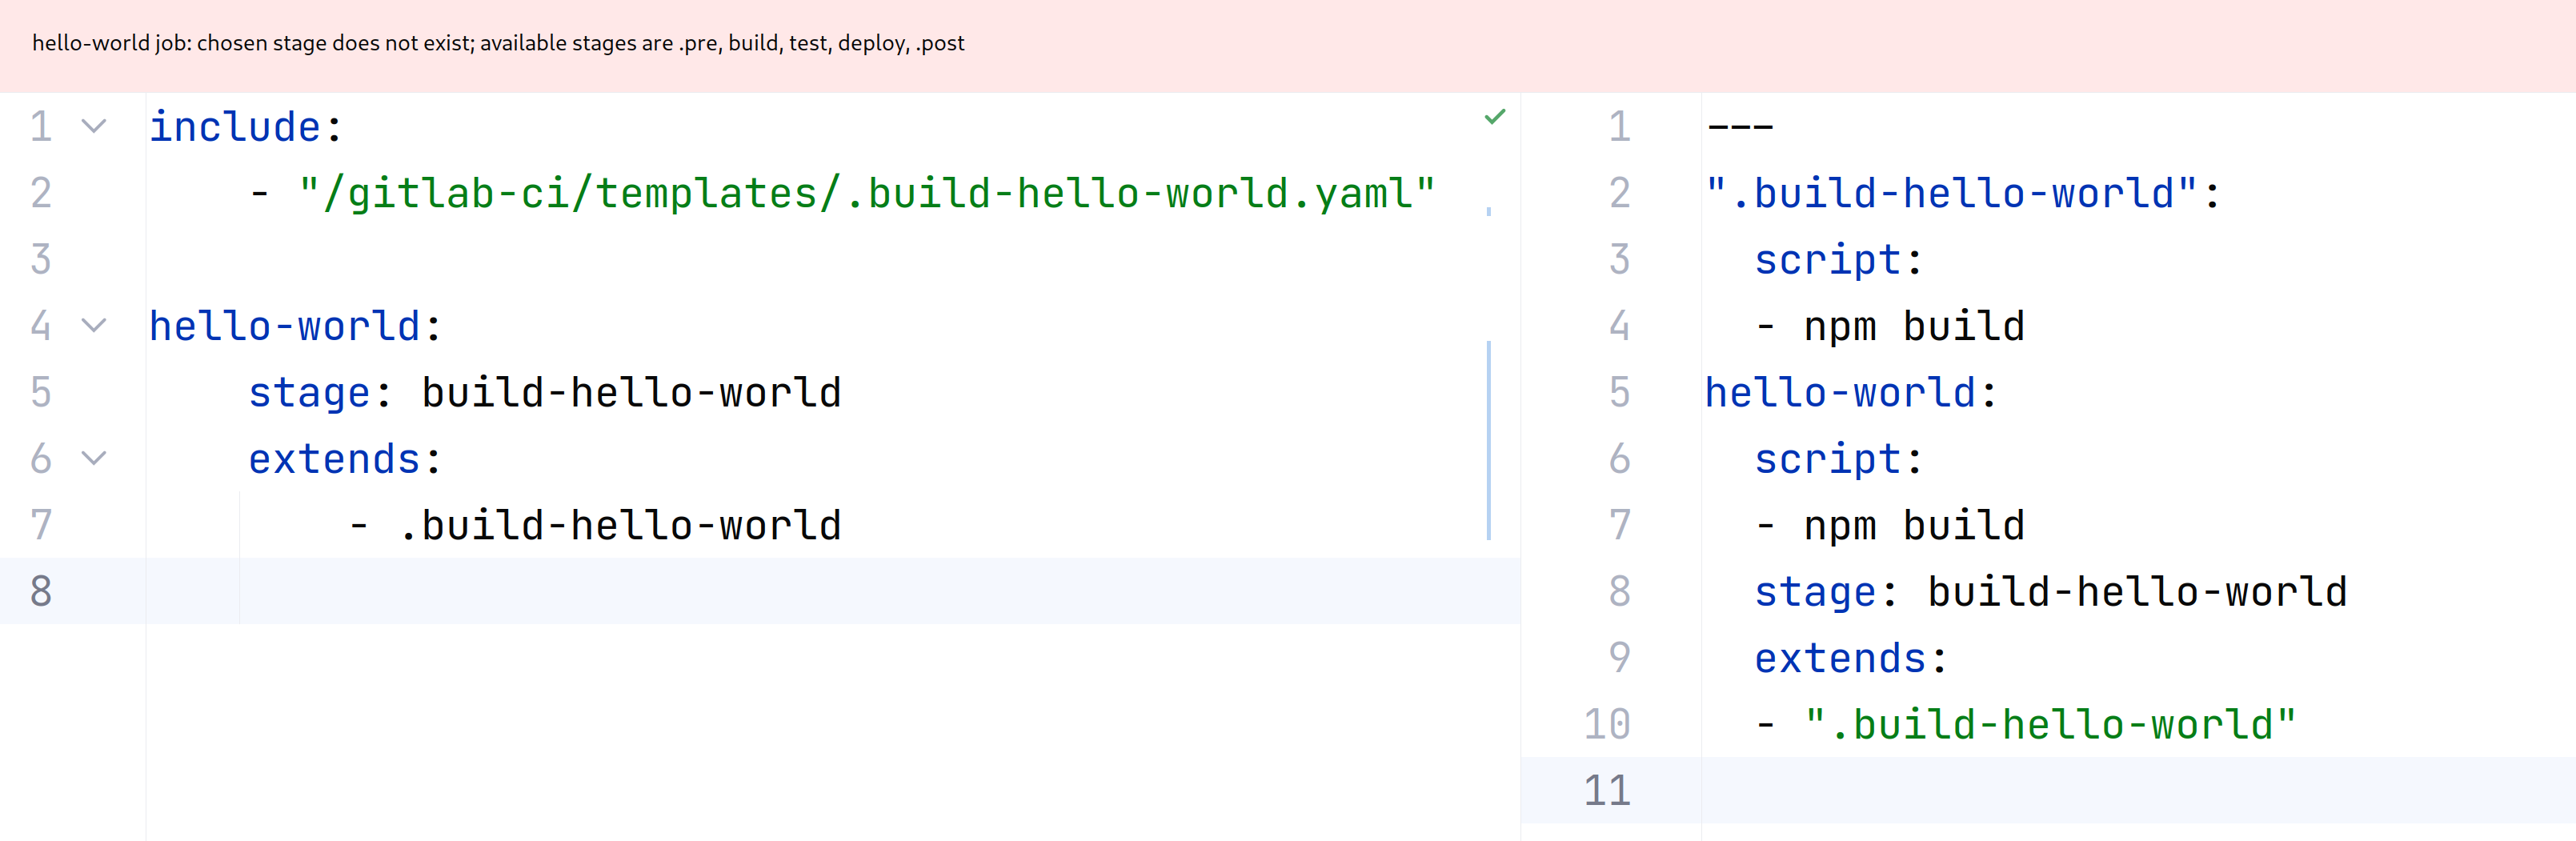
\includegraphics[width=13.5cm]{figures/gitlab-template-lint-rezultati-2.png}
    \end{center}
\caption{Delovanje vtičnika.}
\label{fig:gitlab-template-lint-rezultati-2}
\end{figure}

\subsection{Omejitev vtičnika}
\label{subsec:rezultati-vtičnik-gitlab-template-lint-omejitve}
Končni točki za preverjanje konfiguracijskih datotek GitLab CI/CD lahko v zahtevku pošljemo samo eno konfiguracijsko datoteko naenkrat. Vse datoteke, ki so v poslani datoteki dodane s ključno besedo \texttt{include} se preberejo iz repozitorija oziroma spletnega naslova, ki je nastavljen. To pomeni, da če spreminjamo več konfiguracijskih datotek hkrati, vtičnik ne deluje pravilno, saj končna točka za preverjanje uporablja starejše različice datotek. To bi lahko rešili, če bi končna točka za preverjanje konfiguracijskih datotek lahko sprejela več datotek naenkrat.

\subsection{Objava vtičnika}
Vsa koda razvitega vtičnika je javno objavljena na platformi GitHub\footnote{\url{https://github.com/Blarc/gitlab-template-lint-plugin}}, kjer se ob vsaki izdaji nove različice zažene tudi cevovod za objavo na tržnico vtičnikov podjetja JetBrains\footnote{\url{https://plugins.jetbrains.com/plugin/19411-gitlab-template-lint}}. Na ta način lahko uporabniki integriranih okolji podjetja JetBrains vtičnik enostavno namestijo v svoje okolje preko vgrajene funkcionalnosti za namestitev vtičnikov. Prva različica vtičnika je bila na tržnici vtičnikov objavljena 24. junija 2022. Do današnjega dne, 7. septembra 2023, pa smo objavili še 24 različic. Potrebo po vtičniku dokazuje tudi 39 zvezdic na platformi GitHub in 26645 namestitev vtičnika v integrirana okolja podjetja JetBrains.


%----------------------------------------------------------------
% Poglavje 6 - Zaključek
%----------------------------------------------------------------


\chapter{Zaključek}
\label{ch:zaključek}
V predstavljenem delu smo opisali poslovno kritične aplikacije in njihove lastnosti. Predstavili smo proces neprekinjene integracije in dostave ter zakaj predstavlja pomemben del pri razvoju poslovno kritičnih aplikacijah. Opisali smo tudi dva različna primera strukture projekta, ki vplivata na organizacijo razvoja, tehnologije ter orodja in ogrodja, ki smo jih uporabili za razvoj cevovoda neprekinjene integracije in dostave.

Razvili smo komponento za vzpostavitev neprekinjene integracije in dostave na platformi GitLab imenovano Medius CD. Cilj komponente je poenotenje cevovodov, zmanjšanje podvojene konfiguracije in kode ter olajšanje vzdrževanja. To smo dosegli z uporabo predlog konfiguracijskih datotek GitLab, ki definirajo naloge v cevovodu in uporabljajo skripte komponente Medius CD. Skripti napisani v jeziku Bash so parametrizirani in jih lahko zaganjamo s poljubnimi parametri. Te lahko nastavimo v konfiguracijski datoteki. S takim pristopom olajšamo vzdrževanje spremenljivk in dosežemo visoko nivojsko abstrakcijo neprekinjene integracije in dostave tako v razvojnem okolju ter okolju naročnika. Na ta način lahko v cevovodu:
\begin{itemize}
    \item zgradimo aplikacijo
    \item zaženemo teste enot
    \item zgradimo več različnih aplikacijskih vsebniških slik
    \item zaženemo integracijske teste
    \item namestimo aplikacijo v različna okolja
    \item izdamo novo različico projekta
\end{itemize}

Razvite konfiguracijske datoteke orodja GitLab CI/CD s podporo skript komponente Medius CD podpirajo izvajanje cevovodov CI/CD za projekte napisane v treh različnih programskih jezikih - Java, TypeScript in Python.

Na podlagi analize predlagamo novo umestitev procesa gradnje in shranjevanja izvajalnih slik. S predlaganim pristopom rešimo vodenje različic izvajalnih slik in s tem bistveno olajšamo vzdrževanje projekta.

Uporabo komponente smo predstavili na cevovodih treh projektov, ki vsebujejo aplikacije razvite v različnih programskih jezikih. Opisali smo kako lahko cevovod uporabljamo v okolju, ki zaradi varnosti nima dostopa do interneta, kako vzpostavimo cevovod v projektu, ki vsebuje programsko knjižnico in aplikacijo hkrati ter kako lahko v cevovodu enega projekta zgradimo in namestimo več aplikacij naenkrat. Pokazali smo kako lahko cevovod takšnim različnim zahtevam enostavno prilagodimo s konfiguracijsko datoteko brez večjih posegov v kodo.

Razvita komponenta je zelo stabilna in pripravljena za uporabo, vendar ima še veliko prostora za izboljšave. Skript, ki ga uporabljamo za ustvarjanje konfiguracijskih datotek za namestitev na gručo Kubernetes omenjen v poglavju \ref{subsec:namestitev-aplikacije}, bi lahko nadomestili z orodjem kustomize\footnote{\url{https://kustomize.io/}}. Trenutno so cevovodi pripravljeni za gradnjo vsebnikov z orodjema kaniko in Docker, lahko pa bi podprli tudi druga orodja, kot so: Podman, Buildah, BuildKit, containerd idr. Pomemben manjkajoči del pa predstavlja tudi vodenje različic zagonskih slik. Trenutno zagonske slike redno posodabljamo brez da spremenimo številko različice zagonske slike. To lahko privede do težav, če želimo zagnati cevovod aplikacije, ki je starejše različice.

Predstavljeno magistrsko delo povzema metodologijo za vzpostavitev CI/CD in s tem izpostavlja izzive, napake in izboljšave na primeru resničnih projektov poslovno kritičnih aplikacij. Opiše obstoječa orodja, ki so del napredne uporabe neprekinjene integracije in dostave v visoko tehnoloških razvojnih podjetjih. Izpostavi kompromise in jih v praksi udejanji v predstavljeni komponenti za razvoj cevovodov neprekinjene integracije in dostave - Medius CD. Kot dodatno orodje za razvoj cevovodov z orodjem GitLab CI/CD avtor razvije tudi vtičnik Gitlab Template Lint za uporabo v integriranem okolju IntelliJ IDEA. Vtičnik uporablja širša interesna skupina razvijalcev DevOps po vsem svetu.

% Razvite konfiguracijske datoteke GitLab in skripti v programskem jeziku Bash se uporabljajo za vzpostavitev cevovodov na projektih poslovno kritičnih aplikacij iz resničnega sveta. Predstavljeno delo lahko zato nudi dobro izhodišče za razvoj cevovodov za neprekinjeno integracijo in dostavo in služi kot opozorilo, na kaj moramo biti pri razvijanju in vzpostavljanju takšnih cevovodov pozorni. 






% ---------------------------------------------------------------
% Appendix
% ---------------------------------------------------------------
\appendix


%----------------------------------------------------------------
% SLO: bibliografija
% ENG: bibliography
%----------------------------------------------------------------
\bibliographystyle{elsarticle-num}

%----------------------------------------------------------------
% SLO: odkomentiraj za uporabo zunanje datoteke .bib (ne pozabi je potem prevesti!)
% ENG: uncomment to use .bib file (don't forget to compile it!)
%----------------------------------------------------------------
\bibliography{bibliography}


\end{document}
